\chapter{Analysis Strategy}
\label{ch:analysis}

This chapter will present the strategies used to isolate ATLAS data events most consistent with the SVJ model and to estimate the relevant background. The data and MC samples discussed in Chapter~\ref{ch:mc_data} are studied to create the analysis strategy, and the ML scores discussed in Chapter~\ref{ch:ml_tools} are used to isolate the most signal like events. The background is estimated from the \textit{transverse mass} (\mt) spectrum, which captures the main components of the $Z'$ decay. A \textit{preselection} selects events consistent with the SVJ topology based on basic features of the jets and \met. Preselected events are then split into a \textit{control region} (CR), \textit{validation region} (VR), and \textit{signal region} (SR). The CR and VR are used to validate the background estimation procedure. The SR is blinded during the development of the analysis strategy, and only unblinded to make the final measurements presented in Chapter~\ref{ch:results}. The final result is a polynomial fit of the \textit{transverse mass} (\mt) spectrum in the SR. The preselection, region definitions, and polynomial fit will be discussed in detail in the following sections.

\section{Transverse Mass}
\label{sec:mt}
The transverse mass \mt~is chosen as the search variable due to the potential for the SVJ signal to create a resonant shape around the mass of the $Z'$. \mt~is the total transverse mass of the two leading jets and the \met, expressed in Equation~\ref{eq:mt} as:

\begin{equation}
m_T^2 = [E_{T,jj} + \met~]^2 - [\vec{p}_{T,jj} + \vec{p}_T^{\text{miss}}]^2
\label{eq:mt}
\end{equation}

where $E_{T,jj}$ is the transverse energy of the dijet system. We take $E_{T,jj} = m_{jj}^2 + |\vec{p}_{T,jj}|^2$, where $m_{jj}^2$ is the invariant mass of the two leading jets, and $\vec{p}_{T,jj}$ is the vector sum of the \pt~of the two leading jets. \mt~is selected as the search variable in place of simpler invariant mass $m_{jj}$ because substantial energy from the Z' decay is captured in the \met~. Therefore incorporating \met~into \mt~improves the resonance around the mass of the $Z'$. \par

Figure~\ref{fig:mt_mass} illustrates the resonance in \mt~of the SVJ signals. The smoothly falling background is shown in comparison to the resonant shape of the signals, which form a peak just below the associated $Z'$ mass. The lower \rinv~signals form a more distinctive resonance in \mt, while the high \rinv~signals have a much wider \mt~shape.
\begin{figure}[!htbp]
\centering
    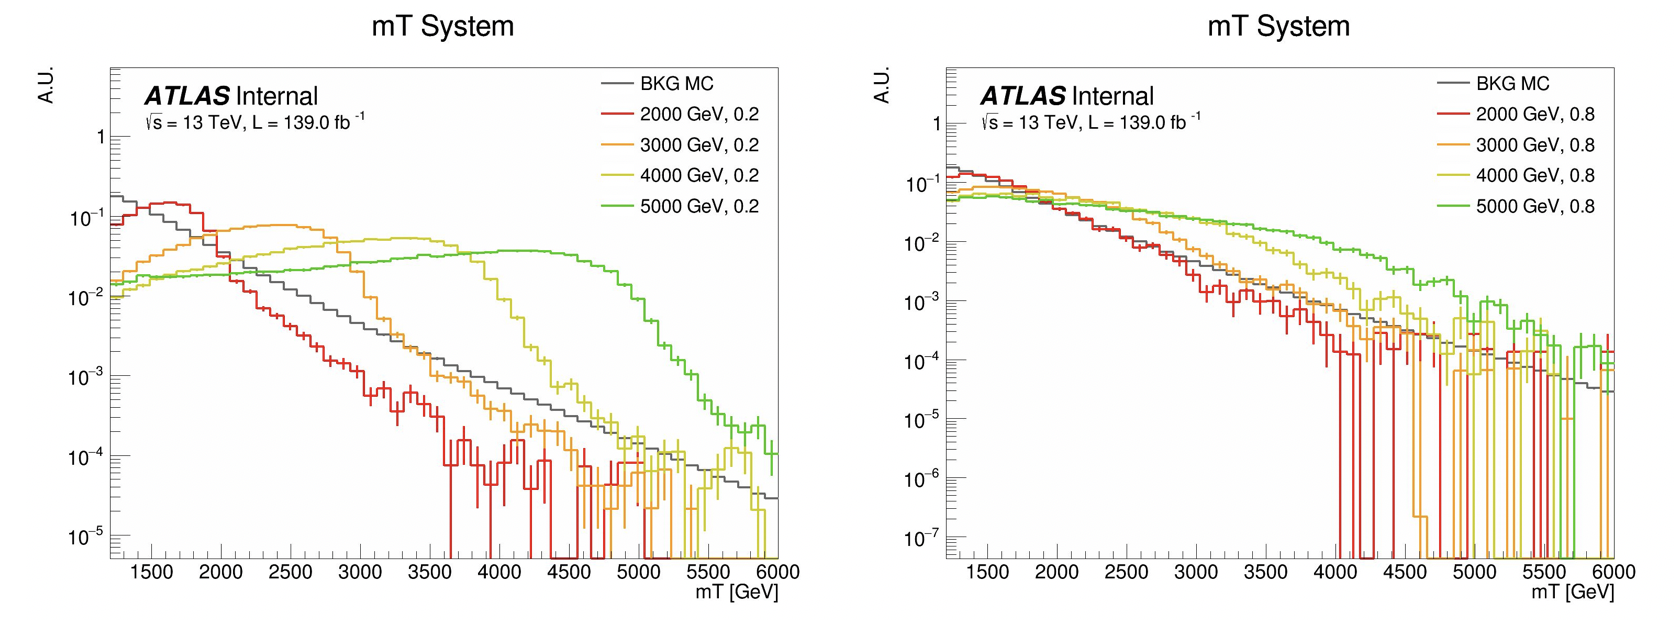
\includegraphics[width=0.98\textwidth]{figures/ch8/mt_mass_norm}
    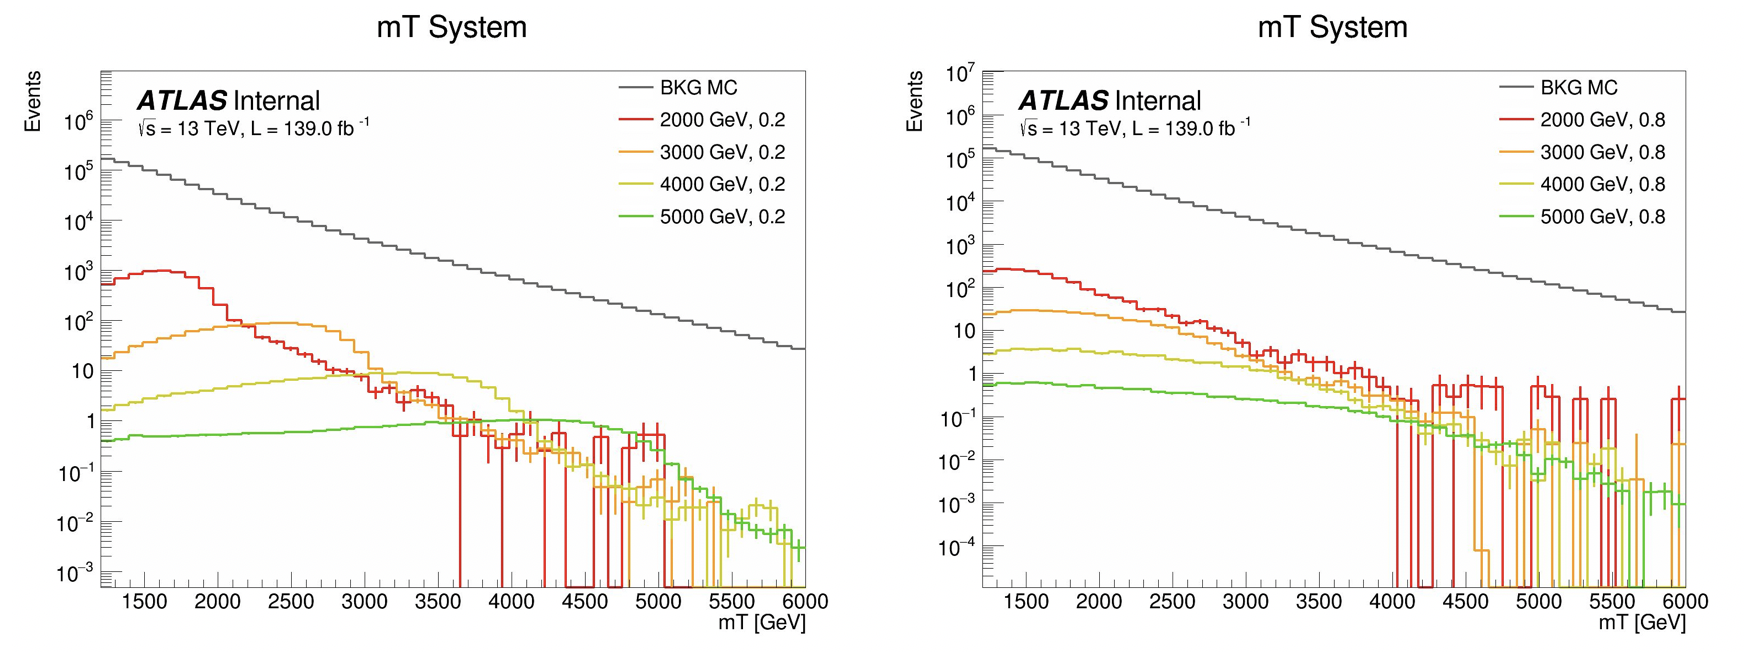
\includegraphics[width=0.98\textwidth]{figures/ch8/mt_mass_unnorm}
    \caption{The resonant shape of the SVJ signals (color) in \mt, in contrast to the smoothly falling \mt~background (grey). The top row illustrates unit normal shapes, so that the shape of the signals is more easily seen. The bottom row illustrates the signal and background scaled to their expected yield at preselection, illustrating the relative expected statistics. The \rinv~= 0.8 signals (right) boast a wider shape, making them more difficult to detect, while the \rinv~= 0.2 signals (left) produce a more narrow resonance in \mt~. The signal models are identified in the legend as ``$m_{Z'}$, \rinv''. 
    \label{fig:mt_mass}}
\end{figure}

%------------------------------------------------- 
\section{Preselection}
\label{sec:eventsel}

The preselection isolates the phase space of events that most closely match the SVJ signal topology. Each cut was determined to reduce the background and enhance signal sensitivity.
The list of preselection cuts and the motivation behind each cut are as follows. 
Here ``jets" refer to anti-$k_t$ R=0.4 jets, as discussed in Chapter~\ref{ch:part_reco}.

\begin{itemize}
\item At least 2 jets; in order to reconstruct the resonance mass
\item Leading jet ($j_1$) \pt $>$ 450 GeV; to ensure the trigger is fully efficient
\item Subleading jet ($j_2$) \pt $>$ 150 GeV; to mitigate the presence of non-collision background (Appendix~\ref{app:ncb})
\item $|\eta_{j1,j2}|$ $<$ 2.1; to ensure jets are fully within the tracker
\item $\Delta$Y$<$ 2.8 (difference in rapidity between $j_1$ and $j_2$); to ensure central production associated with the hard scatter  
\item \met $>$ 200 GeV; to restrict the phase space to events with possible dark particles 
\item \mt $>$ 1.2 TeV, to ensure a smoothly falling \mt~distribution for fitting (Section~\ref{sec:background})
\item At least 3 tracks for each of the two leading jets $j_1$ and $j_2$; to have adequate tracking information for the ML tools
\item $\Delta\Phi$($j_1$,$j_2$) $>$ 0.8; to mitigate the presence of non-collision background (Appendix~\ref{app:ncb}).
\end{itemize}

Table~\ref{fig:presel_cutflow} shows the impact of these cuts in sequence for data and signal.
\begin{table}[!htbp]
\centering
   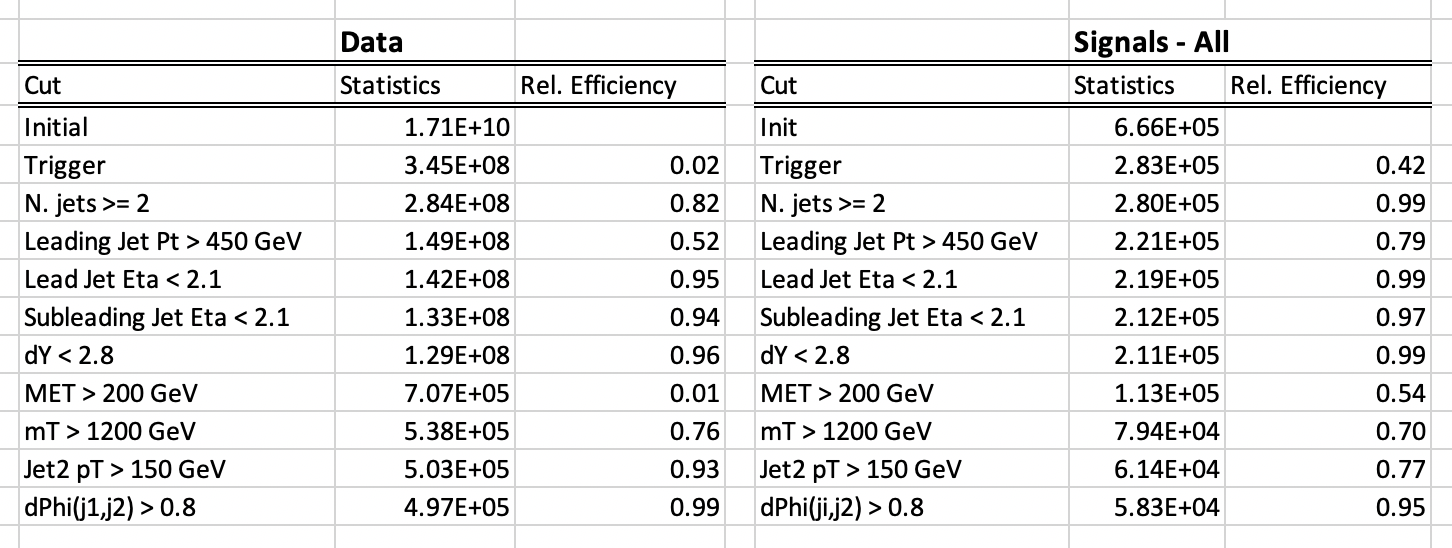
\includegraphics[width=0.95\textwidth]{figures/eventsel/preselection/presel_cutflow}
    \caption{Preselection cuts for data (left) and signal (right).
    \label{fig:presel_cutflow}}
\end{table}

With the exception of the cuts necessary to reduce the non-collision background, all cuts were verified to enhance signal sensitivity by improving $s/\sqrt{b}$, a standard estimate of discovery sensitivity, where $s$ is the number of signal events and $b$ is the number of background events. The cuts on $\Delta$Y and \met~were optimized to enhance $s/\sqrt{b}$, and the other cuts were informed by the physics motivations provided above. \par

Vetos are applied to reject any events where an error for a subdetector is flagged. 
To reject non-collision backgrounds (NCB), such as calorimeter noise, beam halo interactions, or cosmic rays, the standard ATLAS event cleaning procedure is applied.
As this analysis is very dependent on \met~associated to jets, the \textsc{Tight}~\cite{tight_loose} event cleaning working point is applied. 
Tight cleaning requires jets to pass a stricter set of quality requirements compared to the \textsc{Loose}~\cite{tight_loose} cleaning option.
Due to the alignment between jets and \met~ for SVJ events, it was found that two additional cuts (indicated above) are needed to remove NCB.
The process for selecting these cuts is presented in Appendix~\ref{app:ncb}. 

The leading and subleading jets in each event are considered the dark quark candidates from the $Z' \rightarrow q_D\bar{q_D}$ decay.  
They are therefore the two jets of greatest interest in the event, and used in the computation of key analysis variables.
This choice was determined through studies of the dark quark trajectory in simulation which determined that the leading and subleading jets are most often aligned with the dark quarks, and therefore most likely to capture the dark quark hadronization.
This study can be found in Appendix~\ref{app:truthstudies}.

Figure~\ref{fig:presel_vars} and Figure~\ref{fig:presel_vars2} show the distribution of signals, data and background MC in several key analysis variables after preselection is applied.
The variables illustrated are:
\begin{itemize}
\item Transverse mass \mt: key analysis variable which reconstructs the $Z'$ mass, as discussed in Section~\ref{sec:mt}.
\item Leading jet \pt: the trigger variable, and a component of \mt. 
\item Subleading jet \pt: dark quark candidate and component of \mt.
\item Missing transverse energy \met (or MET): component of \mt, and an indication of the presence of dark hadrons. All signals are observed to have more \met than the background.
\item $\Delta\phi$(j1, j2): difference in trajectory of the two leading jets, measured in the $\phi$ plane (recall the ATLAS detector geometry of Figure~\ref{fig:ATLASgeometry}). Orientation of the jets is of importance to the ML model as discussed in Section~\ref{sec:input_model}. 
\item $\Delta$Y(j1, j2): difference in trajectory of the two leading jets, measured in the Y plane (recall Figure~\ref{fig:ATLASgeometry} and the definition of rapidity Equation~\ref{eq:rapidity}). The signals are seen to have lower $\Delta$Y(j1, j2) than the background.
\item $\Delta\phi$(j1, \met): the angular separation between the leading jet and the \met. The leading jet is predominantly back-to-back with the \met.
\item $\Delta\phi$(j2, \met): the angular separation between the subleading jet and the \met. The subleading jet is predominantly aligned with the \met, which is a unique feature of this analysis as jets that are closely aligned with \met~are often removed from other ATLAS analyses.
\end{itemize}

\begin{figure}[!htbp]
\centering
    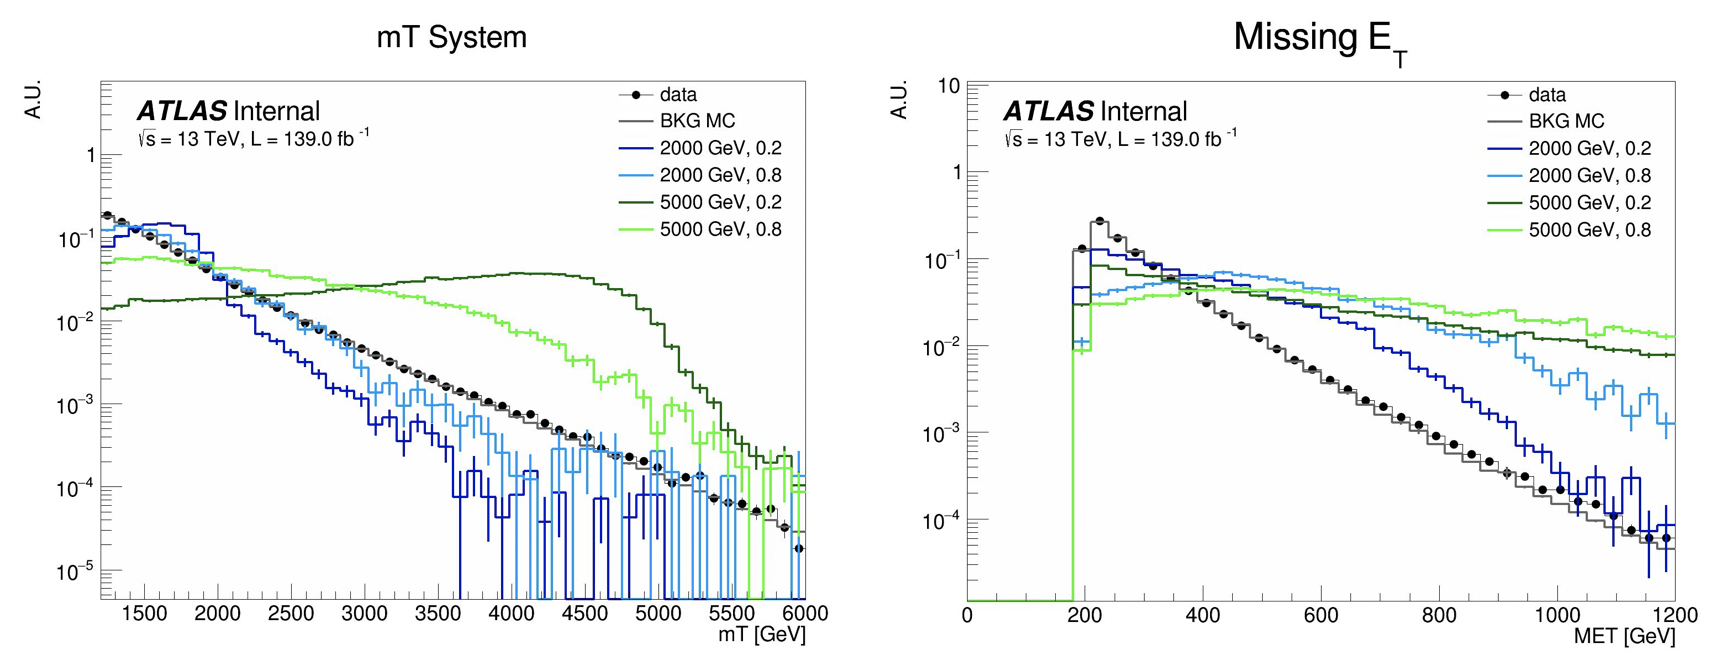
\includegraphics[width=0.95\textwidth]{figures/eventsel/preselection/presel1}
    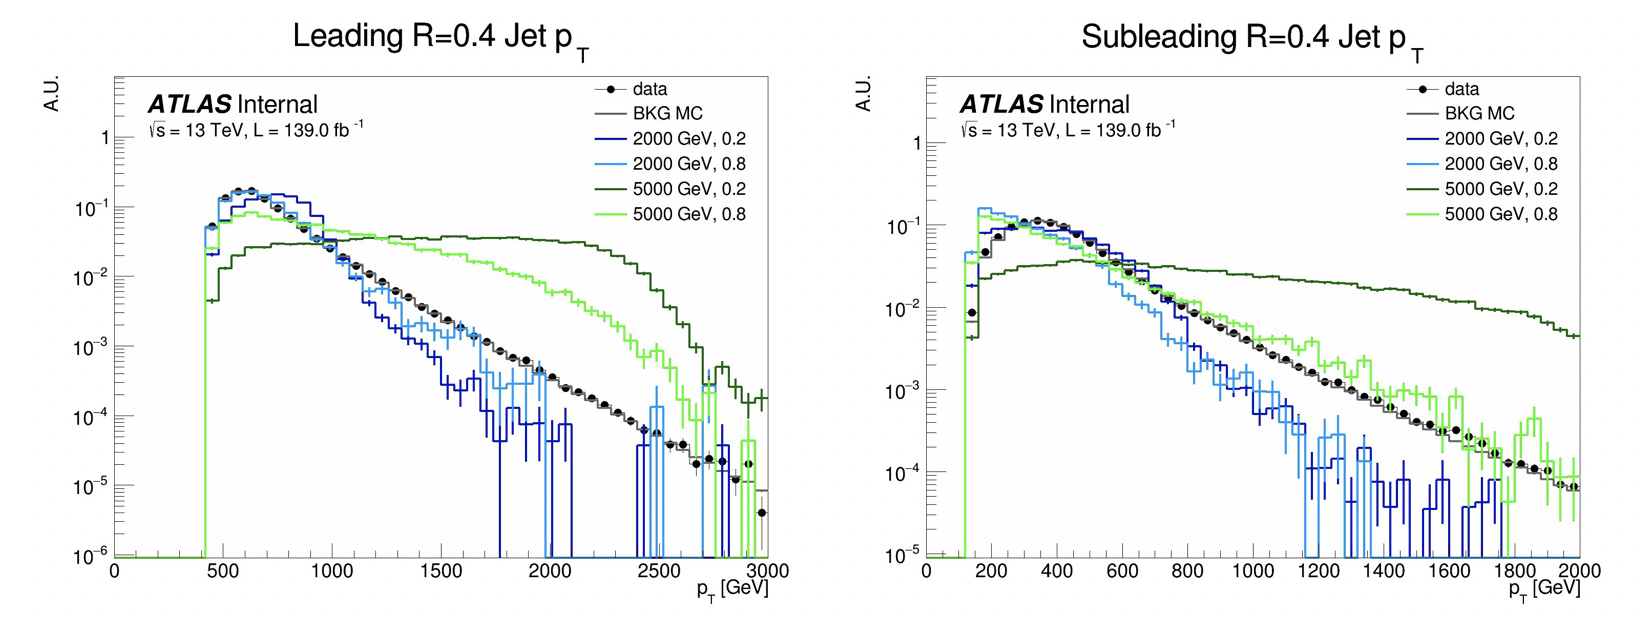
\includegraphics[width=0.95\textwidth]{figures/eventsel/preselection/presel2}
    \caption{Energy and momentum analysis variables at preselection, for data (black), background MC (grey), and representative signal models (color). The signal models are identified in the legend as ``$m_{Z'}$, \rinv''. 
    \label{fig:presel_vars}}
\end{figure}

\begin{figure}[!htbp]
\centering
    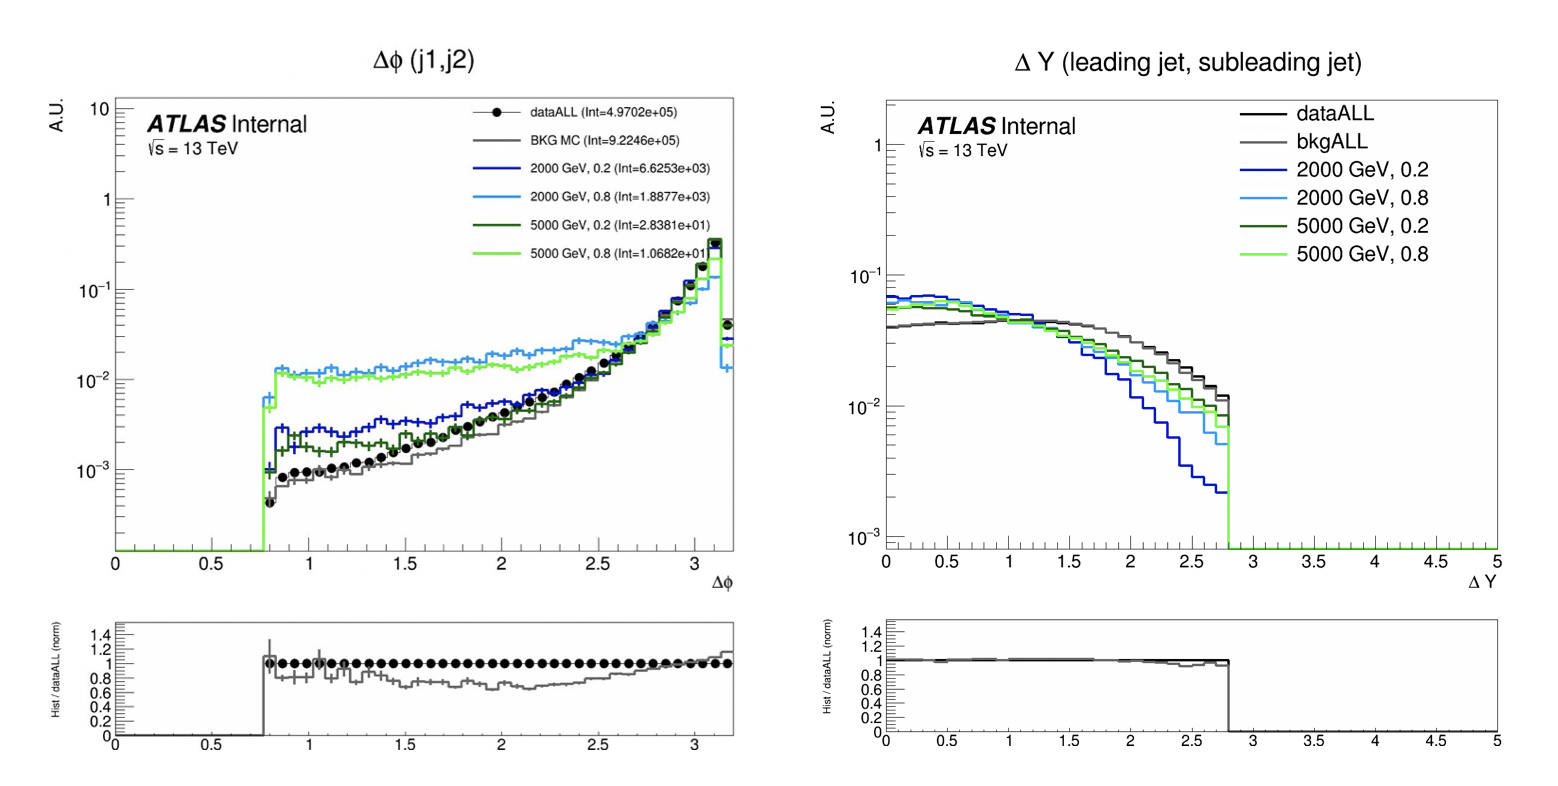
\includegraphics[width=0.95\textwidth]{figures/eventsel/preselection/presel3}
    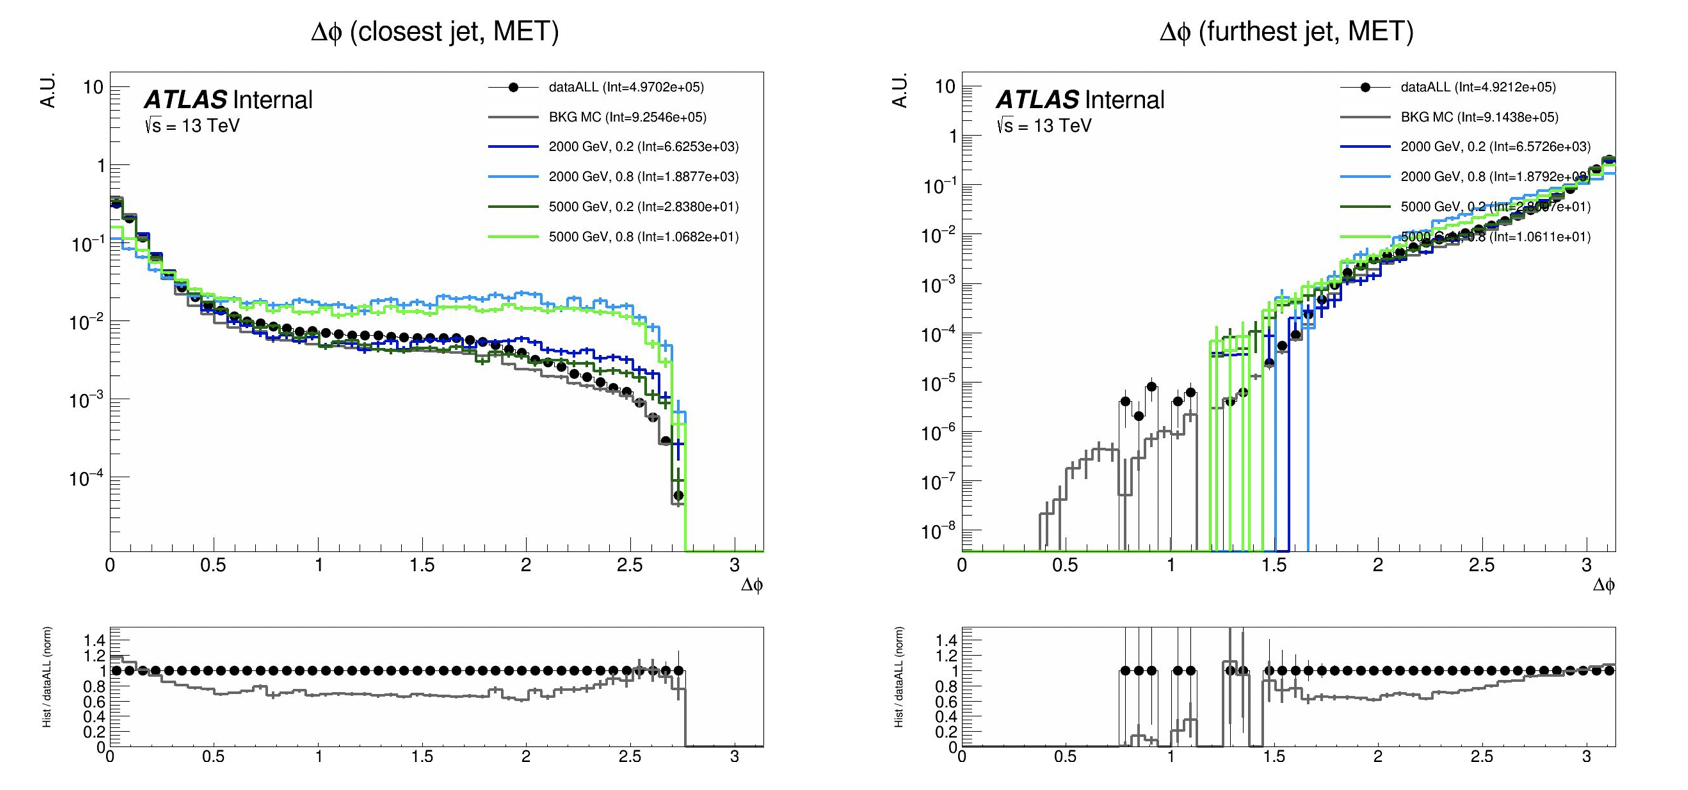
\includegraphics[width=0.95\textwidth]{figures/eventsel/preselection/presel4}
     \caption{Orientation analysis variables at preselection, for data (black), background MC (grey), and representative signal models (color). The signal models are identified in the legend as ``$m_{Z'}$, \rinv''. 
      \label{fig:presel_vars2}}
\end{figure}

The data and background MC are both illustrated in Figure~\ref{fig:presel_vars} and Figure~\ref{fig:presel_vars2}. The agreement between them is generally observed to be good, particularly in the key analysis variable \mt. The agreement is not required to be perfect as the background MC is not used for the background estimation. The primary motivation for studying the background MC is to uncover and remove issues unique to data such as the NCB, as described further in Appendix~\ref{app:ncb}.

 \clearpage
%\input{sections/object}


\section{SVJ Fit and Discovery Analysis Strategies}
\label{sec:strategies}
As was introduced in Chapter~\ref{ch:ml_tools} this analysis is interested in achieving dual goals: to make the best possible measurement of the SVJ signal model generated for this analysis, and to broadly search for any signals consistent with dark QCD behavior and inconsistent with a Standard-Model-only background hypothesis. To this end, two parallel analysis strategies are developed.\par

The SVJ Fit strategy uses the supervised PFN ML score in defining the signal region. Recall, the PFN is trained over simulated MC background and a combination of all MC SVJ signals. This gives this ML tool high sensitivity to the particular nuances of the SVJ shower predicted by the modeled theory. In addition to using the supervised ML tool, the SVJ Fit analysis strategy sets limits on the expected cross section of each signal point in the SVJ signal grid. To achieve this, the shape of the SVJ signals are considered in the final fit, as will be elaborated on Section~\ref{subsec:fit_exclusion}. The combination of the supervised PFN ML score and the signal-shape sensitive fitting strategy allows for the greatest possible sensitivity to the modeled signal process, thus allowing the analysis the best chance at discovery of this model, or enabling the analysis to set the best possible limits on the observed cross section.\par

In contrast, the Discovery analysis strategy attempts to design a more general search, which could be sensitive to SVJs, but also to other possible hidden valley dark QCD models, such as fully dark jets or emerging jets \cite{snowmass}. The Discovery analysis strategy uses the semi-supervised ANTELOPE ML score in defining the signal region. Recall, the ANTELOPE is trained over ATLAS data only, with no explicit knowledge of the SVJ signal behavior. The Discovery fit strategy is also signal model agnostic, by employing a bump hunt \cite{bumphunt} strategy, which searches a smoothly falling template for any bumps inconsistent with a background only hypothesis. Therefore any signal which could present a resonant signature in \mt~could show up as an excess in this strategy. \par

The details of both strategies will be explored in the follow sections which detail the design of the signal regions and fit strategies.
Figure~\ref{fig:fit_strategy} illustrates the difference in the fitting concept.
\begin{figure}[!htbp]
\centering
    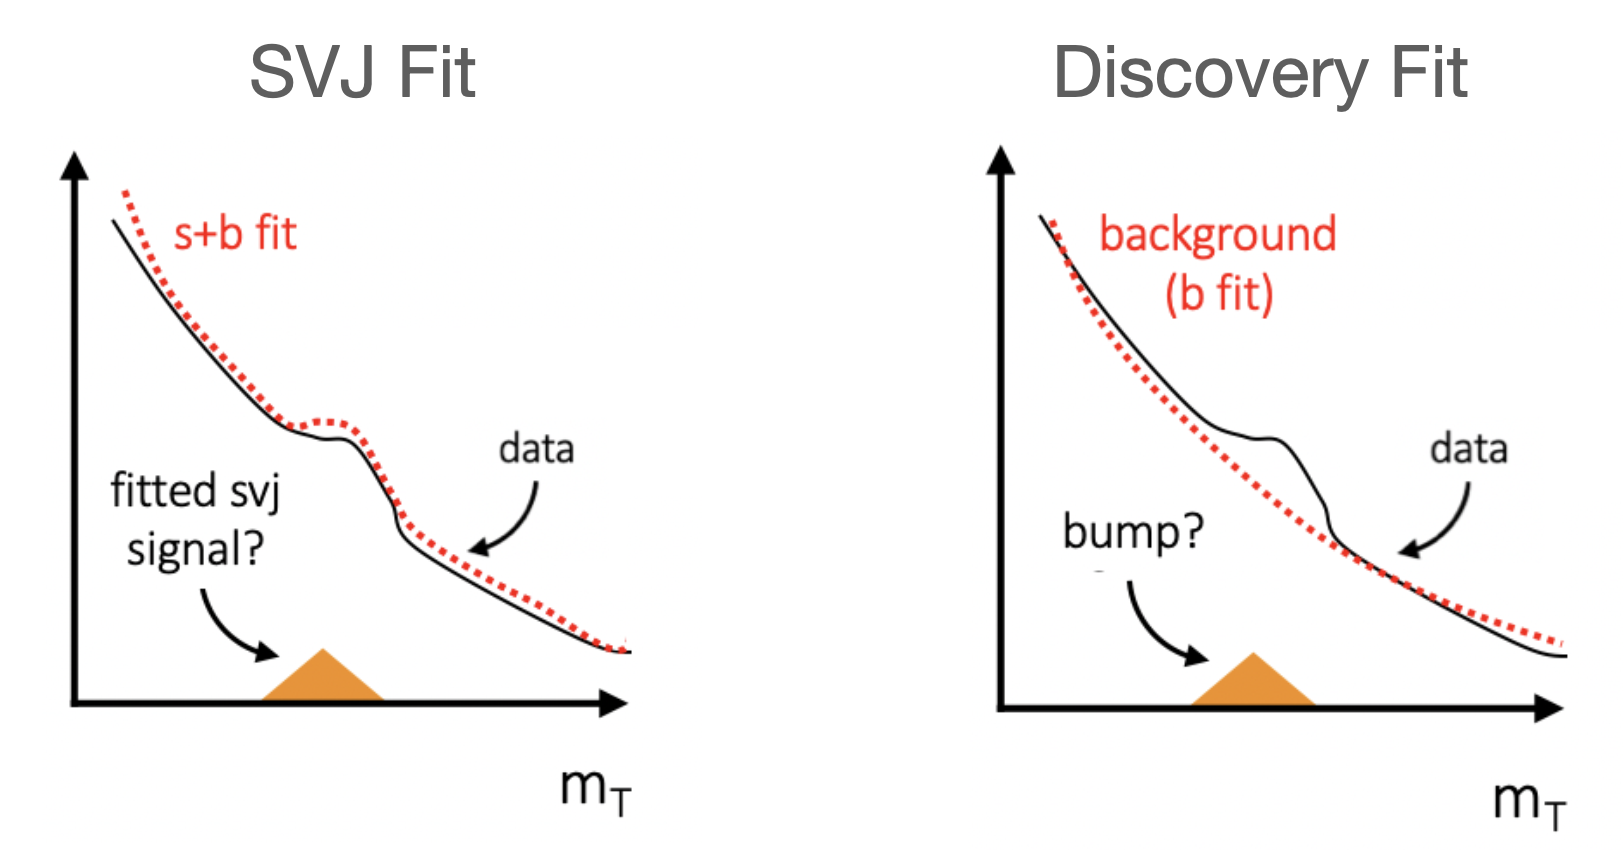
\includegraphics[width=0.5\textwidth]{figures/eventsel/fit_strategy}
    \caption{The two fitting strategies. The SVJ Fit (left) illustrates how SVJ signal shapes will be considered in the fit to search for SVJ specific signal shapes, where ``s+b fit'' indicates a fit that considers the shape of the signal. The Discovery Fit (right) illustrates how the data is compared to a background-only hypothesis to search for any kind of \mt~bump, where ``b fit'' indicates a background-only fit with no signal hypothesis.
    \label{fig:fit_strategy}}
\end{figure}

\section{Analysis Regions}
%------------------------------------------------- 
\subsection{Control and Validation Regions}
\label{subec:sel_crvr}

The final background estimation will come from a polynomial fit to the \mt~distribution in the signal region.
The control and validation regions are needed to develop and test this fit in data.
 
To define the CR selection, a variable is needed that isolates background from all signals across the (\rinv, $m_Z$) grid, which is challenging due to the varying nature of the signal models in quantities such as \met~and \pt~, as illustrated in Figure~\ref{fig:presel_vars}. 
The variable \textit{jet width} is chosen, which is the calorimeter measurement of the spread of the clusters which are used to define the jet ~\cite{jetwidth}.
The concept is illustrated in Figure~\ref{fig:jet2_calo}.
Jets with only one very energetic cluster have a small width, while jets with many lower energy clusters have a large width.
\begin{figure}[!htbp]
\centering
   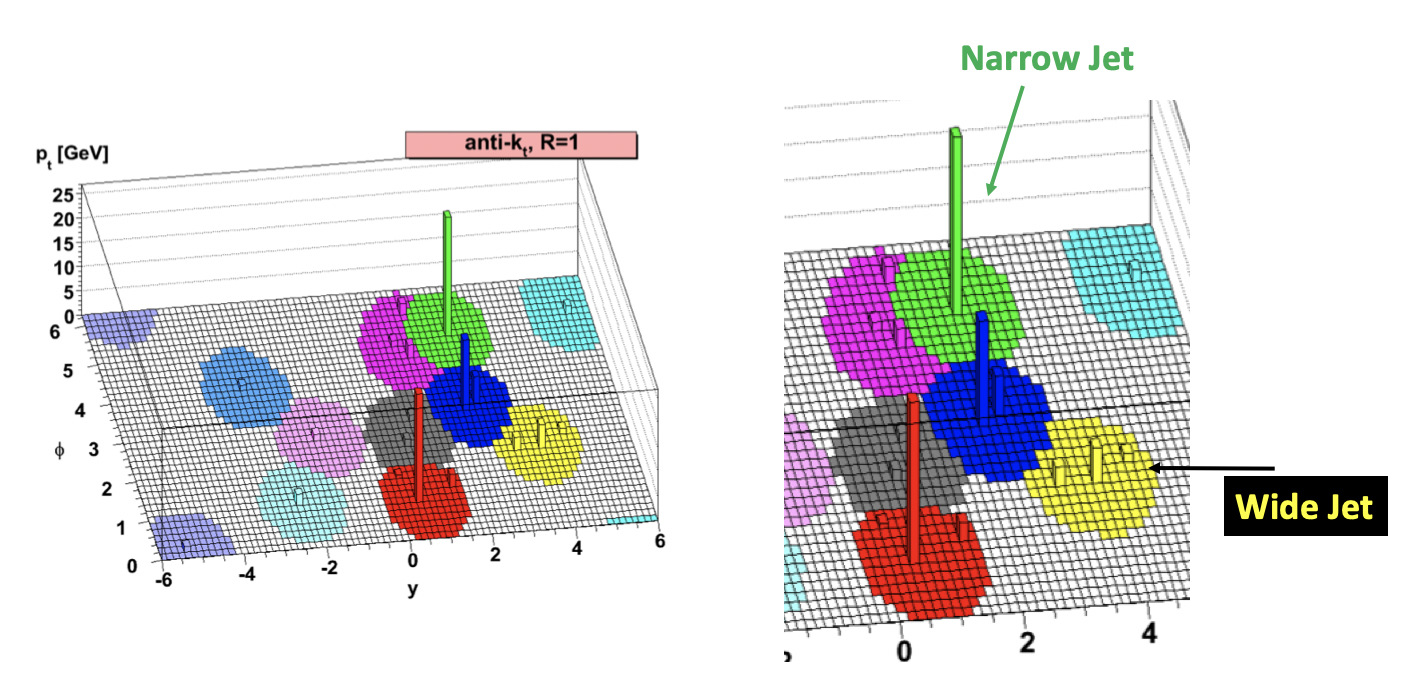
\includegraphics[width=0.95\textwidth]{figures/eventsel/jet2_calo}
    \caption{Recall the construction of anti-$k_t$ jets as described in Section~\ref{sec:jet_cluster} and illustrated in Figure~\ref{fig:jet_algorithms}. On the right, we zoom in on two jets, illustrating the narrow cluster pattern in the green jet, and the wide cluster pattern in the yellow jet.
    \label{fig:jet2_calo}}
\end{figure}

Figure~\ref{fig:jet2width} shows jet width specifically for the subleading jet, in data, background MC and signal at preselection.
The leading jet width, which was determined to be less useful for isolating signal from background is also shown.
The subleading jet is more likely to be aligned with \met, which is why the signal jet width is consistently wider in the subleading jet, but not the leading jet.  %, using v12 of the ntuples.
A selection of width$_{j2} <$ 0.05 is chosen for the CR, with the VR and SR therefore having a selection of width$_{j2}$ $\geq$ 0.05.
 
\begin{figure}[!htbp]
\centering
   %\includegraphics[width=0.4\textwidth]{figures/background/width$_{j2}$_datamc}
   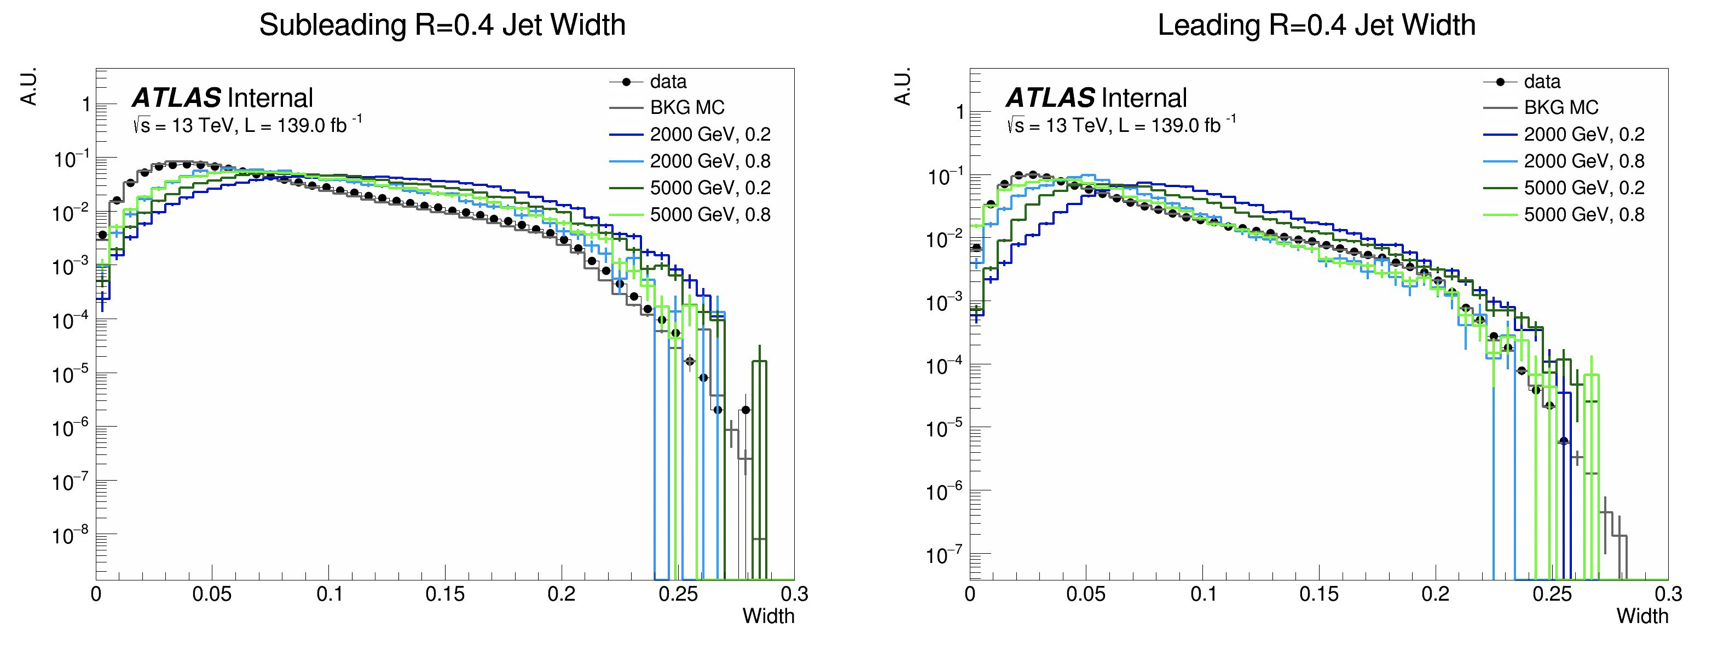
\includegraphics[width=0.98\textwidth]{figures/background/jet2Width}
    \caption{Distributions of the subleading jet width width$_{j2}$ (left) and leading jet width width$_{j1}$ (right) in data, background MC and signals at preselection. All SVJ signals are seen to be wider than the background in width$_{j2}$. The same is not true for width$_{j1}$, where some signals are observed to closely match the background. 
    \label{fig:jet2width}}
\end{figure}

While the CR was used to develop the polynomial strategy, and is the primary region used in many of the fit studies, a validation region is used as an additional check of the estimation strategy in data.
The VR is defined using the region of events with low ML score by either the PFN or ANTELOPE networks.
Here the analysis strategy splits into the two parallel strategies presented in Section~\ref{sec:strategies}: the SVJ fit strategy and the Discovery strategy.
A selection of [PFN score $\leq$ 0.6 \& width$_{j2}$ $\geq$ 0.05] defines the SVJ Fit VR, while [ANTELOPE score $\leq$ 0.7 \& width$_{j2}$ $\geq$ 0.05] defines the discovery VR. 

There are therefore three variables that are crucial to the analysis strategy: width$_{j2}$, ML score, and \mt.
%Figure~\ref{fig:bkg_correlations} shows the correlations of all three variables to one another.
%Any outstanding correations are shown in Figure~\ref{fig:crvrsr_mt} to not sculpt the \mt~distribution and only affect its slope, making these variables trustworthy for extrapolation across background/signal regions and final fitting procedures.
%\begin{figure}[!htbp]
%\centering
 %  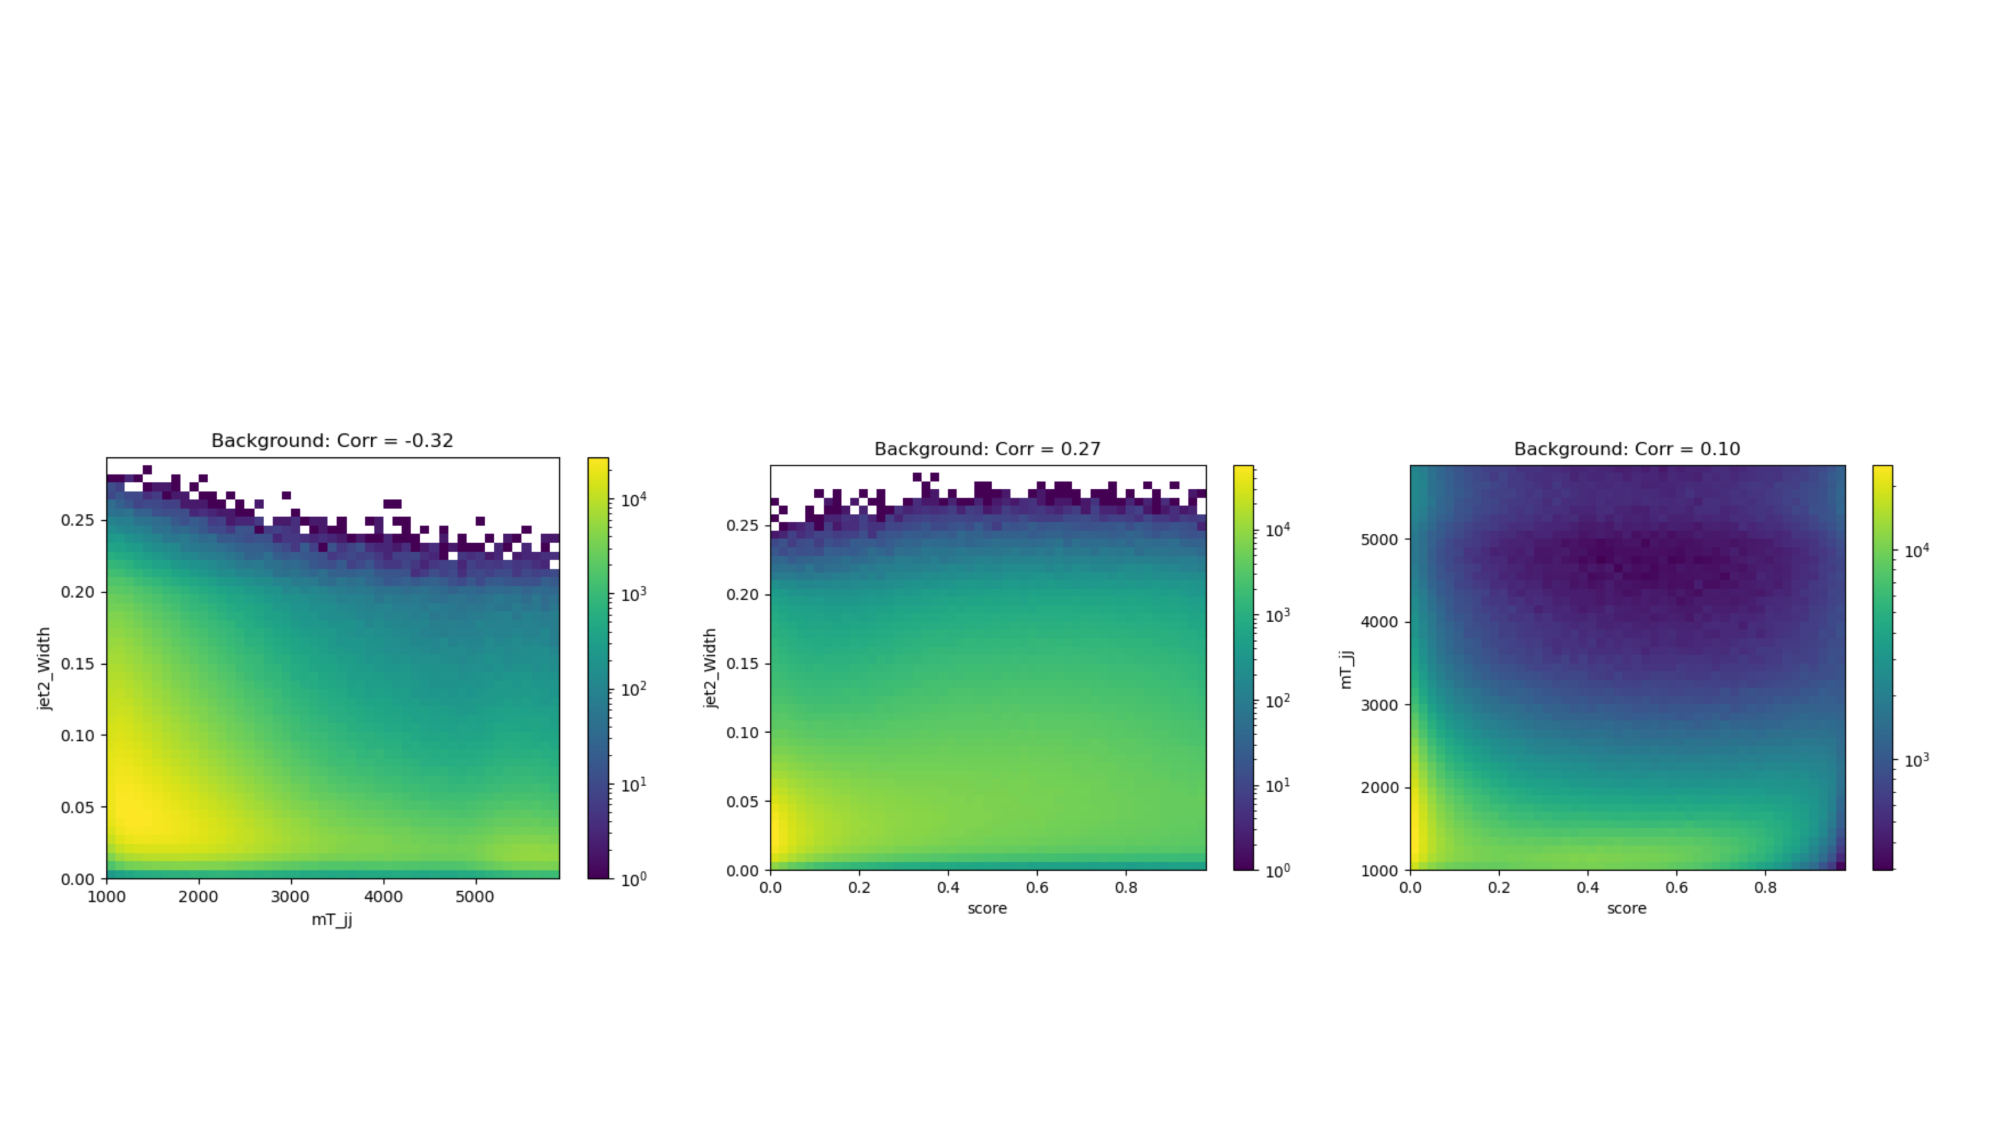
\includegraphics[width=0.95\textwidth]{figures/background/bkg_correlations}
 %  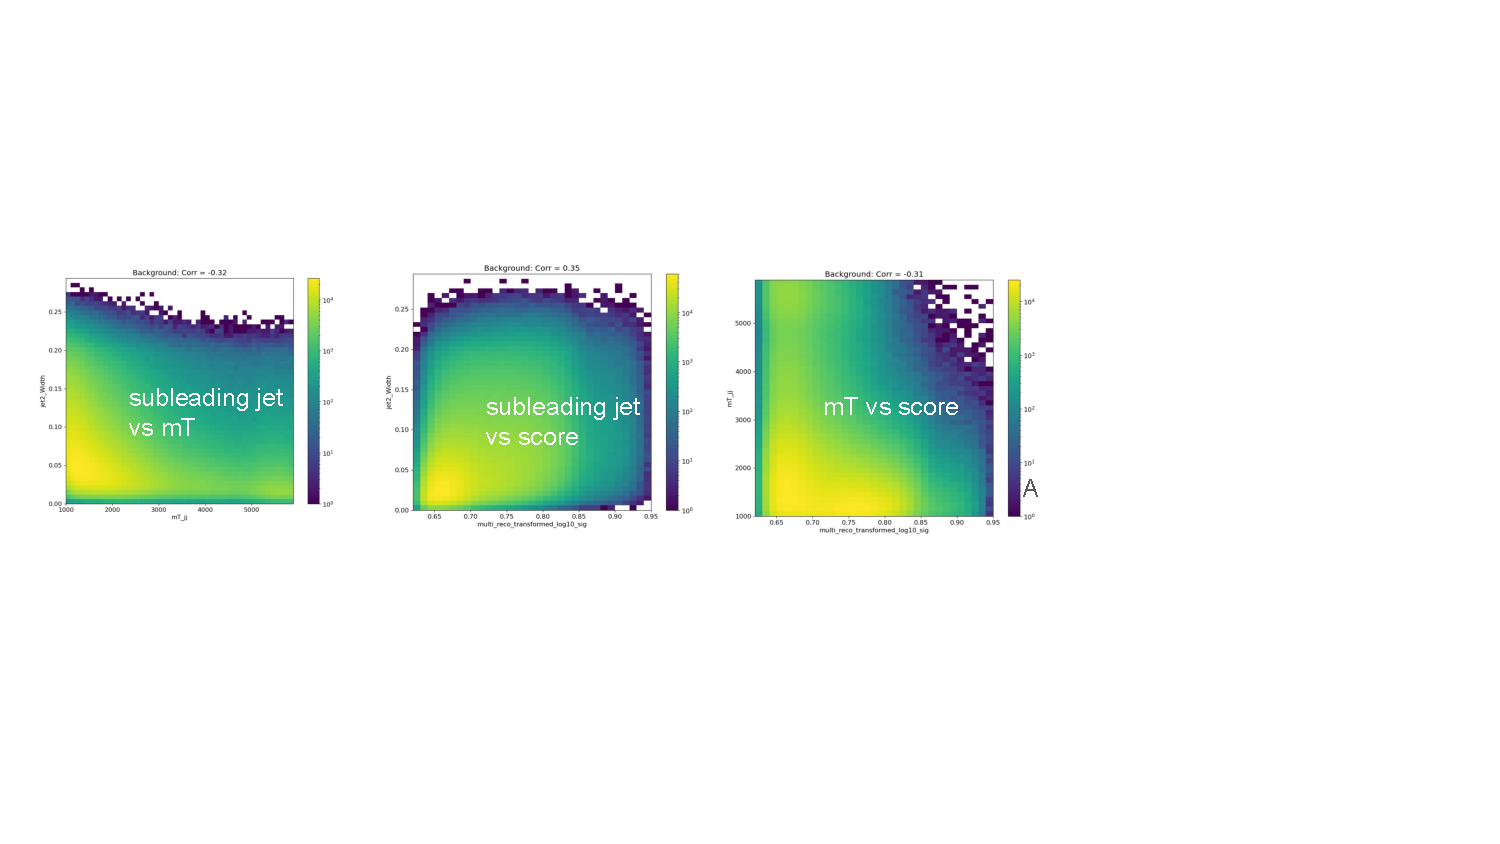
\includegraphics[width=0.95\textwidth]{figures/background/bkg_correlations_antelope}
 %   \caption{2D plots revealing correlations between width$_{j2}$ and \mt~(left), width$_{j2}$ and ML score (middle), and \mt~with ML score (right). For the top row, the ML score is the PFN score, and for the bottom three, the ML score is the ANTELOPE score. Minimal correlations are observed and are shown to not sculpt \mt, validating these variables for analysis region construction and statistical treatment.
%    \label{fig:bkg_correlations}}
%\end{figure}
We check the expected shape of \mt~across the CR, VR, and SR using background MC to ensure the shape is smoothly falling across all 3 regions.
Figure~\ref{fig:crvrsr_mt} shows the distribution of \mt~across the CR, VR, and SR, for both the PFN (supervised) and ANTELOPE (semi-supervised) strategies.
No significant bumps or sculpting are observed.
Some slope is observed in the ratio of the CR to the VR/SR shapes; however, the chosen background estimation strategy of polynomial fitting is expected to accommodate this slope.
Further, testing the ability of the background polynomial to fit shapes with a variety of slopes increases our confidence in the ability to background polynomial to fit the blinded SR \mt~distribution.%, which could be more problematic for a bump-hunt analysis.
\begin{figure}[!htbp]
\centering
   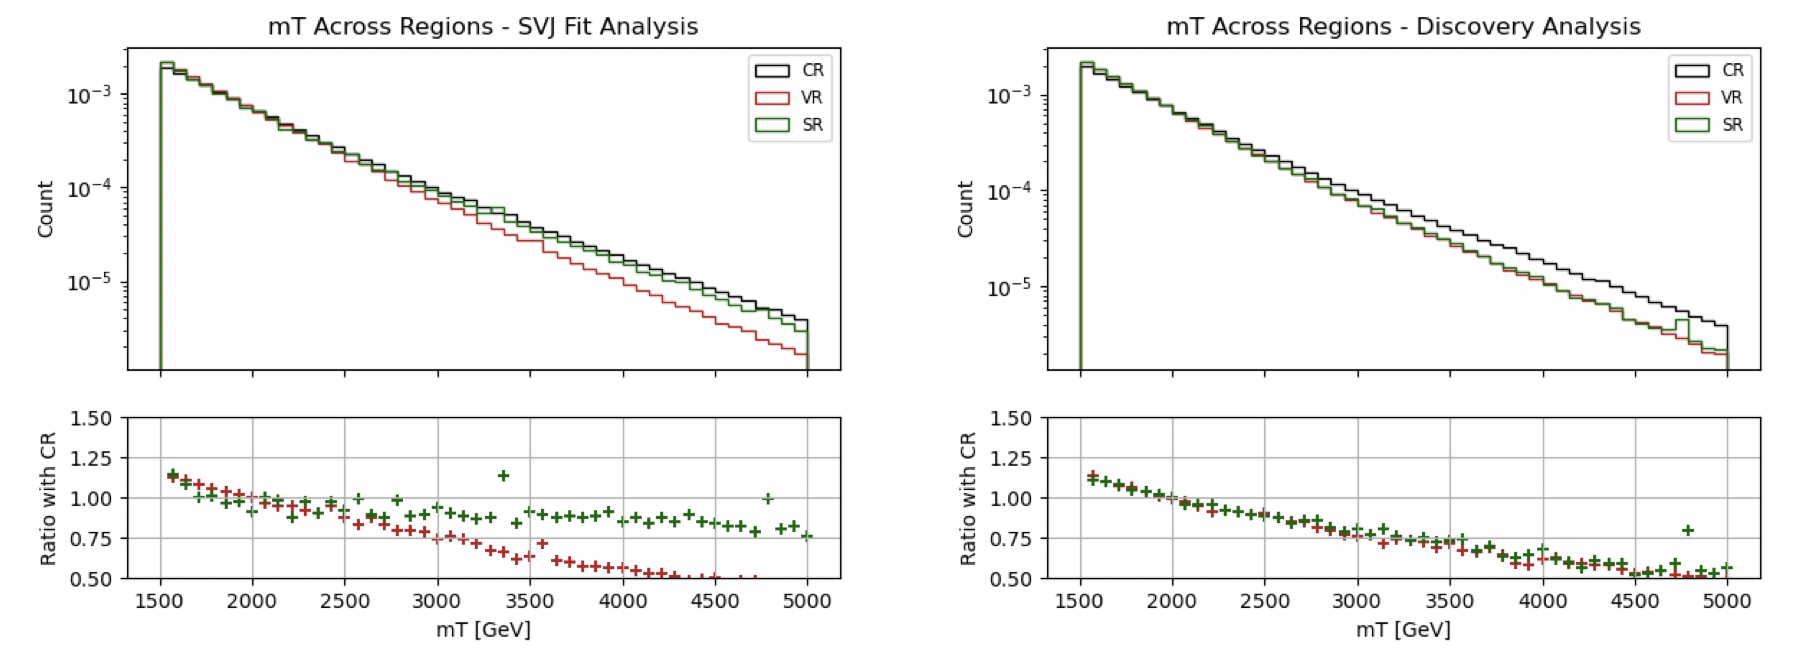
\includegraphics[width=0.98\textwidth]{figures/eventsel/mT_regions}
    \caption{\mt~in simulation across the CR, VR, and SR for both PFN (left) and ANTELOPE (right) selections. While there is variation in the slope of the distribution, no sculpting of bumps is observed.
    \label{fig:crvrsr_mt}}
\end{figure}

%------------------------------------------------- 
\subsection{Signal Region}
\label{subec:sel_sr}

A selection of PFN score $>$ 0.6 in the SVJ Fit region and ANTELOPE score $>$ 0.7 in the Discovery region is made to provide the primary signal-to-background enrichment, as motivated by Section~\ref{subsec:supervised}.
These values are determined to maximize $s/\sqrt{b}$ in each region.
The additional selection of {width$_{j2}$ $\geq$ 0.05} orthogonalizes the SR to the CR.
Note that the PFN and ANTELOPE regions are not orthogonal; this is because the two analysis flows serve different purposes, their statistical treatments are different, and they will not be combined. 

A summary of the SR, CR, and VR definitions can be seen in Figure~\ref{fig:crvrsr_2d}, along with the relative data statistics in each region.
\begin{figure}[!htbp]
\centering
    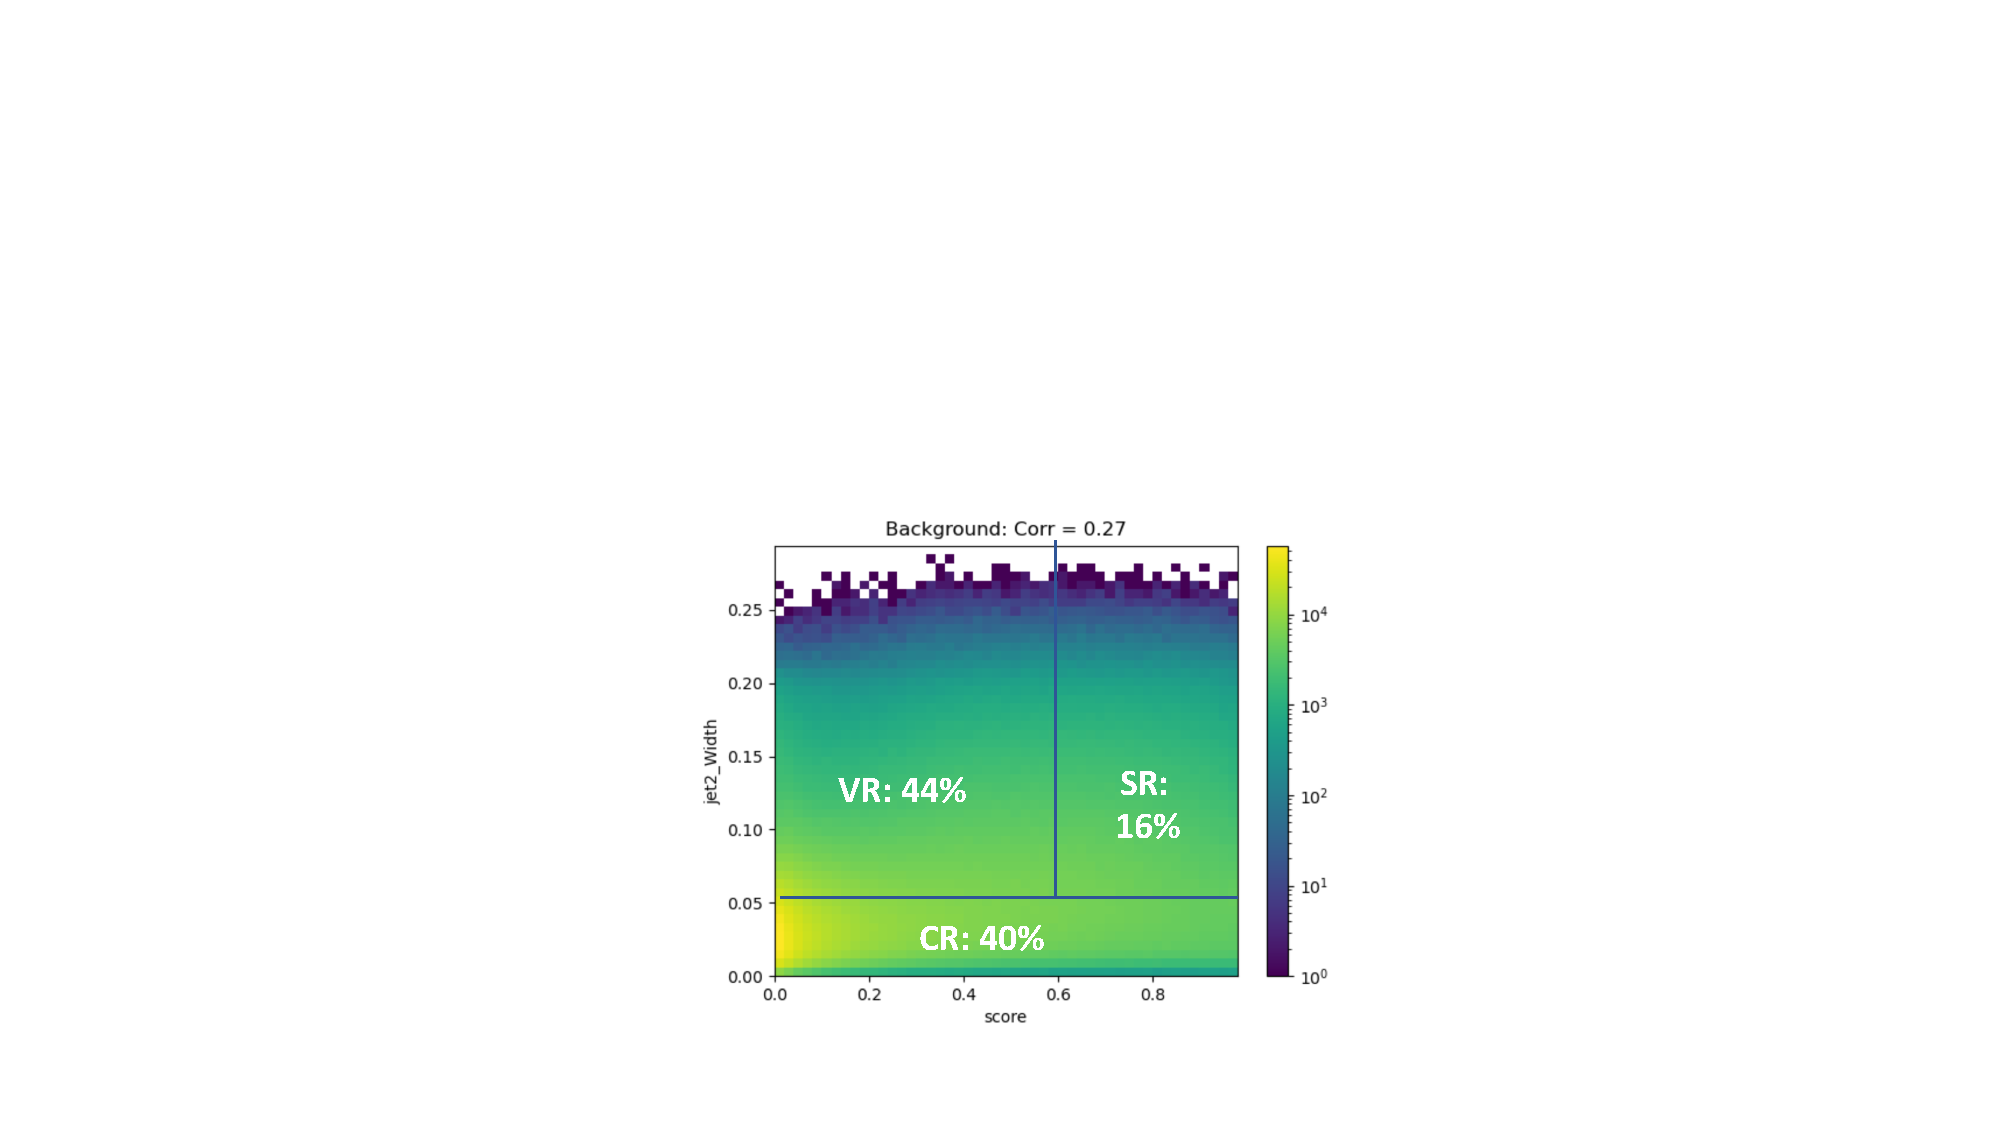
\includegraphics[width=0.98\textwidth]{figures/eventsel/crvrsr_2d}
    \caption{Distribution of data events amongst the CR, VR, and SR regions, along with the fractional population of each region. The SVJ Fit region is shown left with the PFN score on the x-axis, and Discovery region is shown right, with the ANTELOPE score on the x-axis.
    \label{fig:crvrsr_2d}}
\end{figure}

A diagram demonstrating the complete analysis flow can be seen in Figure~\ref{fig:analysisflow}.
\begin{figure}[!htbp]
\centering
    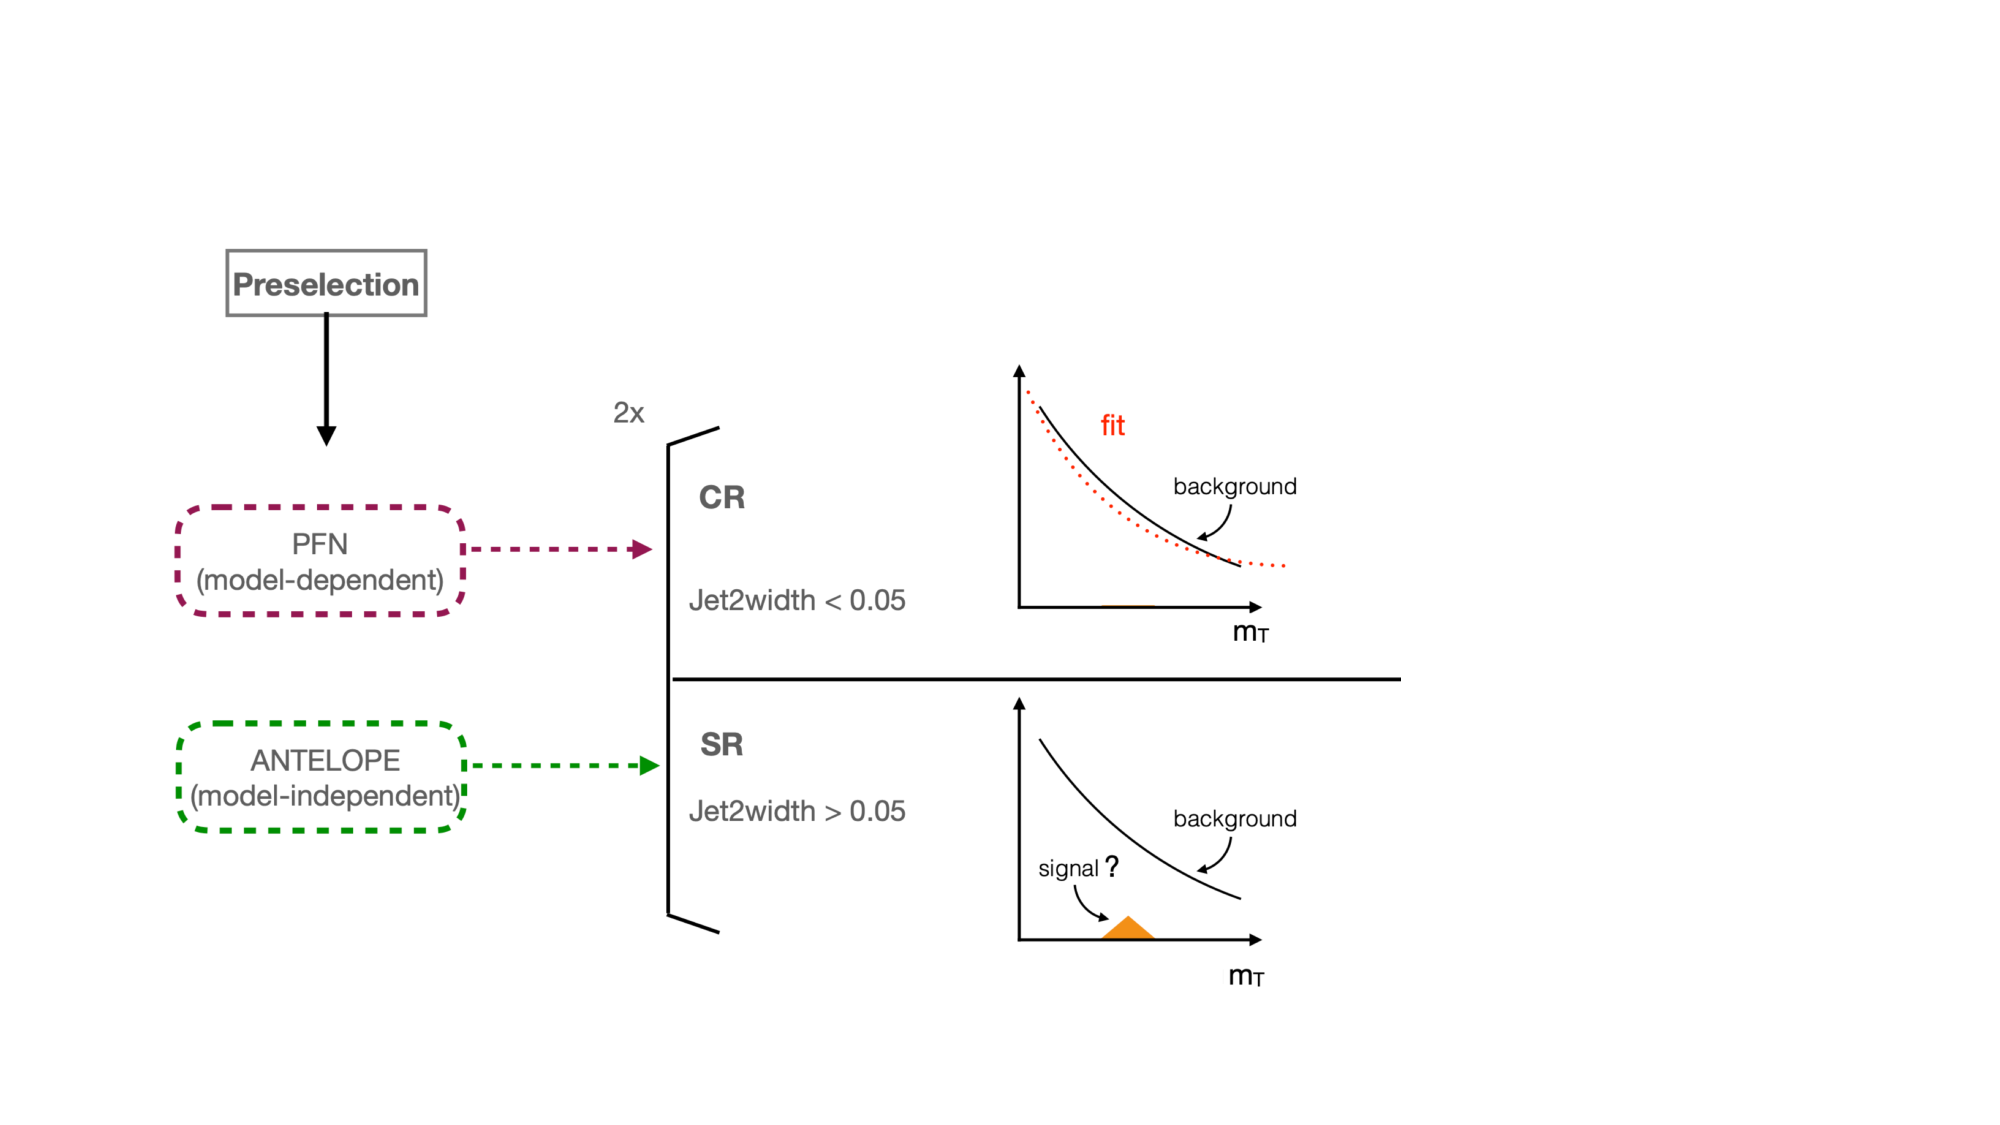
\includegraphics[width=1.1\textwidth]{figures/eventsel/analysisflow}
    \caption{Flow of analysis selections and fitting strategy. From preselection, events with Jet2Width < 0.05 are set aside for the CR. Events with Jet2Width $\geq$ 0.05 are split according the ML score. Events with low ML score create the VR, while events with high ML score create the SR. Events with high PFN score are fitted to determine if they are compatible with the SVJ signal shape. Events with high ANTELOPE score are fitted for a background estimation, and a search for any general data bump is performed.
    \label{fig:analysisflow}}
\end{figure}



\section{Background Estimation}
\label{sec:background}

%Backgrounds: The backgrounds should be evaluated and this should include CR/VR plots with the full data (full run-2 analyses) or at least a representative majority of the data (analyses during data-taking); 
%exceptionally a minor background could be still under finalization, but in this case a short timescale should be envisaged for its completion, or it should be a background that does not affect the accuracy of the result. ( a 10% background on a 10% accuracy measurement is not a minor background)

%This is done via a data template for the shape of \mt~taken from a CR that is orthogonal to the SR, but still close in SM process contribution and kinematic phase space. 
%A polynomial fit is then performed to describe the shape of \mt~in the SR.
%The polynomial is constructed using the CR data template, and validated to data in a VR that is similarly orthogonal to both the CR and SR.
The SM background in the SR is predominantly composed of QCD events, and due to the poor modeling of QCD at high energies by MC, it is estimated in a fully data-driven way. 
An empirical functional form is used for the background shape of \mt.
The ability of this function to model the background behavior is tested both the CR and the VR for each analysis strategy. The shape parameters are left free in all the fits.

The fits are performed for 1500 GeV $<$ \mt~ $<$ 6000 GeV.
The polynomial chosen is a standard 5-parameter function used in several similar dijet search analyses such as \cite{darkjets} \cite{smooth_bkg} \cite{cms_svj} and shown in Equation~\ref{eq:bkgpoly}:
\begin{equation}
f(x) = p_1(1-x)^{p_2}x^{p_3+p_4 lnx+p_5ln^2x}
\label{eq:bkgpoly}
\end{equation}
Here x = m$_{T}$/$\sqrt{s}$ (transverse mass scaled to the $pp$ collision center of mass energy), and $p_i$ are free parameters.
The fit function is required to be fully positive, and the \mt~distribution is fit to 90 even-width bins.
The resulting fit shape is used as the background estimation for both the SVJ Fit strategy and the Discovery strategy. 
Validation of the fit and its ability to both model the background and detect signal are shown in Section~\ref{sec:fit_strategy}.
Higher order polynomials were also considered, but an F-test was performed and the five parameter function was determined to be adequate and optimal for capturing the shape of the background.








\section{Fit Strategy and Validation}
\label{sec:fit_strategy}

The steps taken to validate the fitting approach for both the SVJ Fit strategy and the Discovery strategy will be outlined in the following sections. The signal region fits which compromise the final result will be presented in Chapter~\ref{ch:results},.

\subsection{SVJ Fit Strategy}
\label{subsec:fit_exclusion}

The ability of the five parameter fit function to capture the shape of the background is studied extensively, using data from the CR and VR. Signal injection tests are performed to determine the ability of the fit to recover and quantify any SVJ signal excess. Finally, estimates of the expected sensitivity are made. 
%Results: An overview of the final fit setup including the final discriminating variables(s), the (SR/CR) regions to be included in the fit and the floating normalization parameters. 
%Some rough first expected limits/discovery sensitivity plots are useful if you have them but not necessary. In this case the binning of the final variable(s) and the systematics smoothing/pruning should be indicated.


%------------------------------------------------- 
\subsubsection{Background Only Fits}
\label{subsec:fit_bkgonly}

Three validations are used for the background fit polynomial: MC across all analysis regions, data in the CR and VR, and pseudo-data in the CR and VR. 

Figure~\ref{fig:bkgfit_mc} shows the ability of this polynomial to fit the smoothly falling \mt~background in simulation across all 3 analysis regions (CR, VR, SR).
The \mt~spectrum is fit in 90 even bins.
These distributions are obtained by downsampling the MC statistics to match the relevant statistics of the data region, in accordance with the MC weights.
The high background-only $p$-value indicates a good fit.
\begin{figure}[!htbp]
\centering
   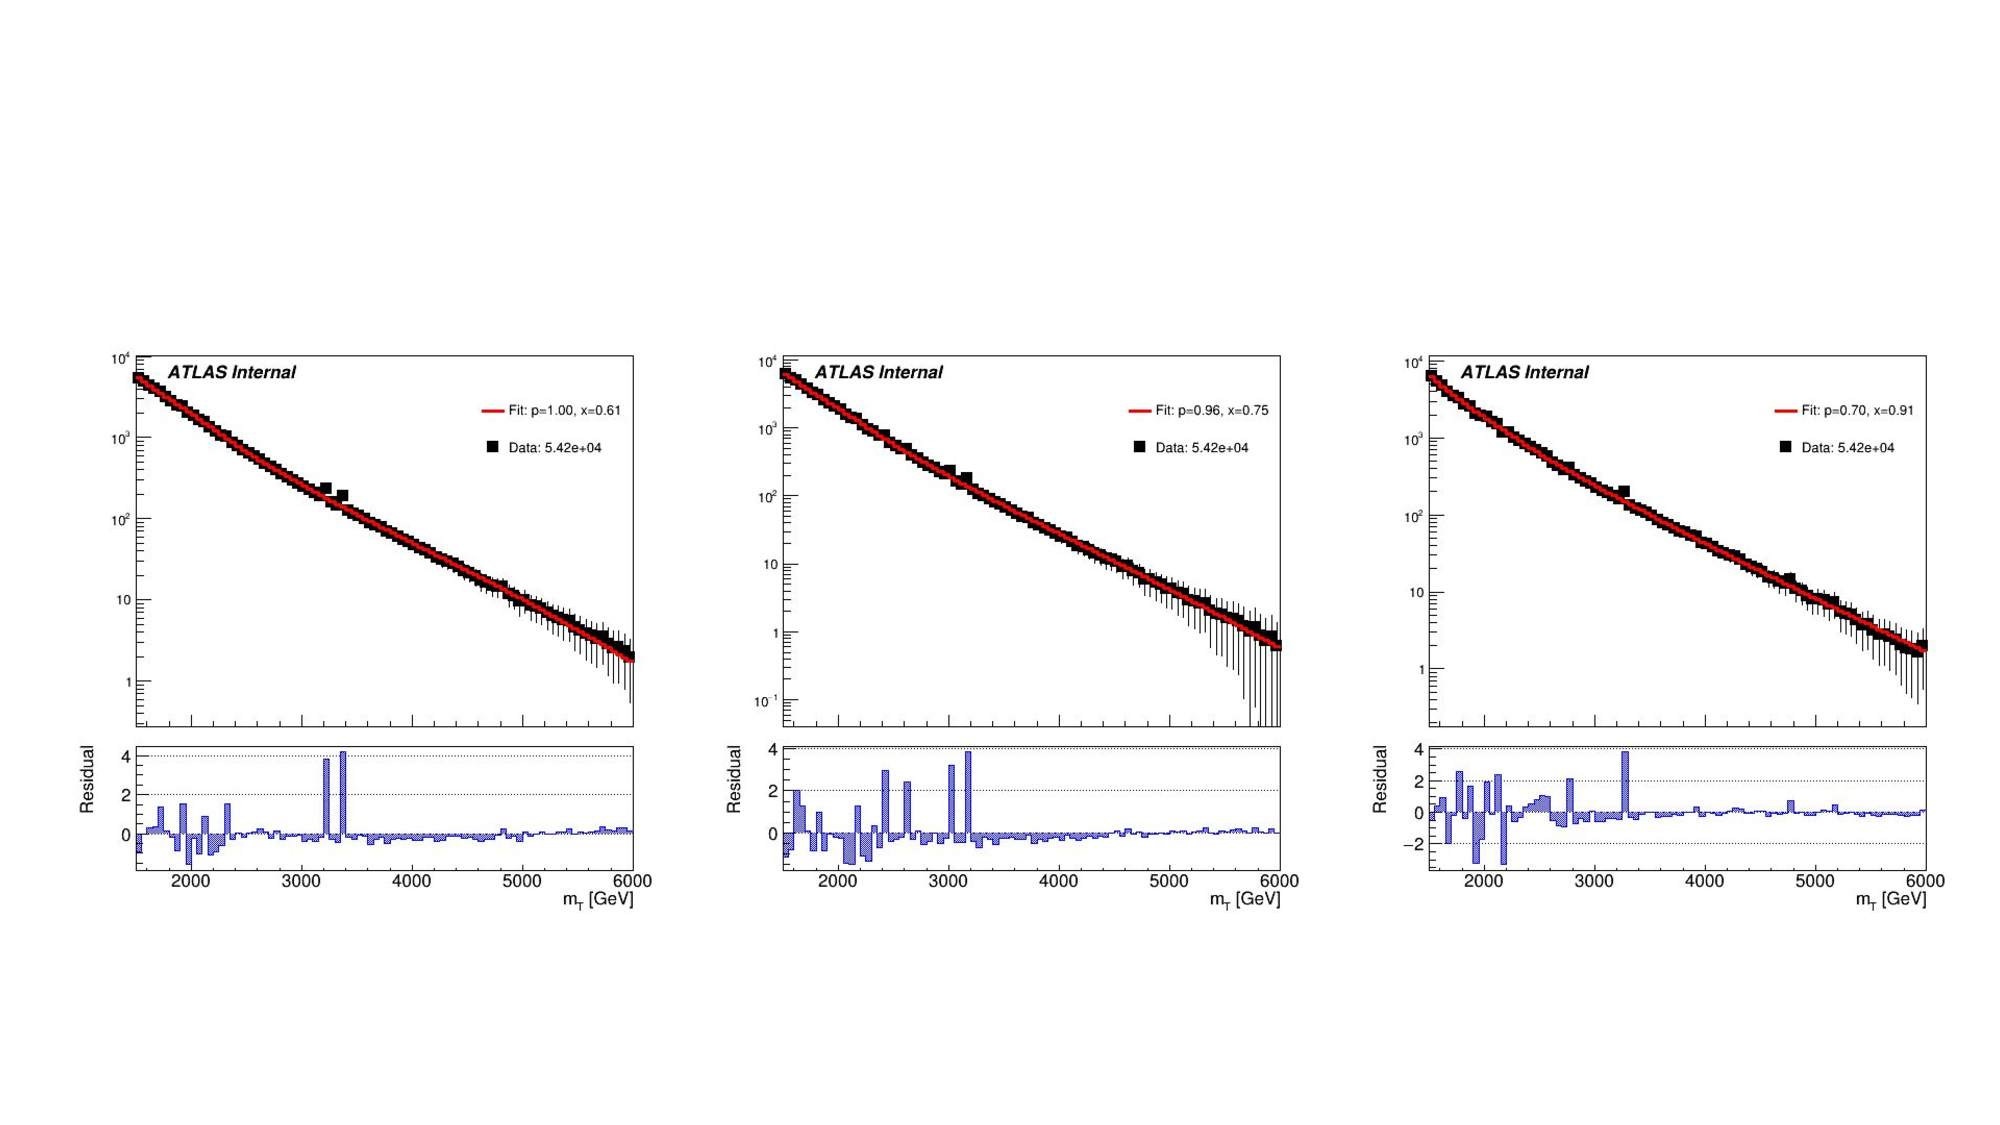
\includegraphics[width=0.95\textwidth]{figures/stats/bkgfit_mc}
    \caption{Background-only \mt~fits using representative MC in the CR (left), VR (middle), and SR (right).
    \label{fig:bkgfit_mc}}
\end{figure}

A slight sinusoidal pattern in the residuals may be observed. 
This arises due to the ``stitching" together of the \pt~slices for the QCD MC (as shown in Figure~\ref{fig:jzslices}), which is picked up by the fit.
For this reason, fitting to MC is only checked to verify that the differences in the slope of \mt~between the three regions (as shown in Figure~\ref{fig:crvrsr_mt}) do not pose a problem for the fitting strategy.

The nature of the functional fitting method allows it to easily adapt to changes in slope of a smoothly falling distribution.
Thus validation of the fit can be performed in data using the CR and the VR distributions to model the expected behavior in the SR. 
Figure~\ref{fig:bkgfit_data_fullstats} shows the a successful fit performed on the full statistics CR and VR regions.
\begin{figure}[!htbp]
\centering
   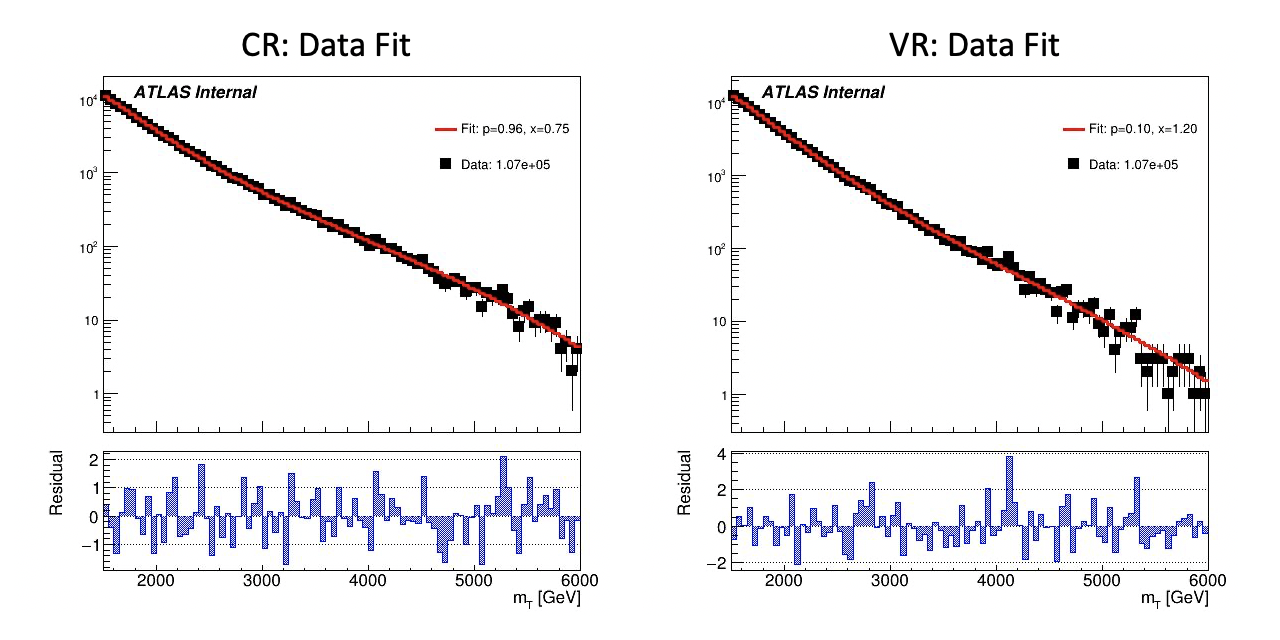
\includegraphics[width=0.82\textwidth]{figures/stats/bkgfit_data_fullstats}
    \caption{Background-only \mt~fits using data in the full statistics CR and VR regions.
    \label{fig:bkgfit_data_fullstats}}
\end{figure}

Figure~\ref{fig:postfit_param_pfn} shows the post-fit values of the fit parameters and their uncertainties for each fit. 
TODO: recalculate so it matches plot
\begin{figure}[!htbp]
\centering
   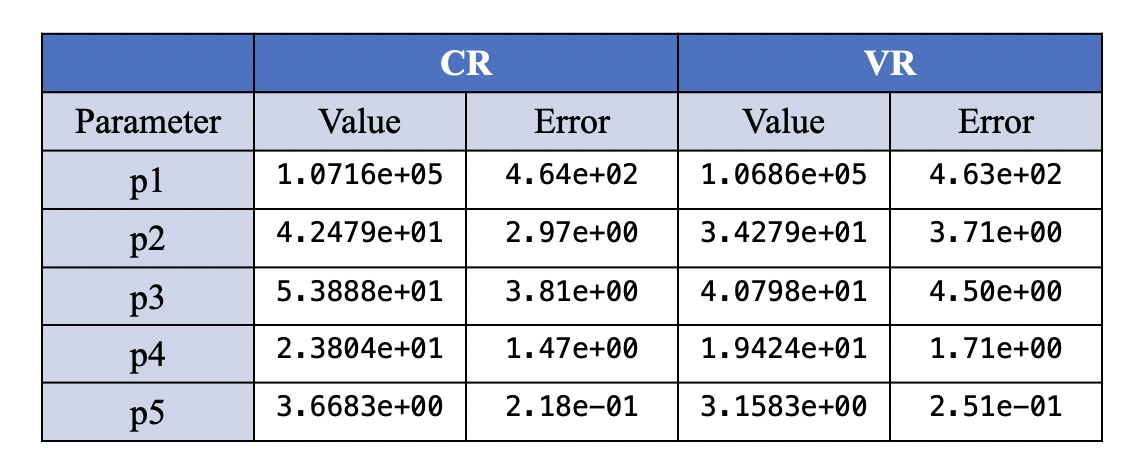
\includegraphics[width=0.65\textwidth]{figures/stats/postfit_param_pfn}
    \caption{Post-fit parameters for the PFN CR and VR.
    \label{fig:postfit_param_pfn}}
\end{figure}


Recall Figure~\ref{fig:crvrsr_2d}, which illustrates that the statistics of the CR and the VR are almost 3x the expected statistics of the SR.
The polynomial fitting strategy is sensitive to the statistics of the fitted template.
Its performance can very substantially depending on the statistical power of the fitted distribution.
To mitigate this, template \mt~histograms are obtained by randomly sampling the data in the CR/VR until a sample that is \textit{statistically identical} to the SR is obtained.
This process is referred to as \textit{downsampling}.
Examples of three downsampled histograms are provided for each region in Figure~\ref{fig:bkgfit_data}.
TODO: recalculate VR see if it's still bad
\begin{figure}[!htbp]
\centering
   %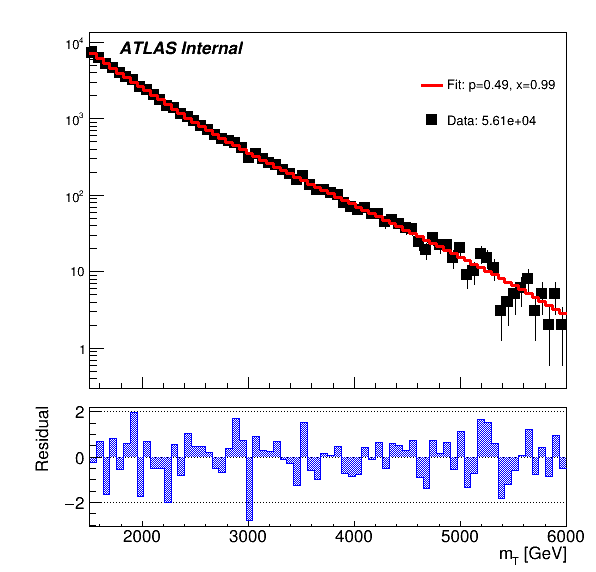
\includegraphics[width=0.32\textwidth]{figures/stats/dataDSfiveParFitChi2_CR0.png}
   %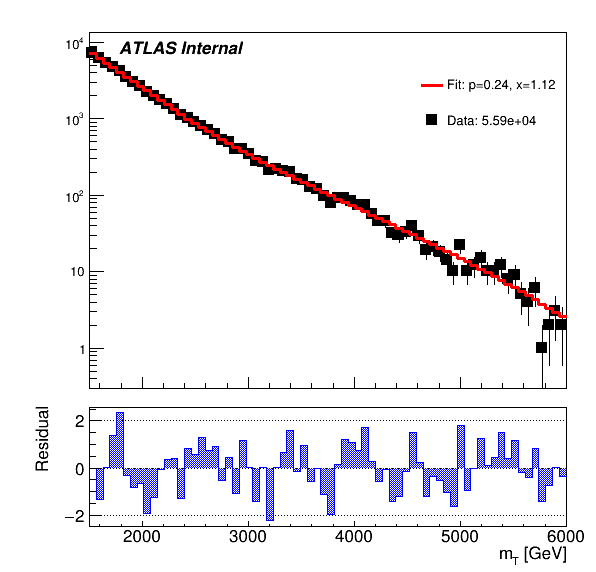
\includegraphics[width=0.32\textwidth]{figures/stats/dataDSfiveParFitChi2_CR1.png}
   %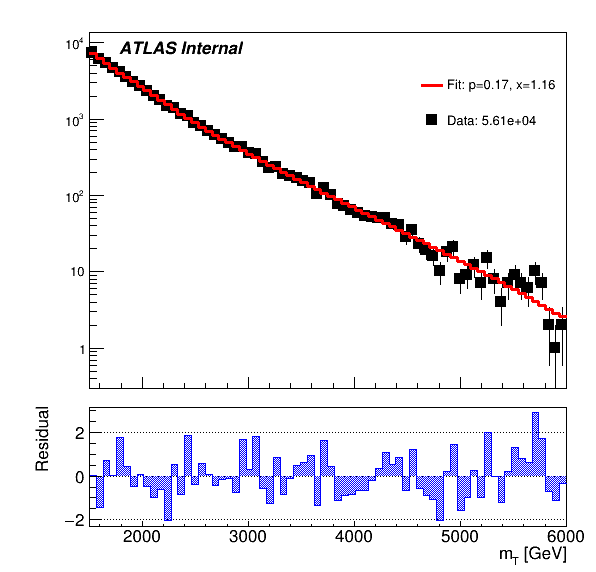
\includegraphics[width=0.32\textwidth]{figures/stats/dataDSfiveParFitChi2_CR2.png}
   %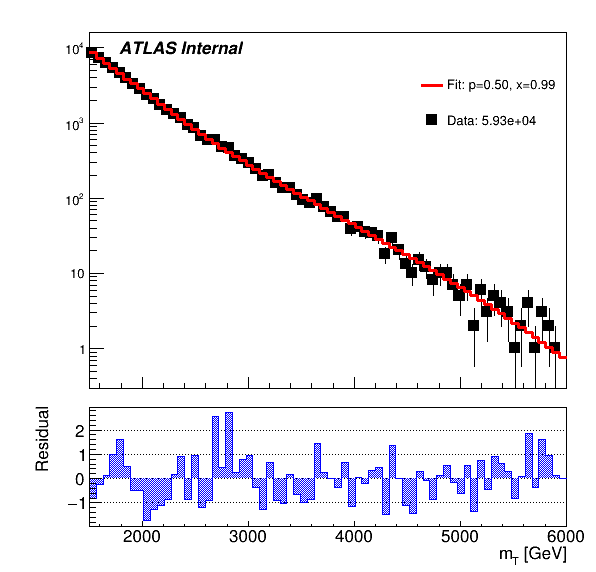
\includegraphics[width=0.32\textwidth]{figures/stats/dataDSfiveParFitChi2_VR0.png}
   %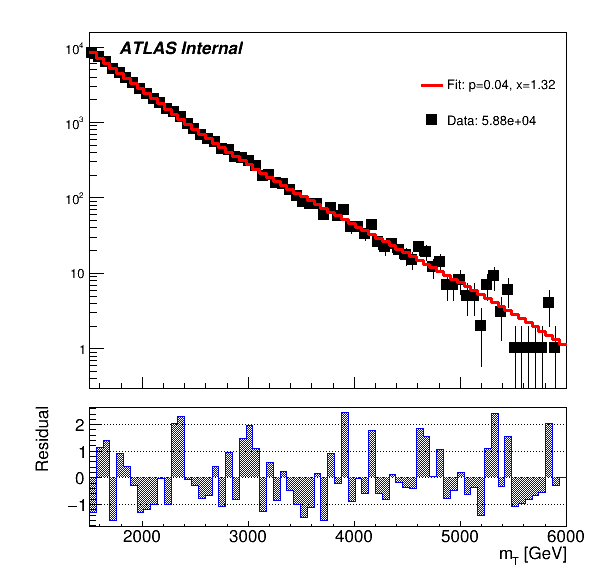
\includegraphics[width=0.32\textwidth]{figures/stats/dataDSfiveParFitChi2_VR1.png}
   %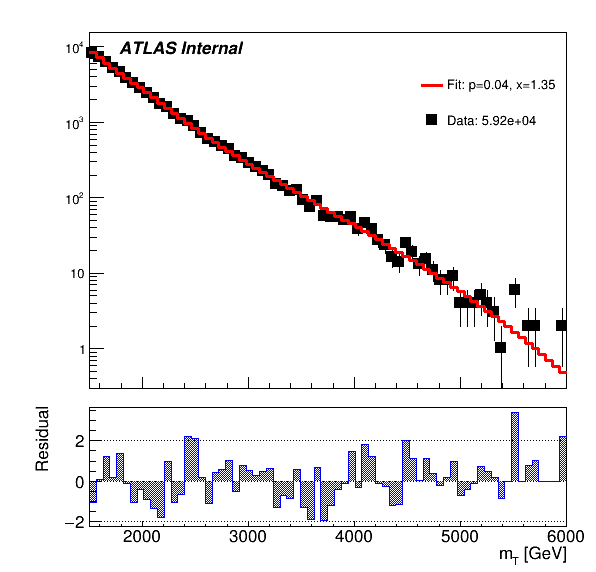
\includegraphics[width=0.32\textwidth]{figures/stats/dataDSfiveParFitChi2_VR2.png}
   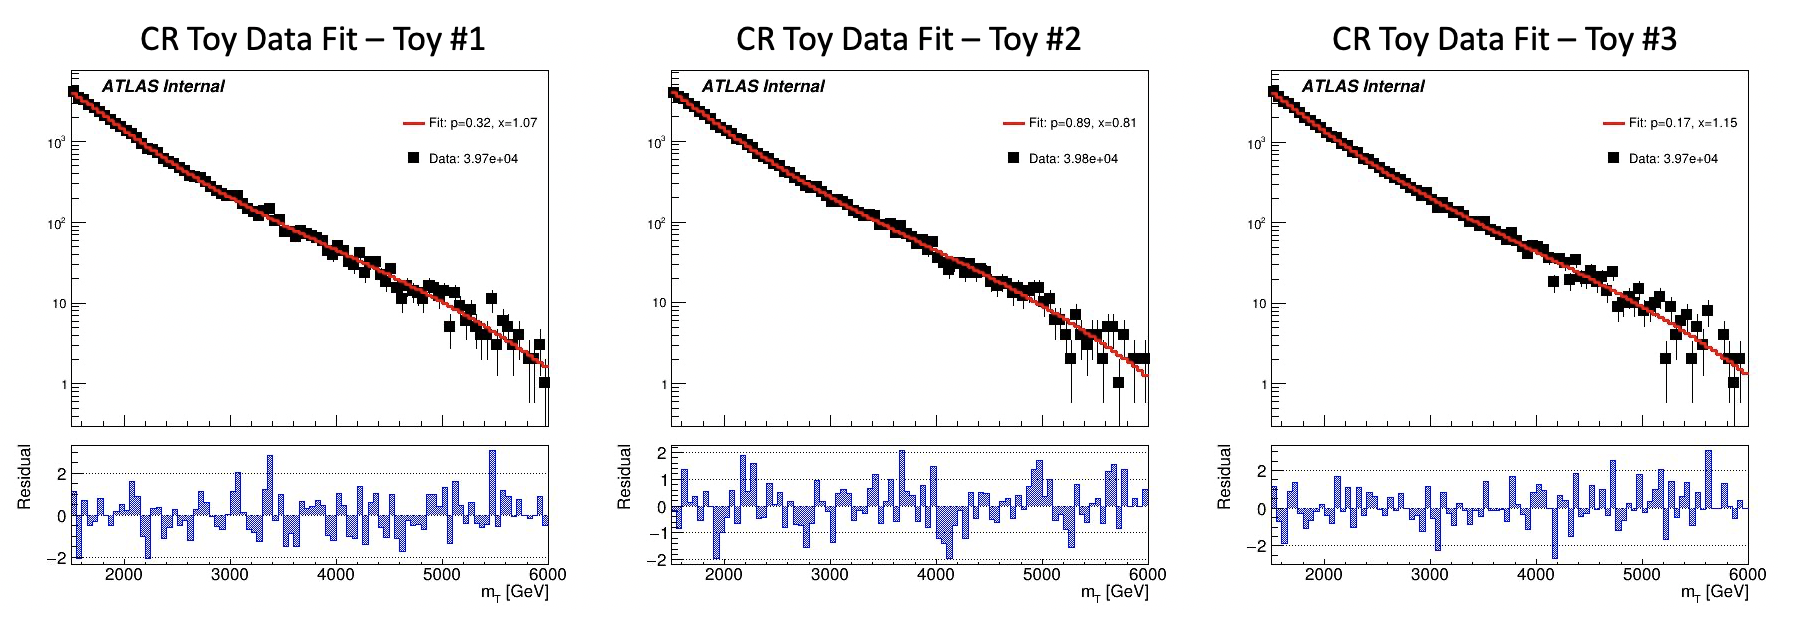
\includegraphics[width=0.92\textwidth]{figures/stats/bkgfit_data_cr}
   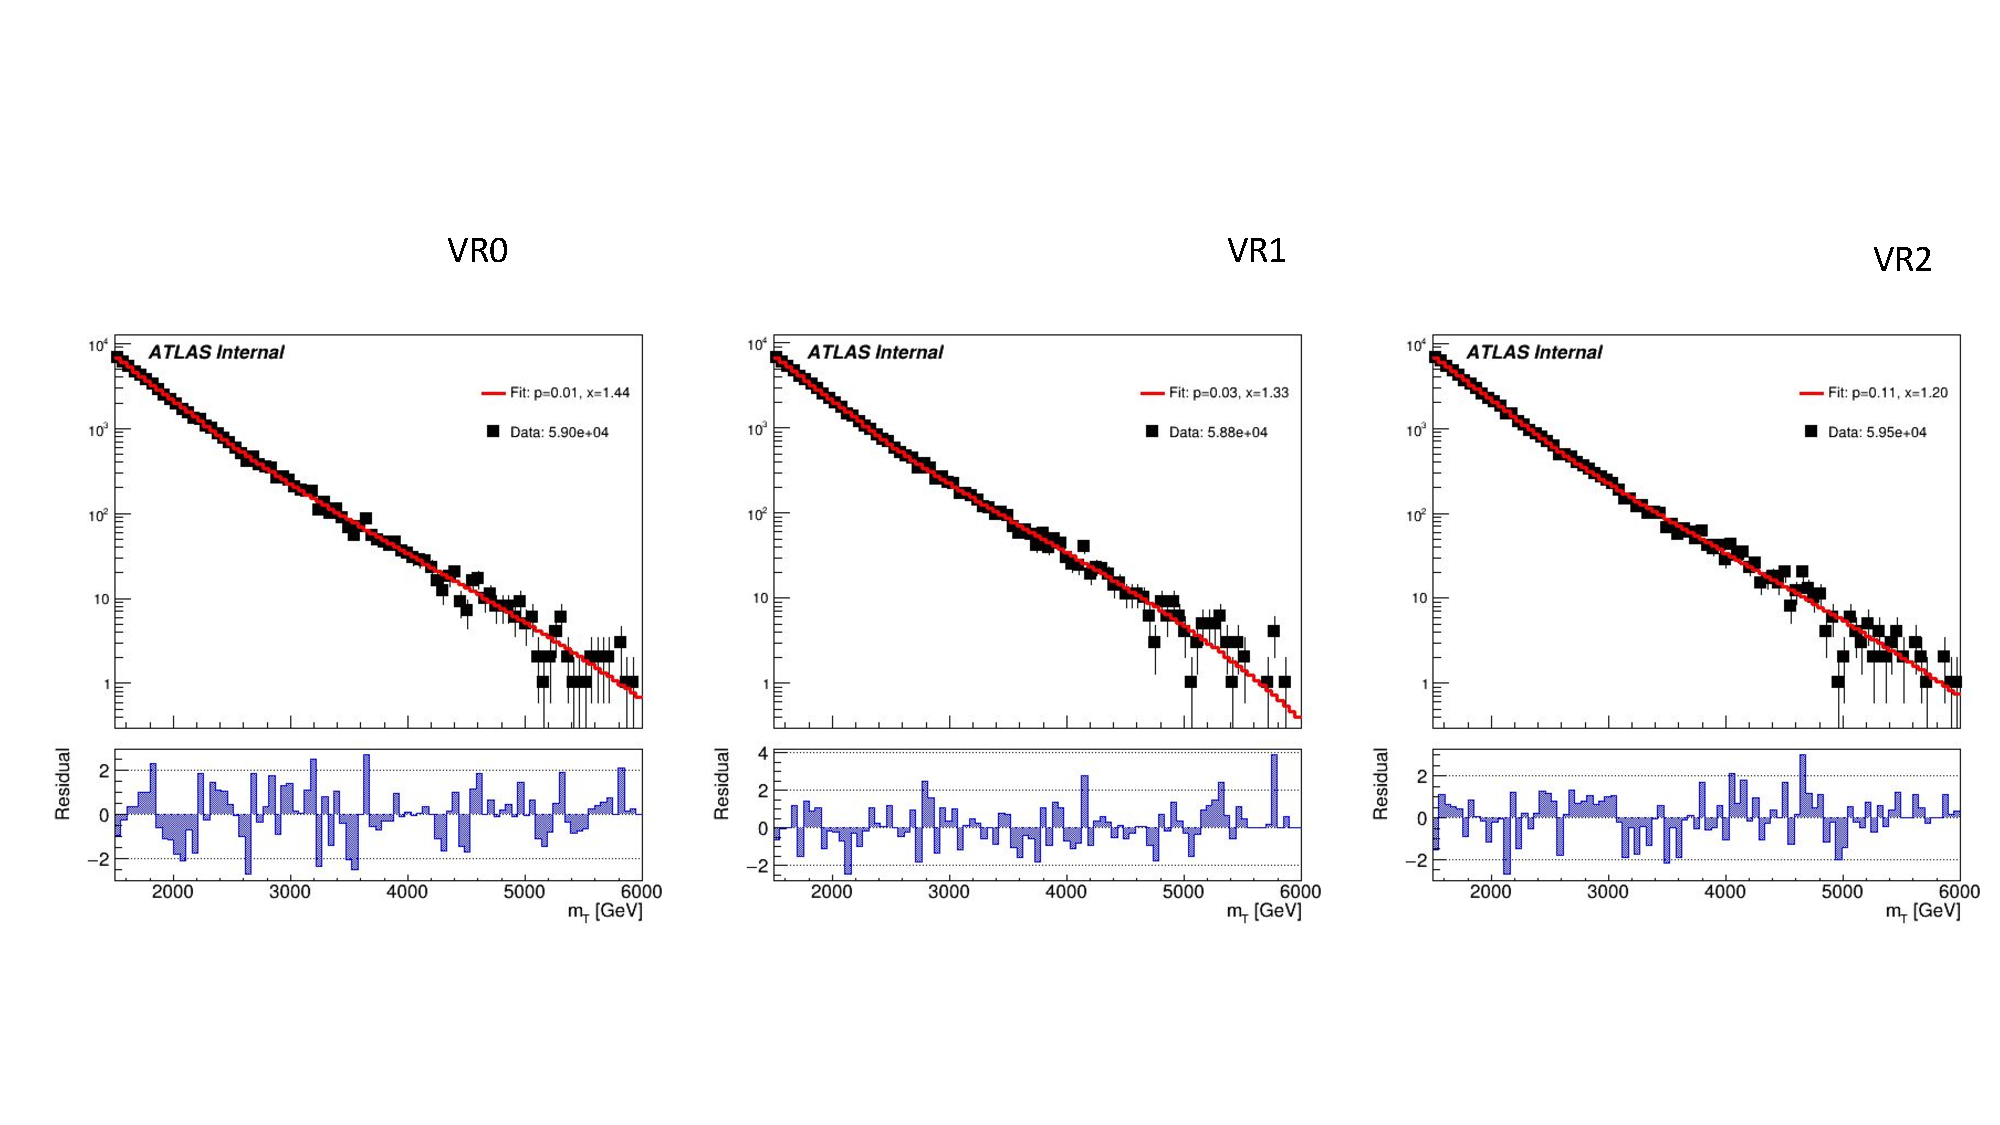
\includegraphics[width=0.92\textwidth]{figures/stats/bkgfit_data_vr}
    \caption{Background-only \mt~fits using data in orthogonal but statistically identical samples to the SR, obtained by downsampling the CR/VR statistics, for the CR (top) and VR (bottom).
    \label{fig:bkgfit_data}}
\end{figure}

To further validate the fit stability of the fit against potential statistical fluctuations, \textit{pseudo-data} (also known as \textit{toy datasets}) are created from the CR data distribution. 
The pseudo-data is created following an \textit{Asimov} prescription \cite{asimov}, using a template to generate a set of toys representing different possible statistical fluctuations.
When studied as a group, the performance of the pseudo-data collection represents the range of possible behavior for an unknown distribution (the SR data in this case), given its statistical uncertainties.
The template used to generate the pseudo-data is a smoothed version of the CR. 
The smoothing applied follows the procedure for functional decomposition described in Ref.~\cite{edgar2018functional}.
Figure~\ref{fig:smoothing} shows the impact of smoothing on the source data distribution in the CR.
Toys are then generated from the smoothed distribution, by varying each bin within its statistical uncertainty according to a Poisson distribution. 
\begin{figure}[!htbp]
\centering
   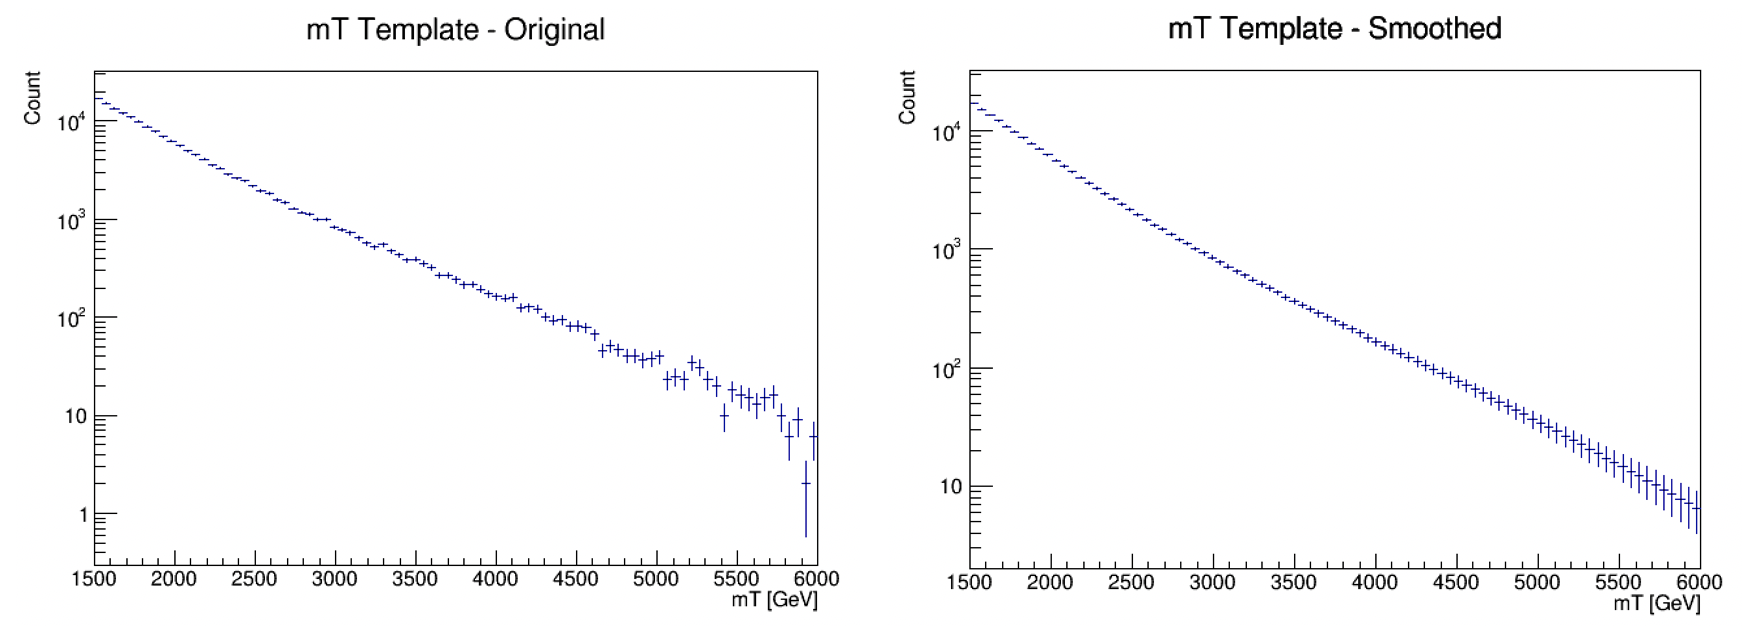
\includegraphics[width=0.85\textwidth]{figures/stats/smoothing}
    \caption{\mt~distribution in the data CR, before (left) and after (right) smoothing.
    \label{fig:smoothing}}
\end{figure}

Figure~\ref{fig:asimov_hist} shows the resulting p-values after an ensemble of 100 Asimov pseudo-data are each individually fit. 
This test determines the likelihood of exceptionally good (high p-value) or poor (low p-value) fits due to randoms statistical fluctuations in the data. 
A flat distribution is observed, indicating good statistical behavior. 
\begin{figure}[!htbp]
\centering
   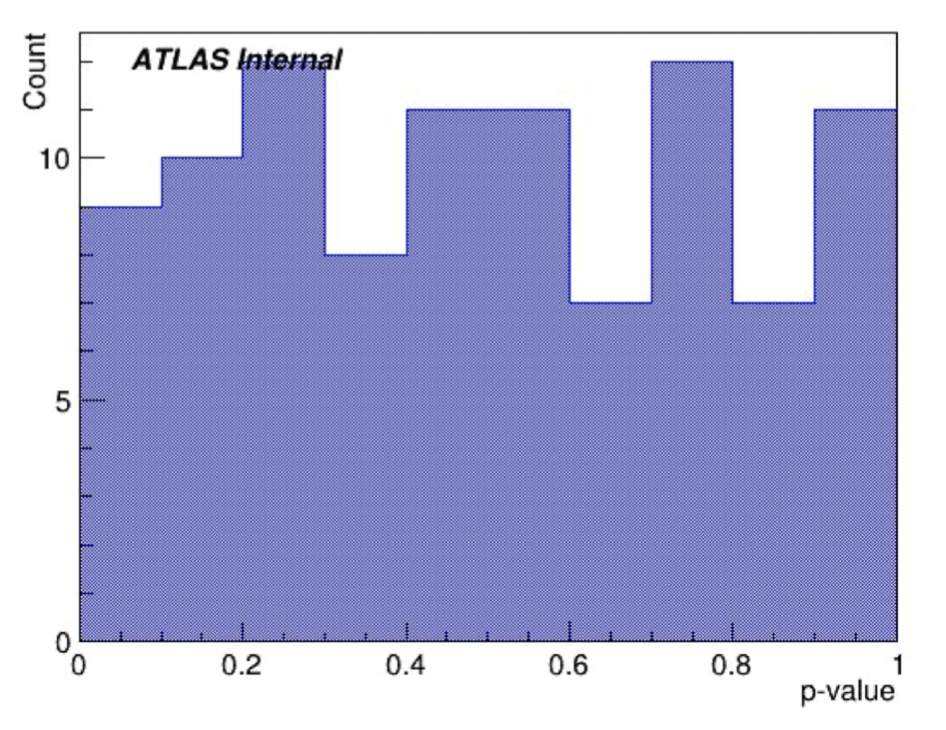
\includegraphics[width=0.45\textwidth]{figures/stats/asimov_cr_hist}
    \caption{$p$-value histograms from 100 fits to Asimov data in the CR. %, demonstrating a flat shape across p-value.
    \label{fig:asimov_hist}}
\end{figure}

%------------------------------------------------- 
\subsubsection{Signal + Background Fits}
\label{subsec:fit_splusb}

Figure~\ref{fig:splusb_sigInj} shows an example of an injected signal into the exclusion region \mt~spectrum, and the ability of the fit framework to accurately fit the number of signal events.
\begin{figure}[!htbp]
\centering
   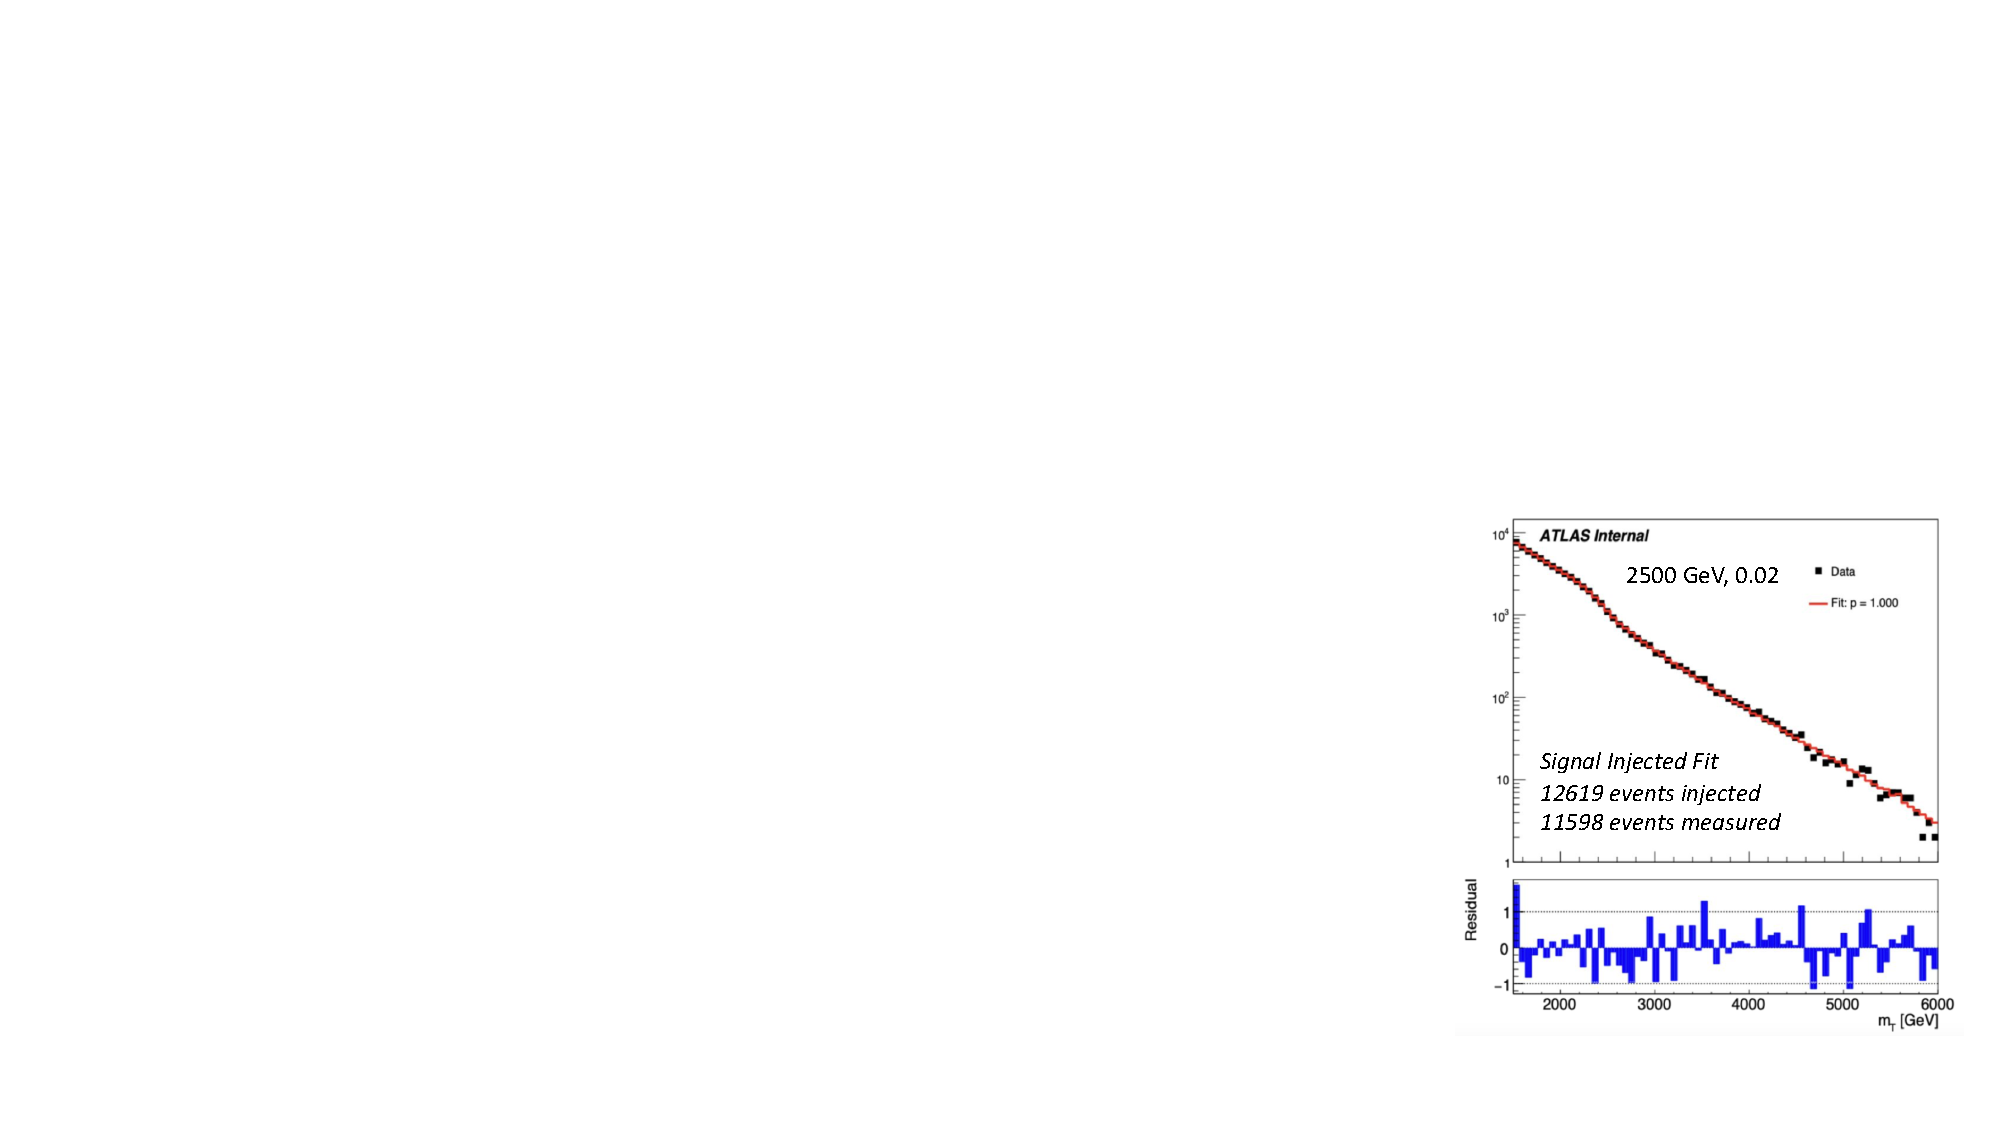
\includegraphics[width=0.6\textwidth]{figures/stats/splusb_sigInj}
    \caption{Example S+B fits on a background \mt~spectrum with injected signal from the point (2500 GeV, \rinv=0.2).
    \label{fig:splusb_sigInj}}
\end{figure}

\paragraph{Signal Injection in Asimov Data}
To better understand the correlations of fit errors in the above single-template injection test and avoid drawing conclusions from a single scenario, signal injection tests using Asimov data will be performed before unblinding. 
50 Asimov trials are run for representative signal points across Z' mass and \rinv.

%Bias within the Asimov signal injection test could indicate a lack of sufficient normalization uncertainties on the signal model. 
%In the event of systematic mismeasurement in signal injection, the spurious signal uncertainty as derived from Loose-not-tight or additional uncertainties will be considered.

Figure~\ref{fig:siginj_asimov} provides the results of these tests. 
The uncertainty of the measurement varies according to mass point, due to the larger relative background for lower mass points. 
However, a strong linear relationship between amount of signal injected and amount of signal measured is observed for all signal points, which is the key feature.
\begin{figure}[!htbp]
\centering
   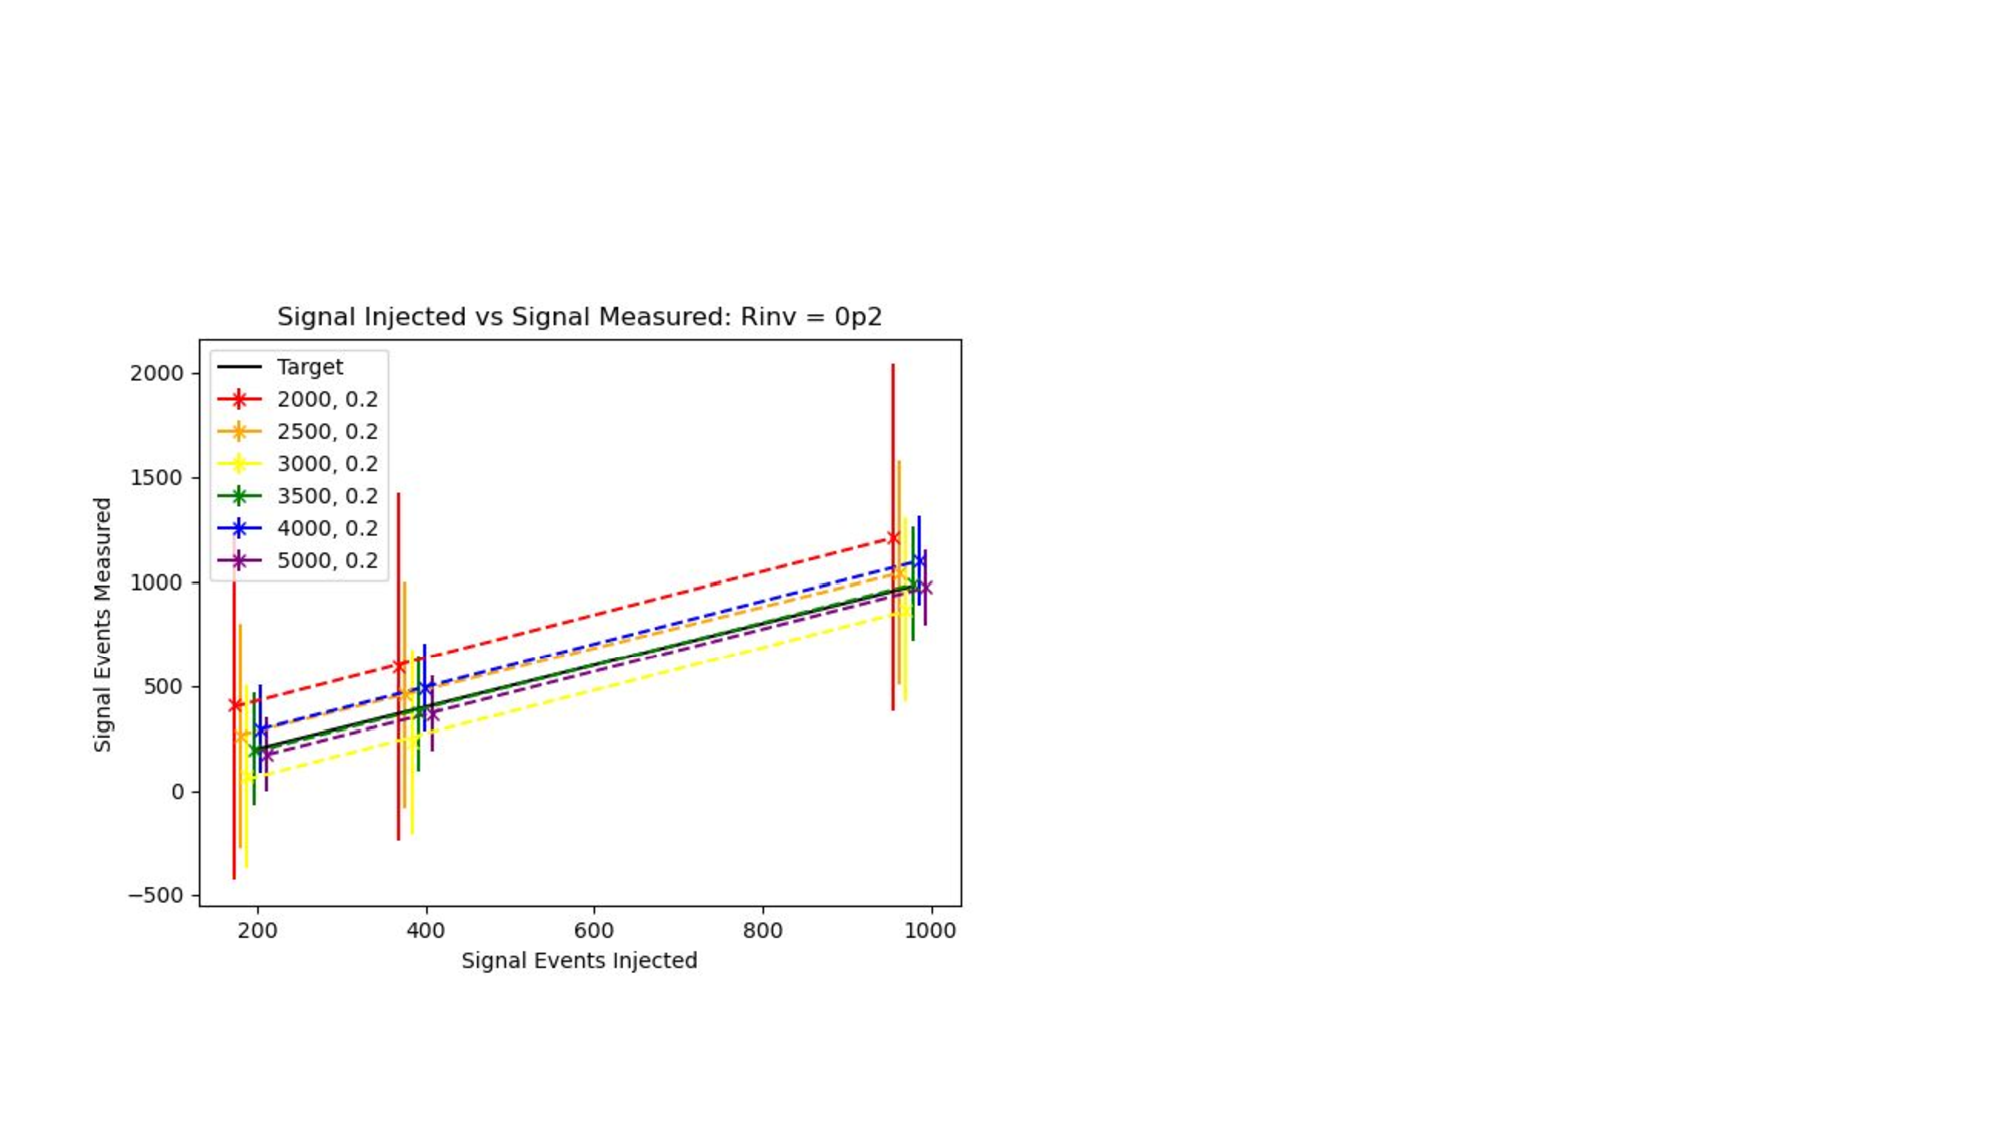
\includegraphics[width=0.45\textwidth]{figures/stats/siginj_asimov_02}
   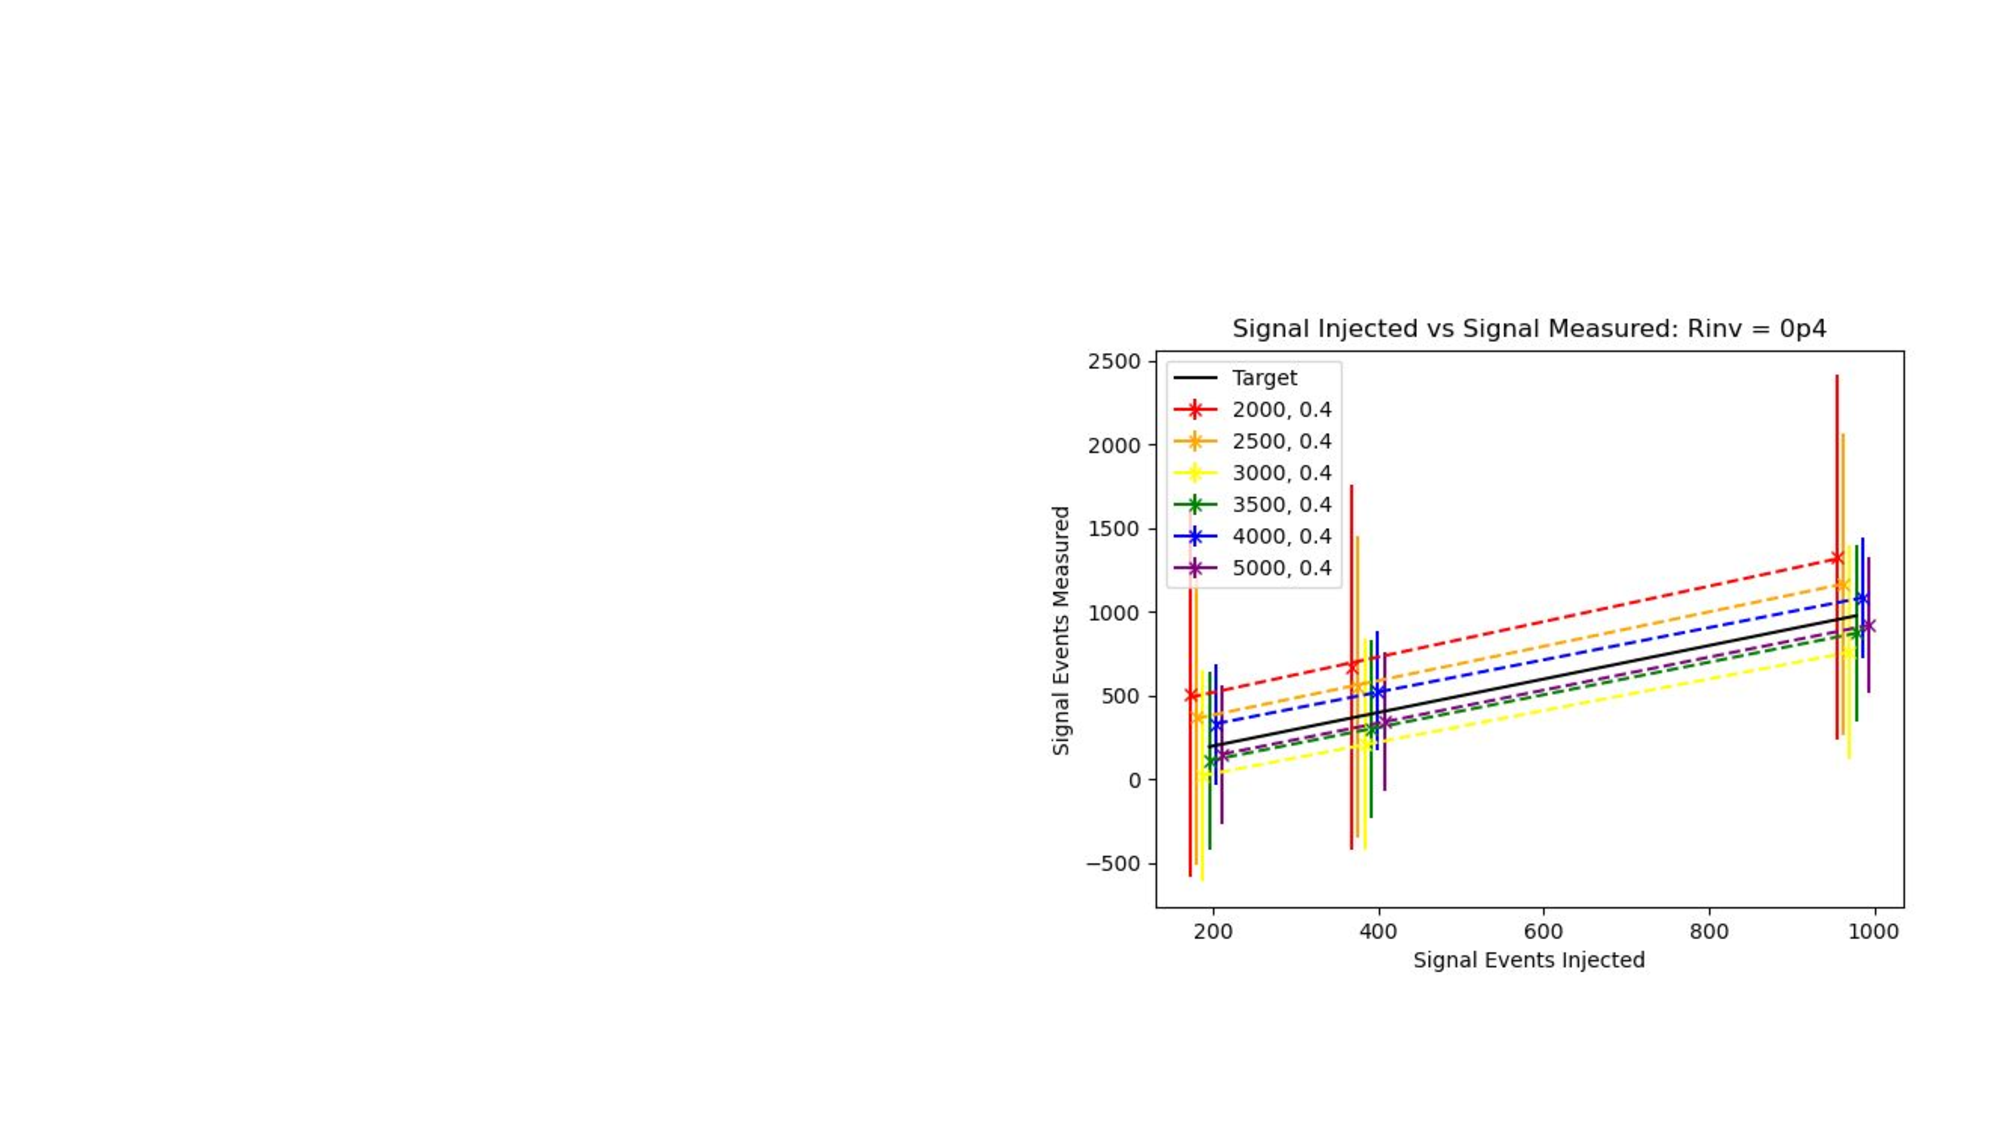
\includegraphics[width=0.45\textwidth]{figures/stats/siginj_asimov_04}
   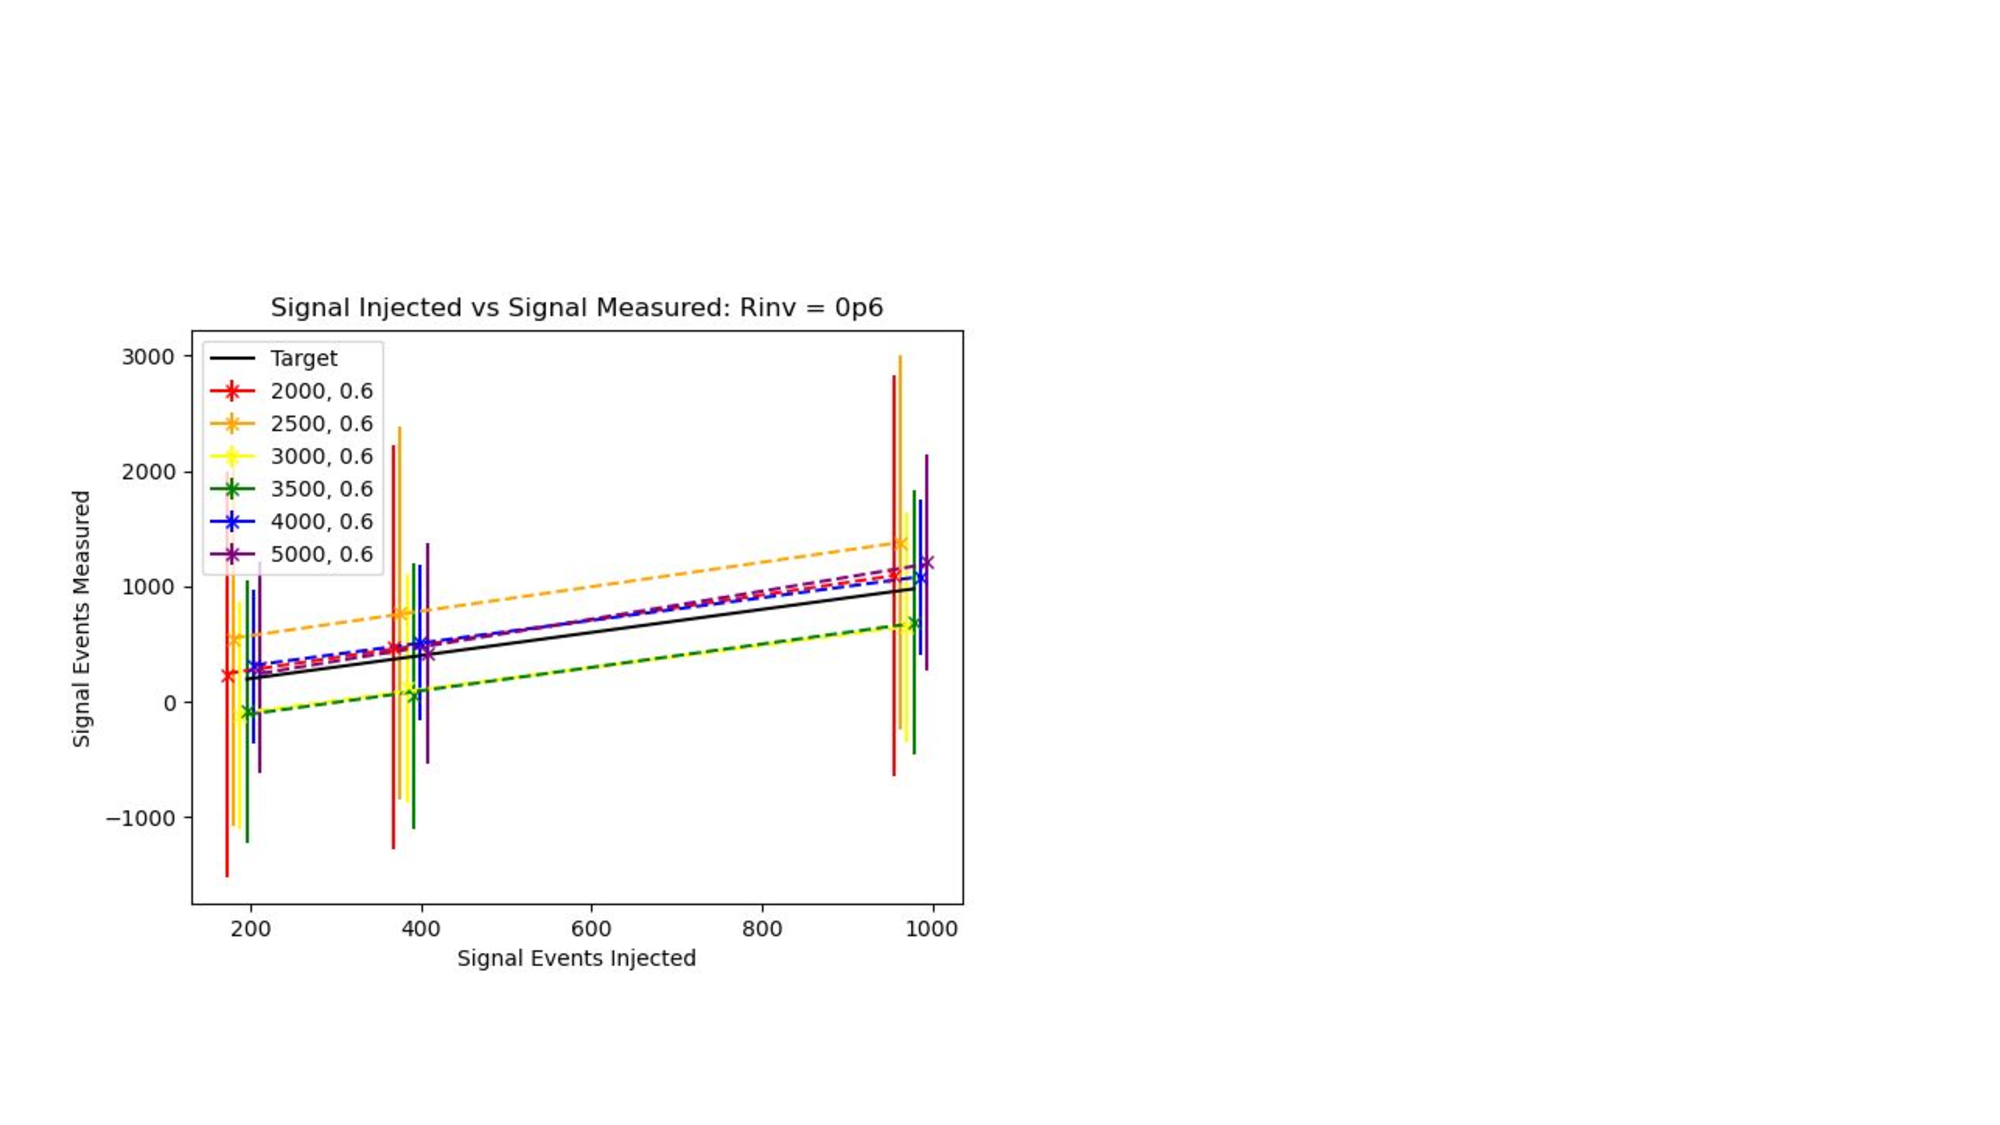
\includegraphics[width=0.45\textwidth]{figures/stats/siginj_asimov_06}
   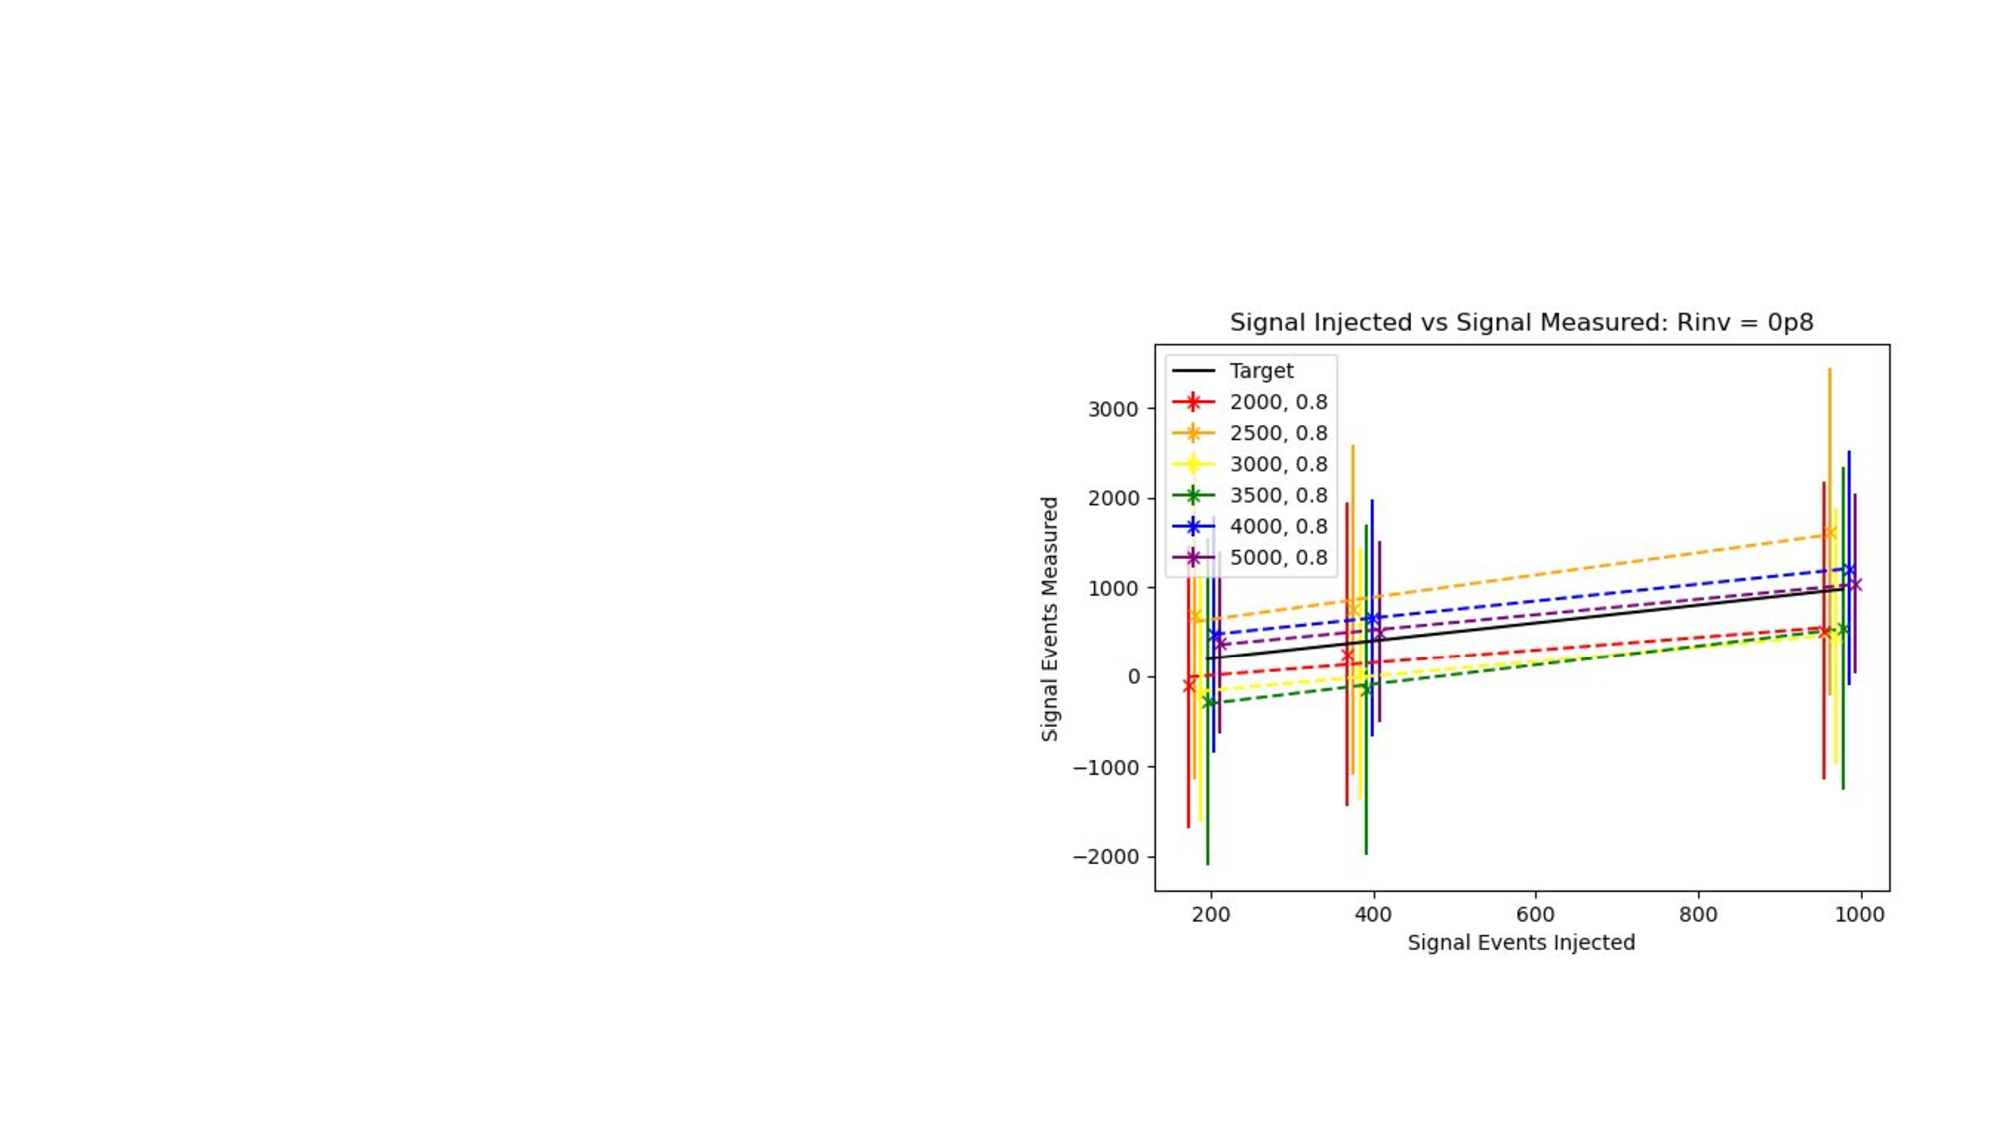
\includegraphics[width=0.45\textwidth]{figures/stats/siginj_asimov_08}
   \caption{Measured signal at a variety of injected values (1x, 2x, and 5x$\sqrt{b}$), for all signal points in the grid, \rinv=0.2 (top left), 0.4 (top right), 0.6 (bottom left), and 0.8 (bottom right).
%he requirement relative to $\sigma_{\text{fit}}$ is met for every signal point and injected signal size, thus satisfying the OR criteria from Equation~\ref{eq:spursig}.
    \label{fig:siginj_asimov}}
\end{figure}

%------------------------------------------------- 
\subsubsection{Expected Sensitivity}
\label{subsec:fit_expsens}

Limits are obtained by determining the cross section of the signal that can be excluded to 95\% confidence. 
Figure~\ref{fig:limits_exp_1D} shows the expected limits obtained from S+B fits to statistically identical \mt~spectra from the CR region (which is closest in \mt~shape to the SR according to MC studies). 
%Figure~\ref{fig:limits_exp_1D_asimov} shows the expected limits obtained from an average of 50 Asimov toys thrown from the CR.
%The limits are very stable across individual data fits and Asimov, as well as across the CR and VR.
%The alignment of fluctuations between the single CR fit and Asimov toys indicates that the particular shape of data in the CR influences the shape of the limits.
%The limits shown come from an average of 10 Asimov pseudodata fits of the CR. Figure~\ref{fig:perc_success_limit} shows the percentage of Asimov limit tests that result in a successful fit. 

Considerable exclusion power is predicted for low \rinv~signal points, with the higher \rinv~points presenting more difficulty due to the very broad signal bump. 
A similar trend is observed in the CMS s-channel search~\cite{cms_schan}.

\begin{figure}[!htbp]
\centering
   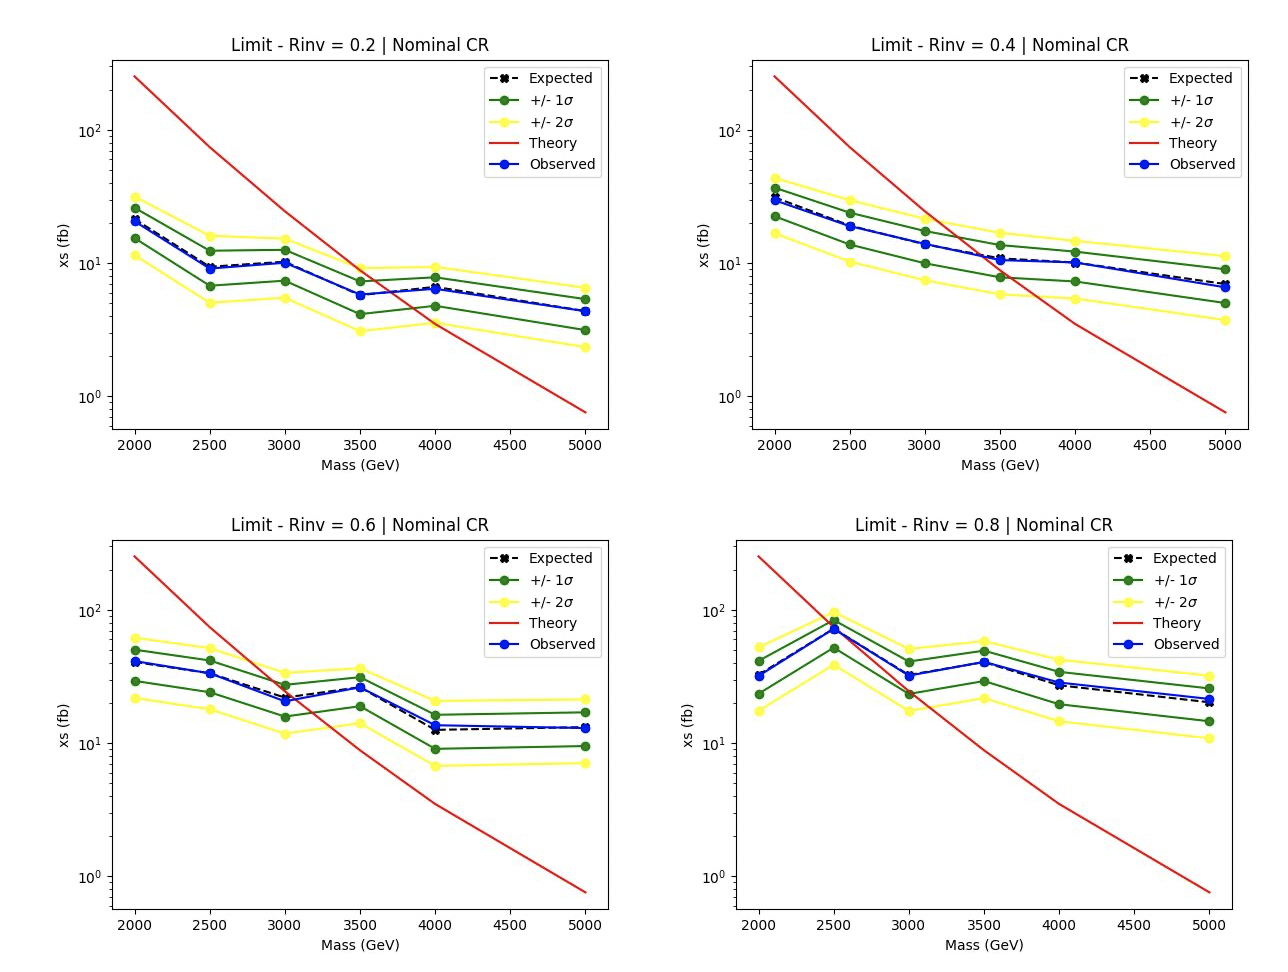
\includegraphics[width=0.95\textwidth]{figures/stats/limits_exp_1D}
    \caption{95\% C.L. upper limits for signal models across Z' mass, for four different \rinv~fractions, from the CR region (without systematics).
    \label{fig:limits_exp_1D}}
\end{figure}
%\begin{figure}[!htbp]
%\centering
%   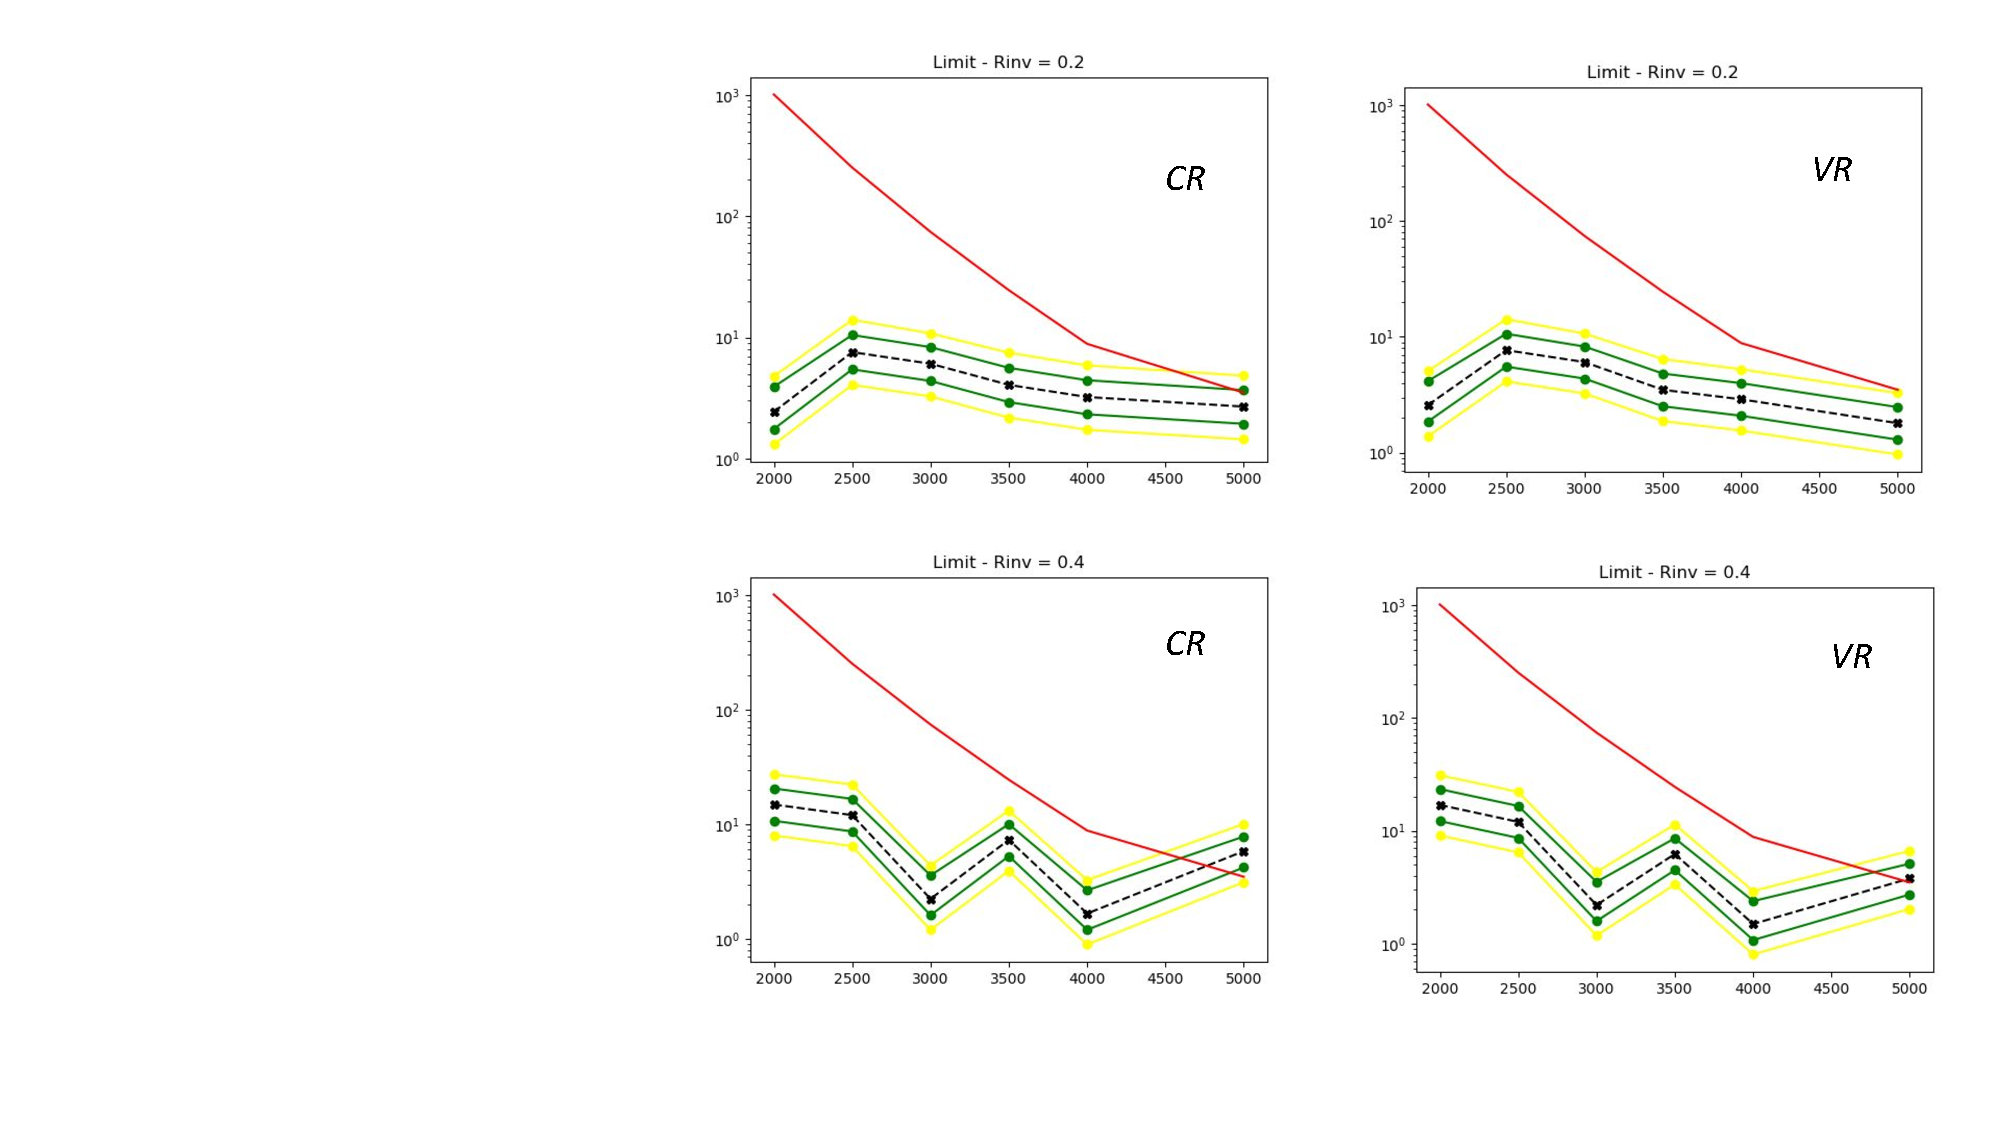
\includegraphics[width=0.9\textwidth]{figures/stats/limits_exp_1D_asimov_1}
%   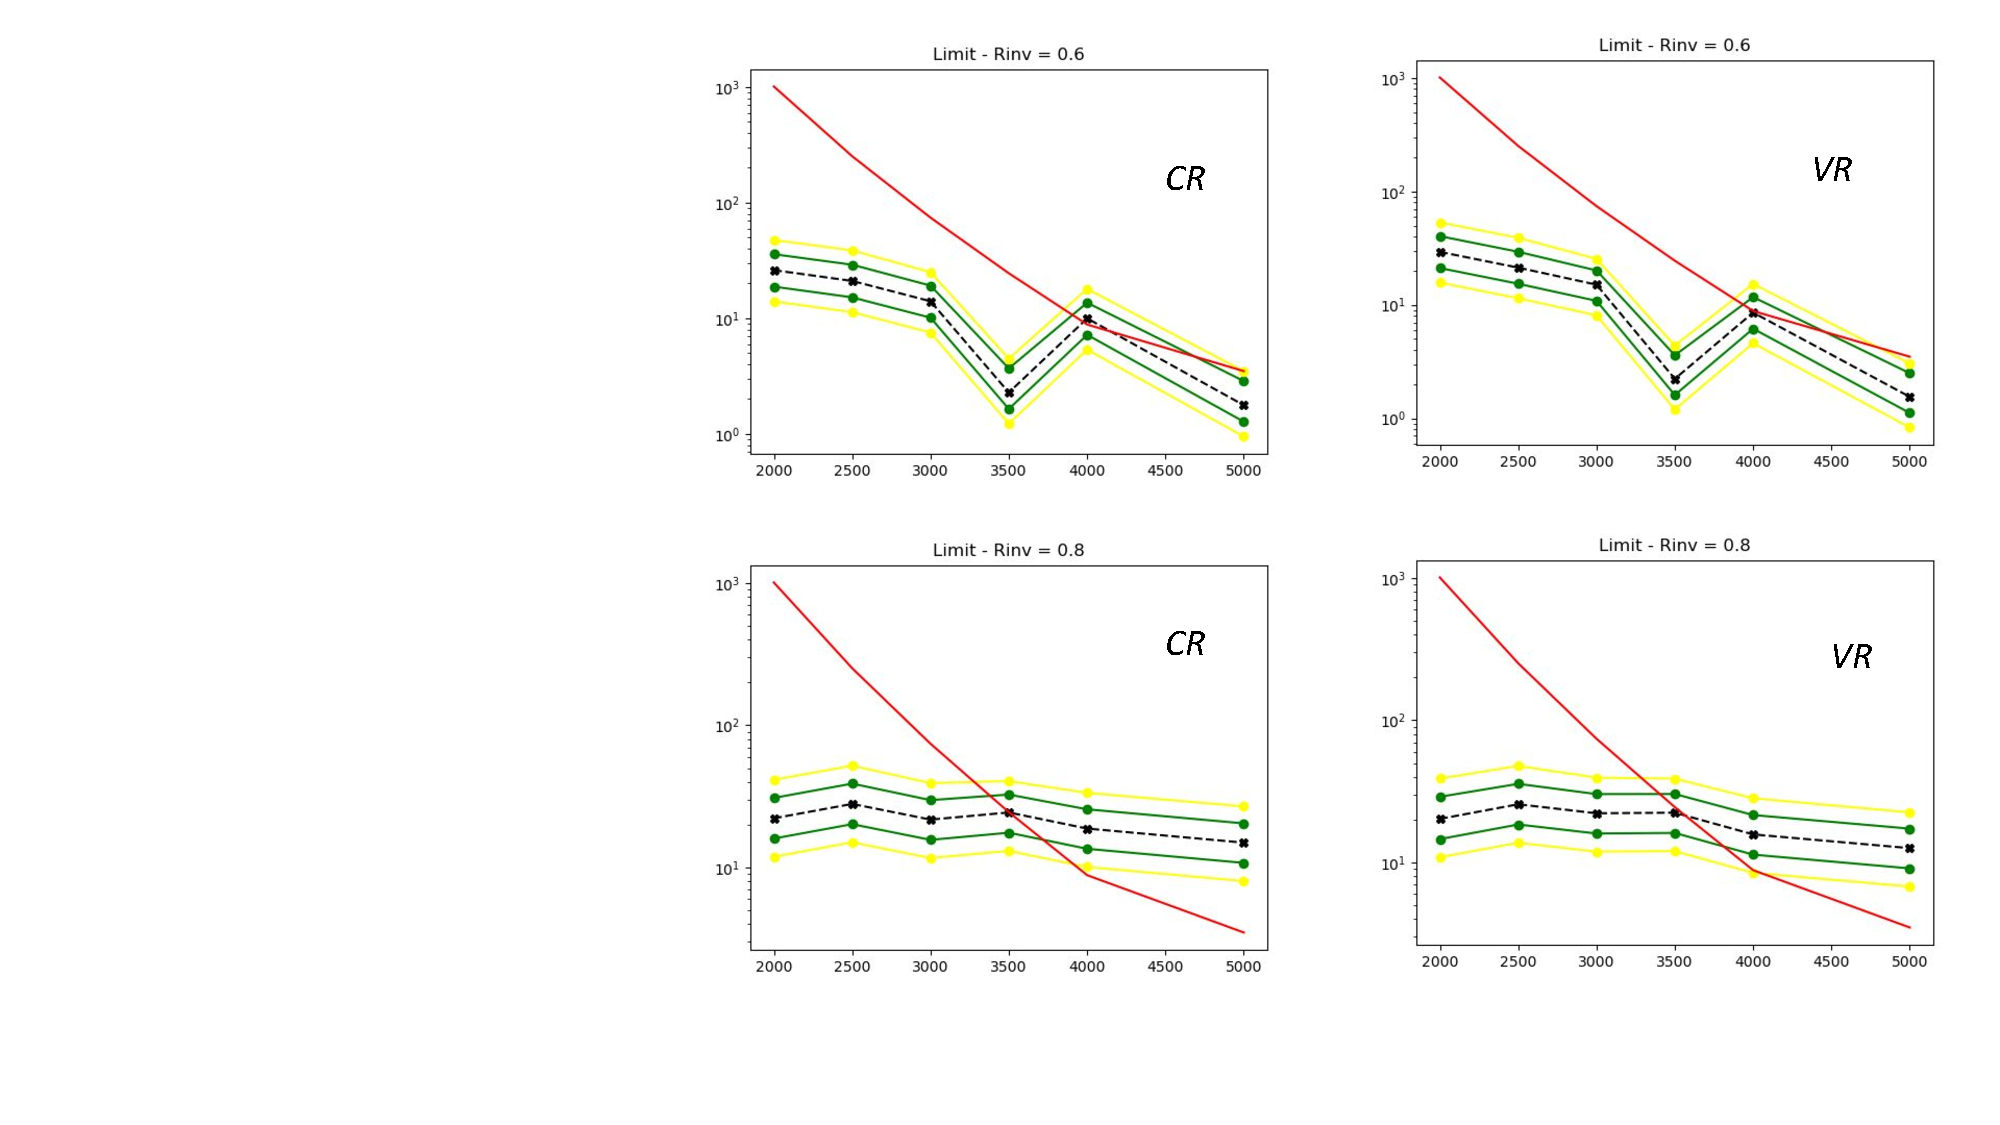
\includegraphics[width=0.9\textwidth]{figures/stats/limits_exp_1D_asimov_2}
%    \caption{95\% C.L. upper limits for signal models across Z' mass, for four different \rinv~fractions, using an average of 50 Asimov pseudo-data tests from the CR (left) and VR (right) (without systematics).
%    \label{fig:limits_exp_1D_asimov}}
%\end{figure}

%\begin{figure}[!htbp]
%\centering
%   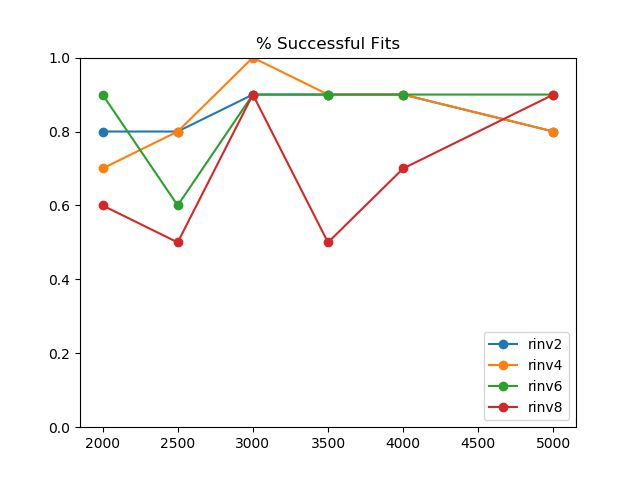
\includegraphics[width=0.6\textwidth]{figures/stats/perc_success_limit}
%    \caption{Percent of Asimov pseudodata S+B fits with successful fit and successful limit convergence.
%    \label{fig:perc_success_limit}}
%\end{figure}

A 2D limit presentation is also being considered, in the (\rinv, mass) plane.


\clearpage



%------------------------------------------------- 
\subsection{Discovery Strategy}
\label{subsec:fit_bh}

Model-independent fits for the discovery region are performed using \textsc{pyBumpHunter} \cite{bumphunt}.
The strategy consists of comparing the data in a given \mt~spectrum of interest to a background estimation derived by performing the polynomial fit and sampling from the post-fit function into a histogram.

The polynomial fit is done to an \mt~distribution with 180 bins (25 GeV wide), half the width of the fits in the SVJ Fit region (50 GeV wide). %90 bins, as with the PFN 
The narrower bins allow for rebinning based on the \textit{signal mass resolution} of the SVJ signals.
The binning strategy is outlined in Appendix~\ref{app:binning}.

Figure~\ref{fig:bkgfit_data_crvr_antelope} shows the fit and residuals with of the polynomial with the narrower binning in the CR and the Discovery VR data.
Figure~\ref{fig:postfit_param_antelope} shows the post-fit values of the fit parameters and their uncertainties for the CR and VR. 
These results indicate good ability of the 5-parameter polynomial to model the ANTELOPE selected data.

\begin{figure}[!htbp]
\centering
   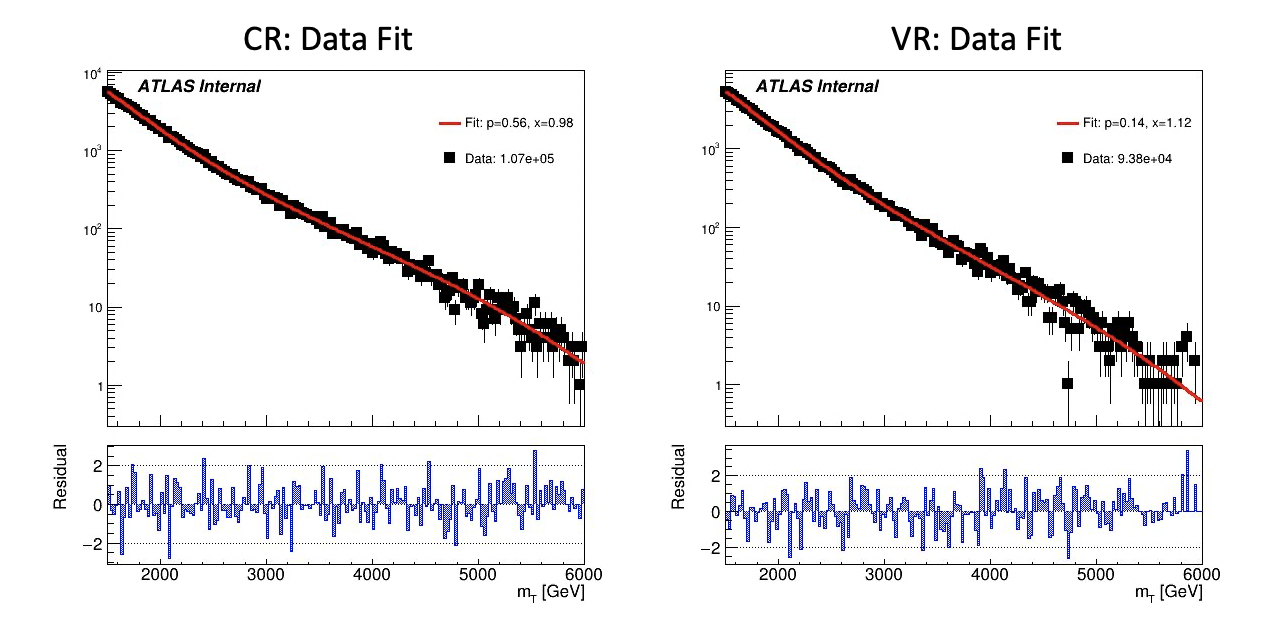
\includegraphics[width=0.95\textwidth]{figures/stats/bkgfit_data_crvr_antelope}
    \caption{Post-fit function and residuals for the ANTELOPE CR and VR.
    \label{fig:bkgfit_data_crvr_antelope}}
\end{figure}

\begin{figure}[!htbp]
\centering
   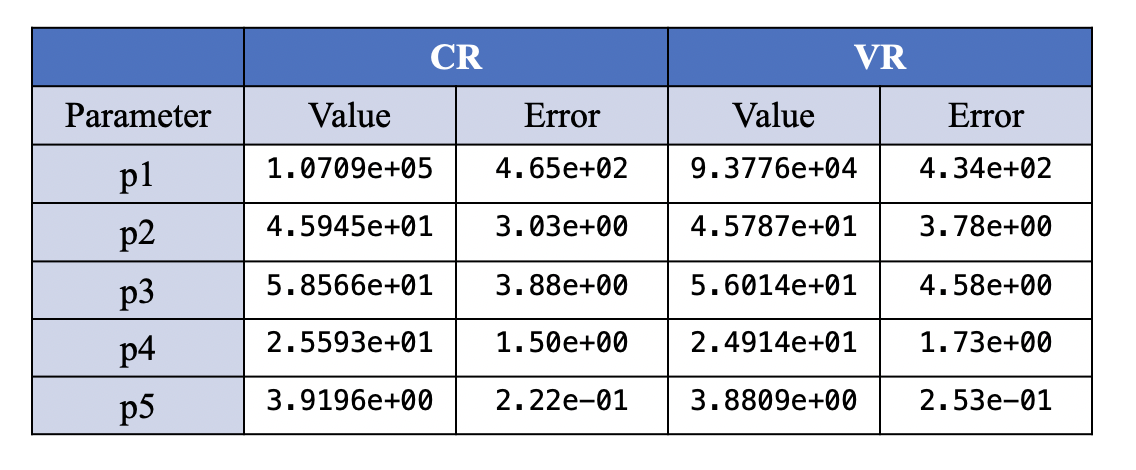
\includegraphics[width=0.65\textwidth]{figures/stats/postfit_param_antelope}
    \caption{Post-fit parameters for the ANTELOPE CR and VR.
    \label{fig:postfit_param_antelope}}
\end{figure}

The studies shown in Section~\ref{subsec:fit_bkgonly} validate the robustness of the background polynomial fit. 
The narrower bins are the only difference for polynomial fitting between the SVJ Fit and Discovery Fit strategies, and they are not observed to reduce the quality or consistency of the fit. 

%----------------------------------------------------------------------------------------
\subsubsection{BumpHunter Fits}
\label{subsec:bhfits}

The signal mass resolution binning strategy described in Appendix~\ref{app:binning} creates a monotonically increasing set of bins. 
While the SVJ signals help inform the binning, the binning is still broadly applicable to a variety of potential signal models.
The mass resolution of any resonant signal generally widens as the mass of the mediator particle increases.
A similar strategy and binning was used in the generic heavy resonance search presented in Ref.~\cite{yxh}.
The resulting set of 15 bins to be used in the BumpHunter fits varies in width from 100 GeV at the \mt~core to 925 GV in the \mt~tail. 

Figure~\ref{fig:antelope_bh_crvr} shows the result of running BumpHunter over the rebinned CR and VR \mt~spectra.
The background estimation is given by polynomial fit function. 
The high p-values (>0.01) indicate good agreement with the background estimation.
\begin{figure}[!htbp]
\centering
   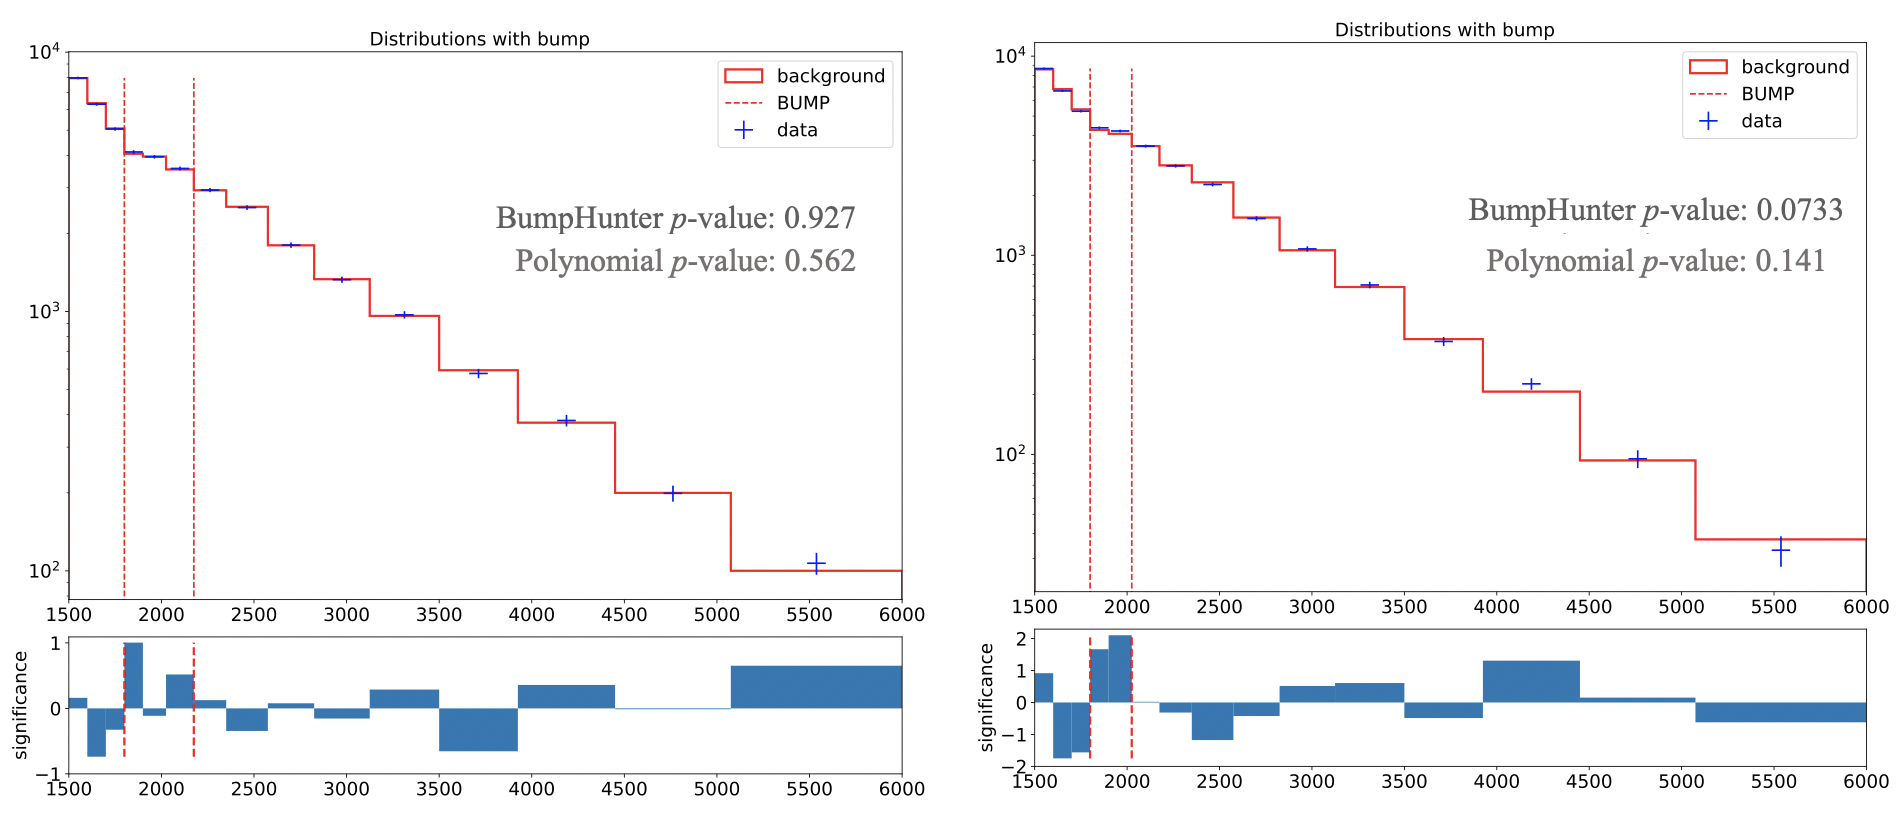
\includegraphics[width=0.95\textwidth]{figures/stats/antelope_bh_crvr}
    \caption{BumpHunter fits on the ANTELOPE \mt~spectra for both the CR (left) and VR (right). In a signal-depleted region, good agreement with the background estimation is observed.
    \label{fig:antelope_bh_crvr}}
\end{figure}

Figure~\ref{fig:bh_asimov_pvals} shows BumpHunter p-values over 100 Asimov trials, where each toy is scaled to the statistics of the SR.
The agreement is generally very good, as the p-values trend towards higher values.
No fits with a \textit{spurious signal} are found.
A spurious signal would be indicated by a fit with a p-value $<$ 0.01, indicting a bump of at least $2\sigma$ significance.
\begin{figure}[!htbp]
\centering
   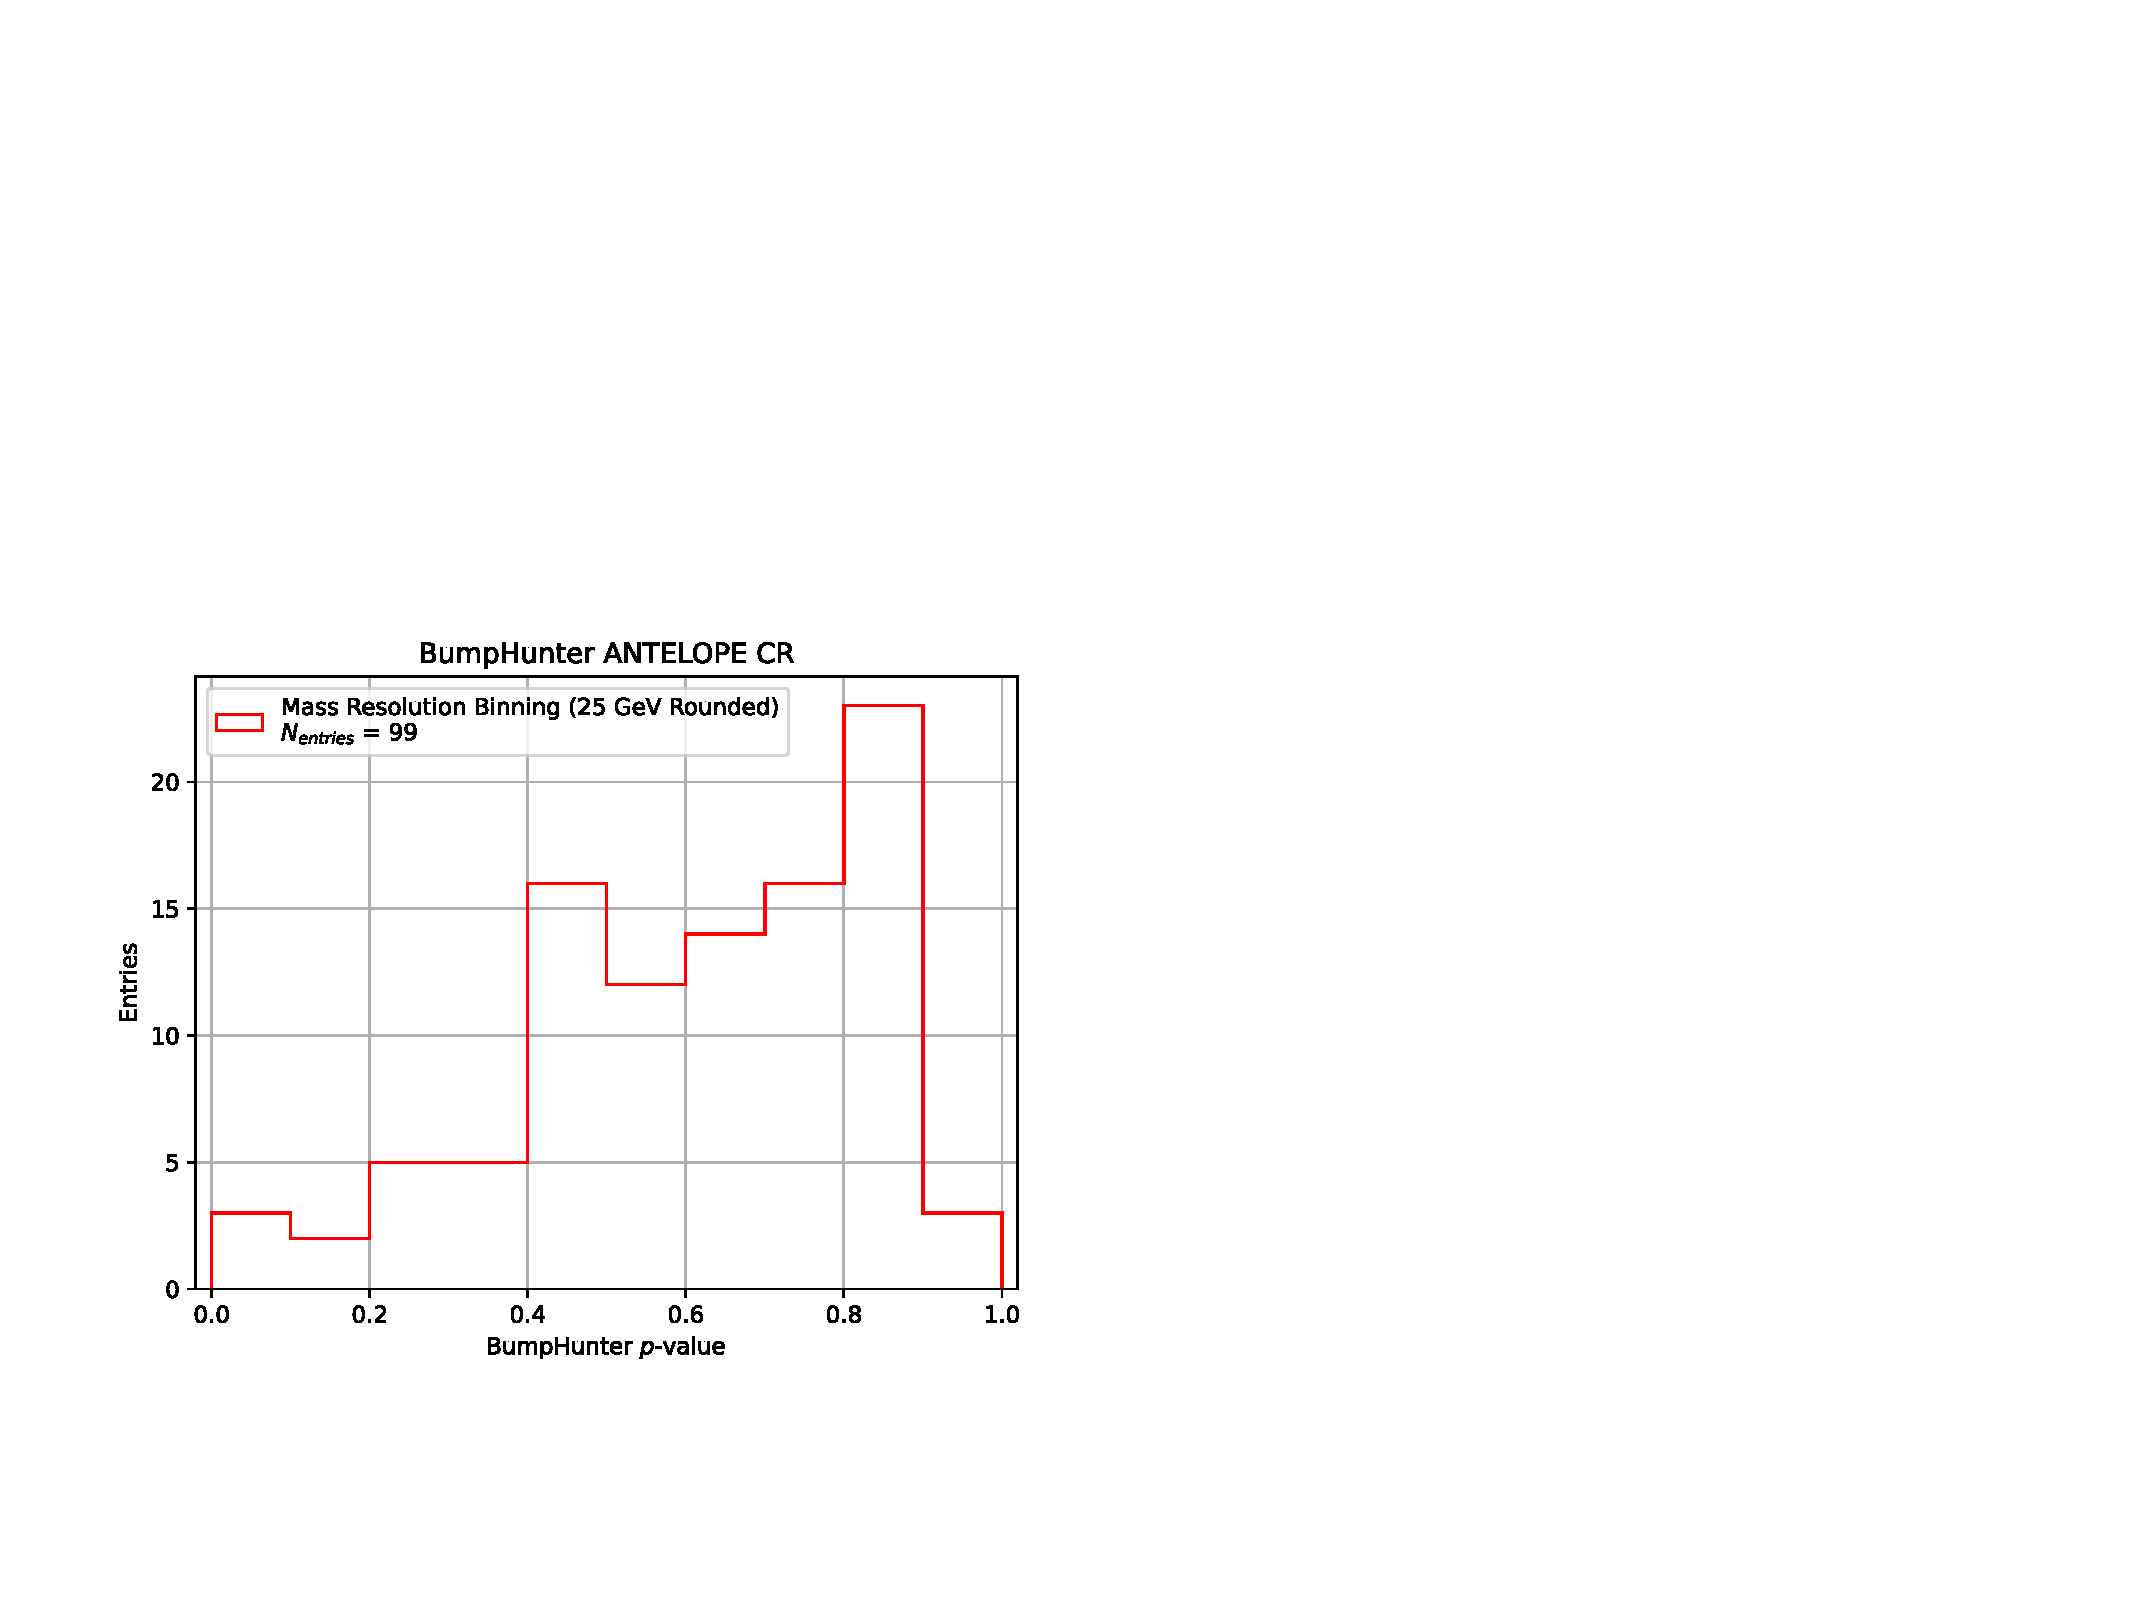
\includegraphics[width=0.45\textwidth]{figures/stats/bh_asimov_pvals_cr}
   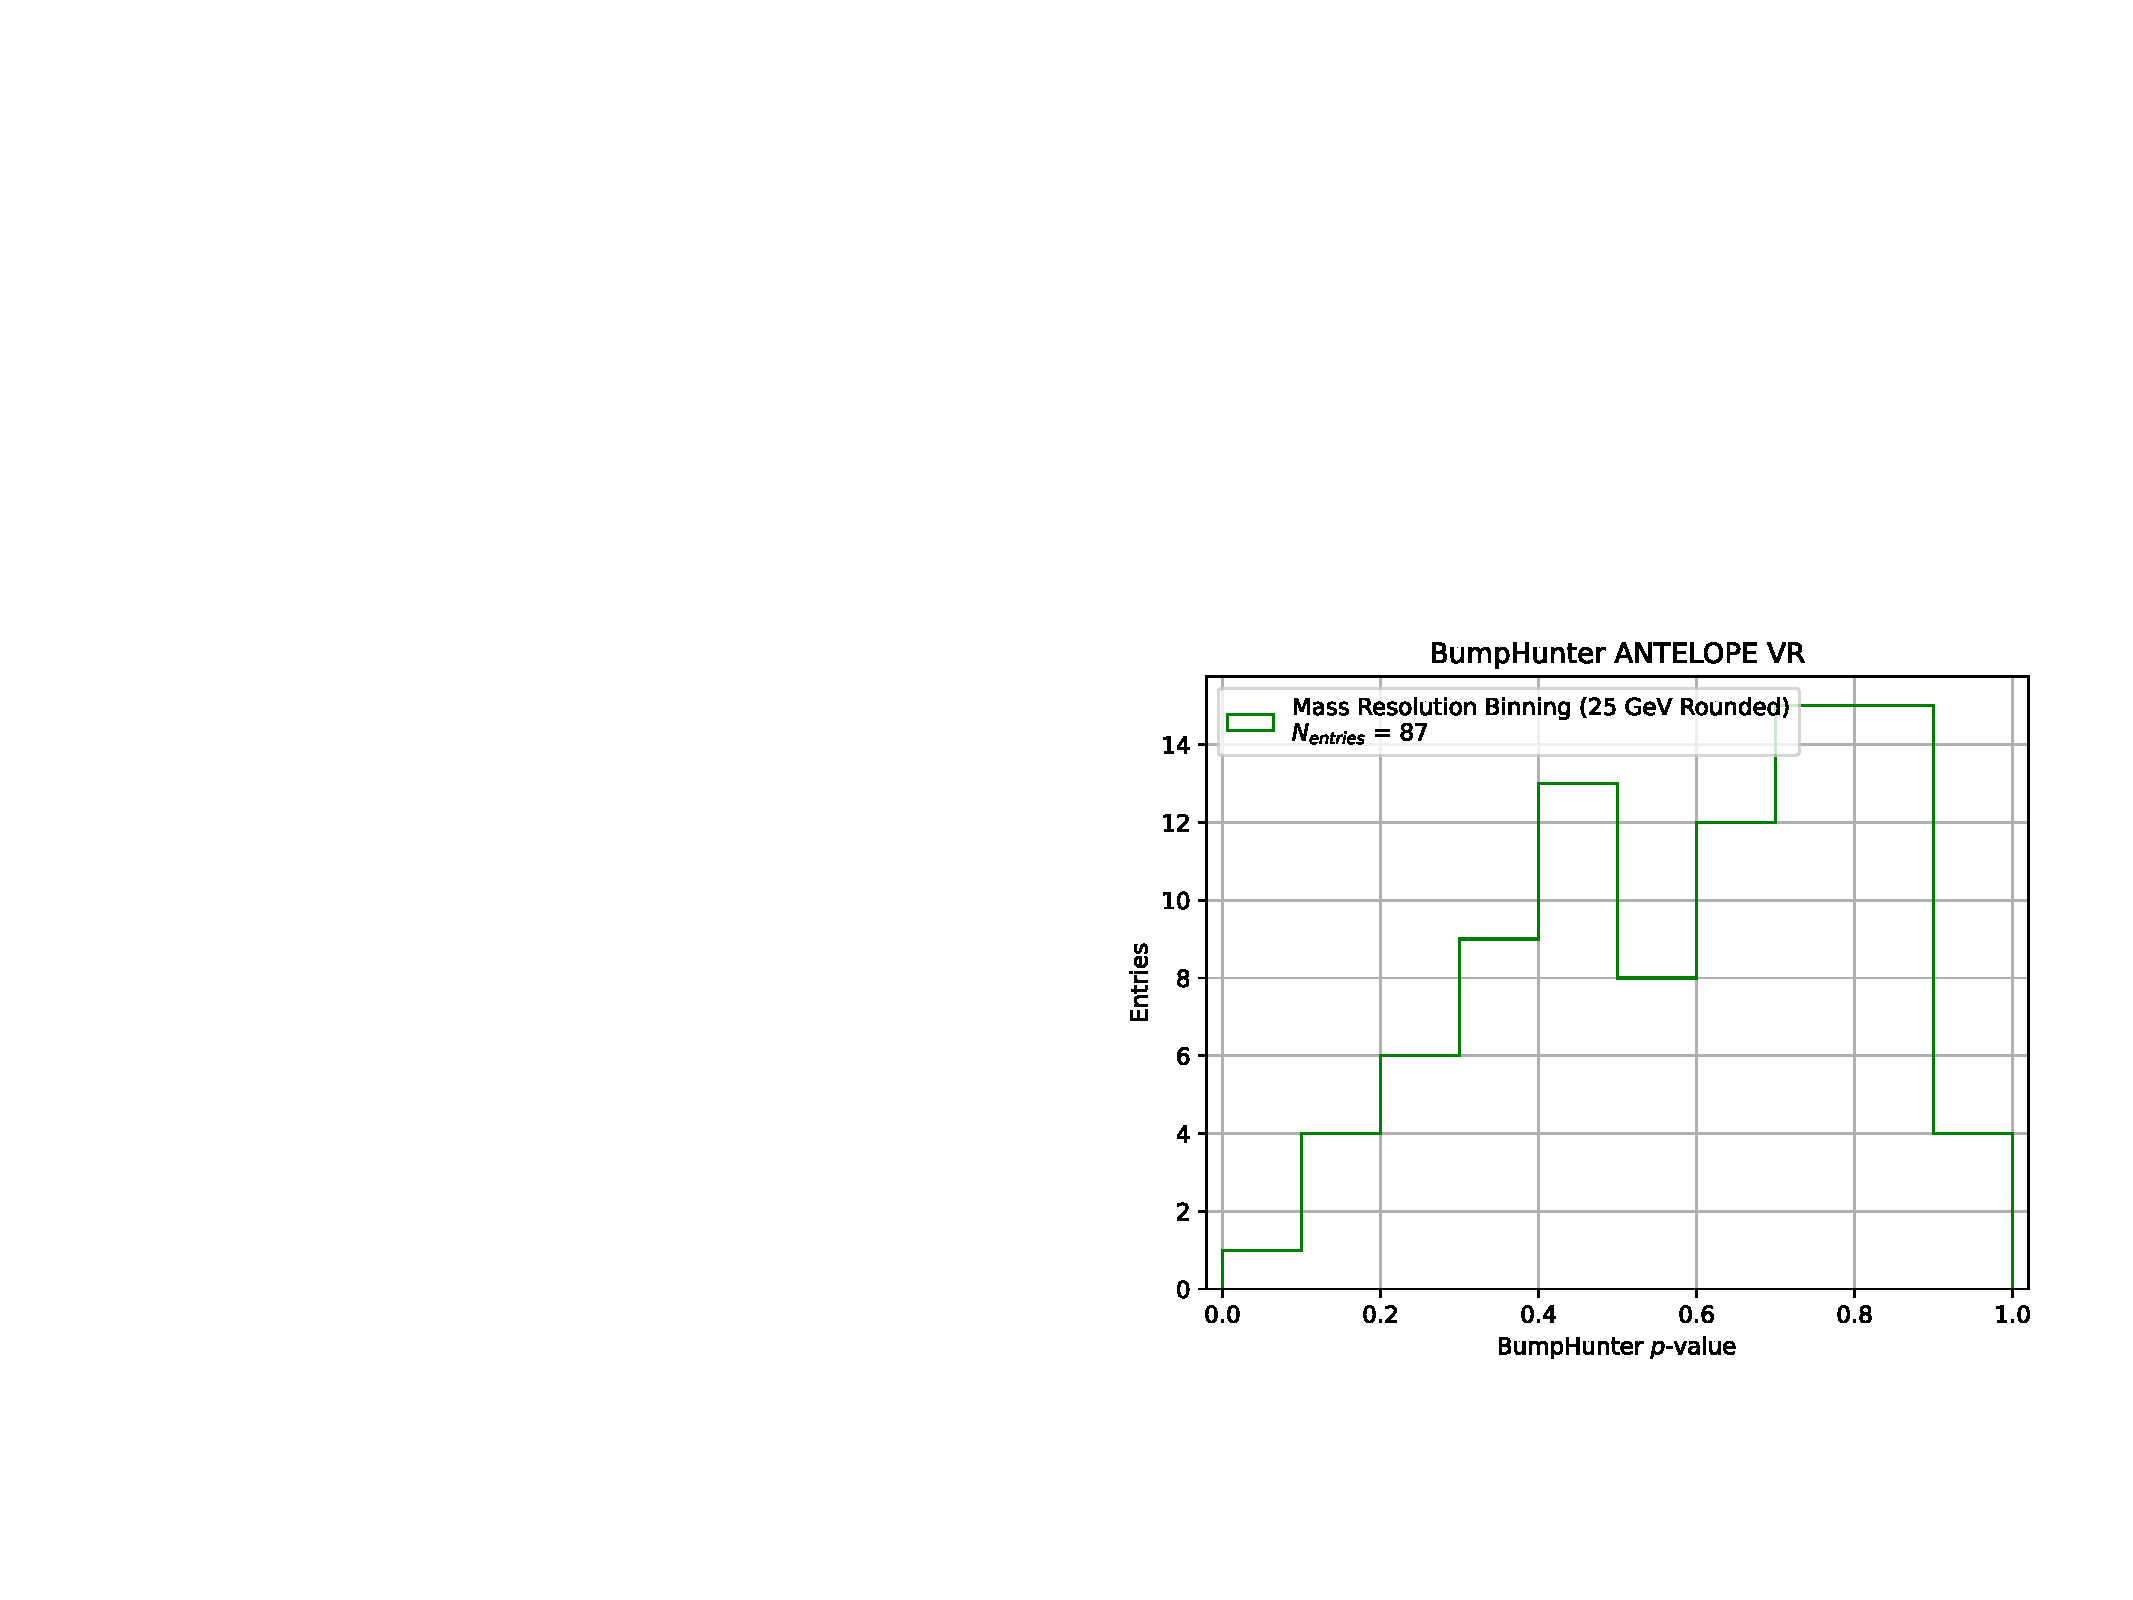
\includegraphics[width=0.45\textwidth]{figures/stats/bh_asimov_pvals_vr}
    \caption{BumpHunter p-values extracted for 100 Asimov toys for both the ANTELOPE CR (left) and VR (right).
    \label{fig:bh_asimov_pvals}}
\end{figure}

%----------------------------------------------------------------------------------------
\subsubsection{BumpHunter Signal Injection}
\label{subsec:bhsiginj}

To explore a model independent signal hypothesis, signal injection tests in the ANTELOPE region are done with generic Gaussian shapes.
Two Gaussian models are built with a mean ranging from 2000 GeV to 5000 GeV and a standard deviation equal to 10 or 20\% the mean value.
Figure~\ref{fig:gauss_inj} illustrates an injected Gaussian and its effect on the \mt~distribution.
The 20\% gaussian represents the widest possible signals we might be sensitive to with a BH strategy, while the 10\% injection represents a narrower signal peak. 

\begin{figure}[!htbp]
\centering
   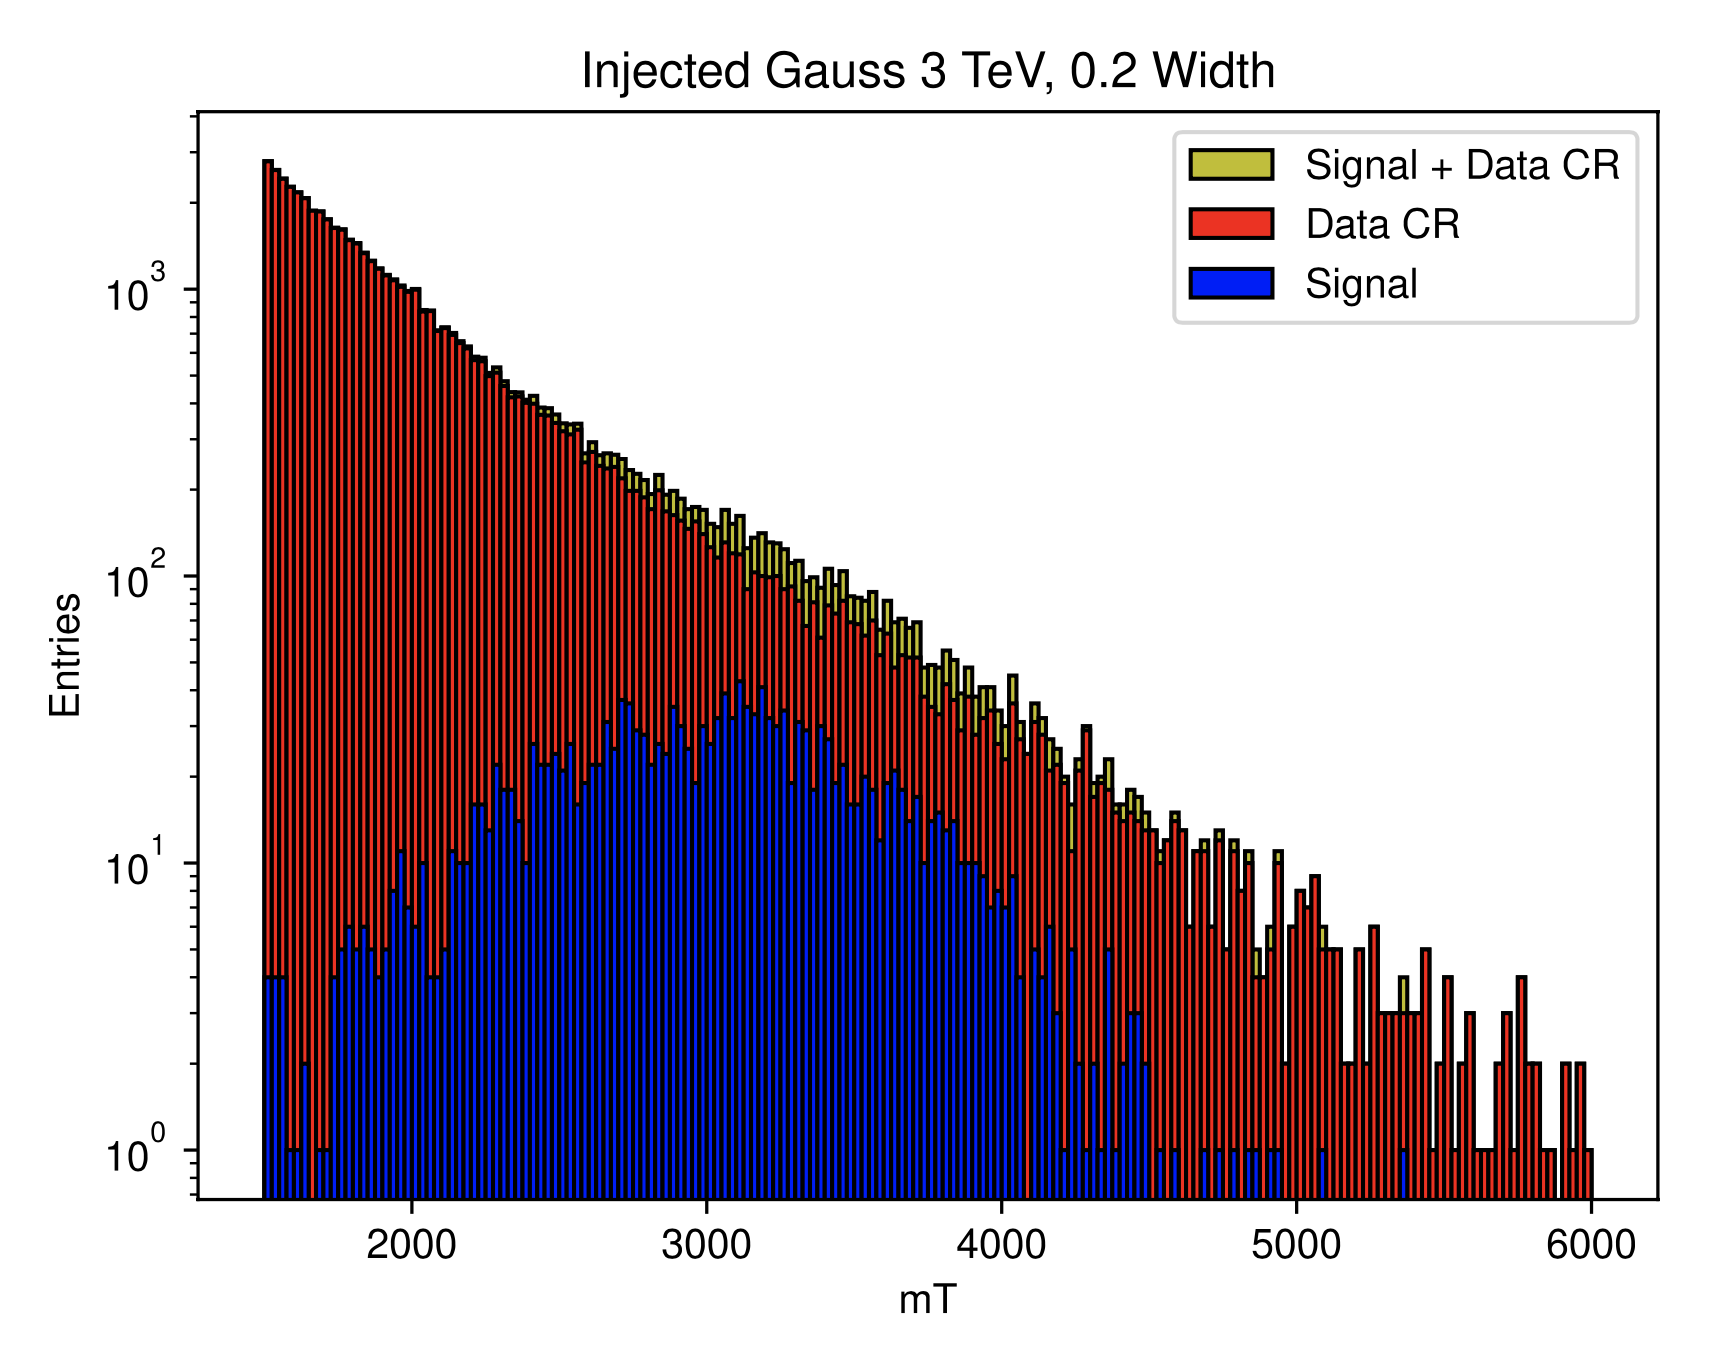
\includegraphics[width=0.5\textwidth]{figures/stats/gauss_inj}
    \caption{Example injected gaussian signal.
    \label{fig:gauss_inj}}
\end{figure}

%The polynomial fit framework is run over background-only Asimov data to determine the injection level, as discussed in Section~\ref{subsec:fit_expsens}. 
%It should be noted that the $5\sigma$ injection level as determined by the polynomial fit is an underestimate, as the flexibility of the fit absorbs some of the signal.

An estimated $5\sigma$ of signal is injected for these tests.
The estimate is derived from the polynomial fitting framework, and is therefore an underestimate, as the flexibility of the polynomial fit absorbs some of the signal.
Therefore we do not expect to measure $5\sigma$ significance with the BH approach, but rather hope to see that some level of signal (at least $\geq2\sigma$ significance)  is observed by the BumpHunter framework. 

Results are obtained by averaging over 100 toys for each injection.
Figure~\ref{fig:siginj_bh} shows the resulting max local significance (in an \mt~bin) and the location of the determined bump, indicating a good response of the BumpHunter framework for detecting generic \mt~resonances at the right location.
Only the 5000 GeV 20\% width point is not properly identified by the framework. 
While some sensitivity is lost due to the flexible nature of the fitting framework, the ability to identify a bump with substantial local significance in the correct location is observed.
Figure~\ref{fig:bh_bump_example} shows an example of the identified bump.

\begin{figure}[!htbp]
\centering
   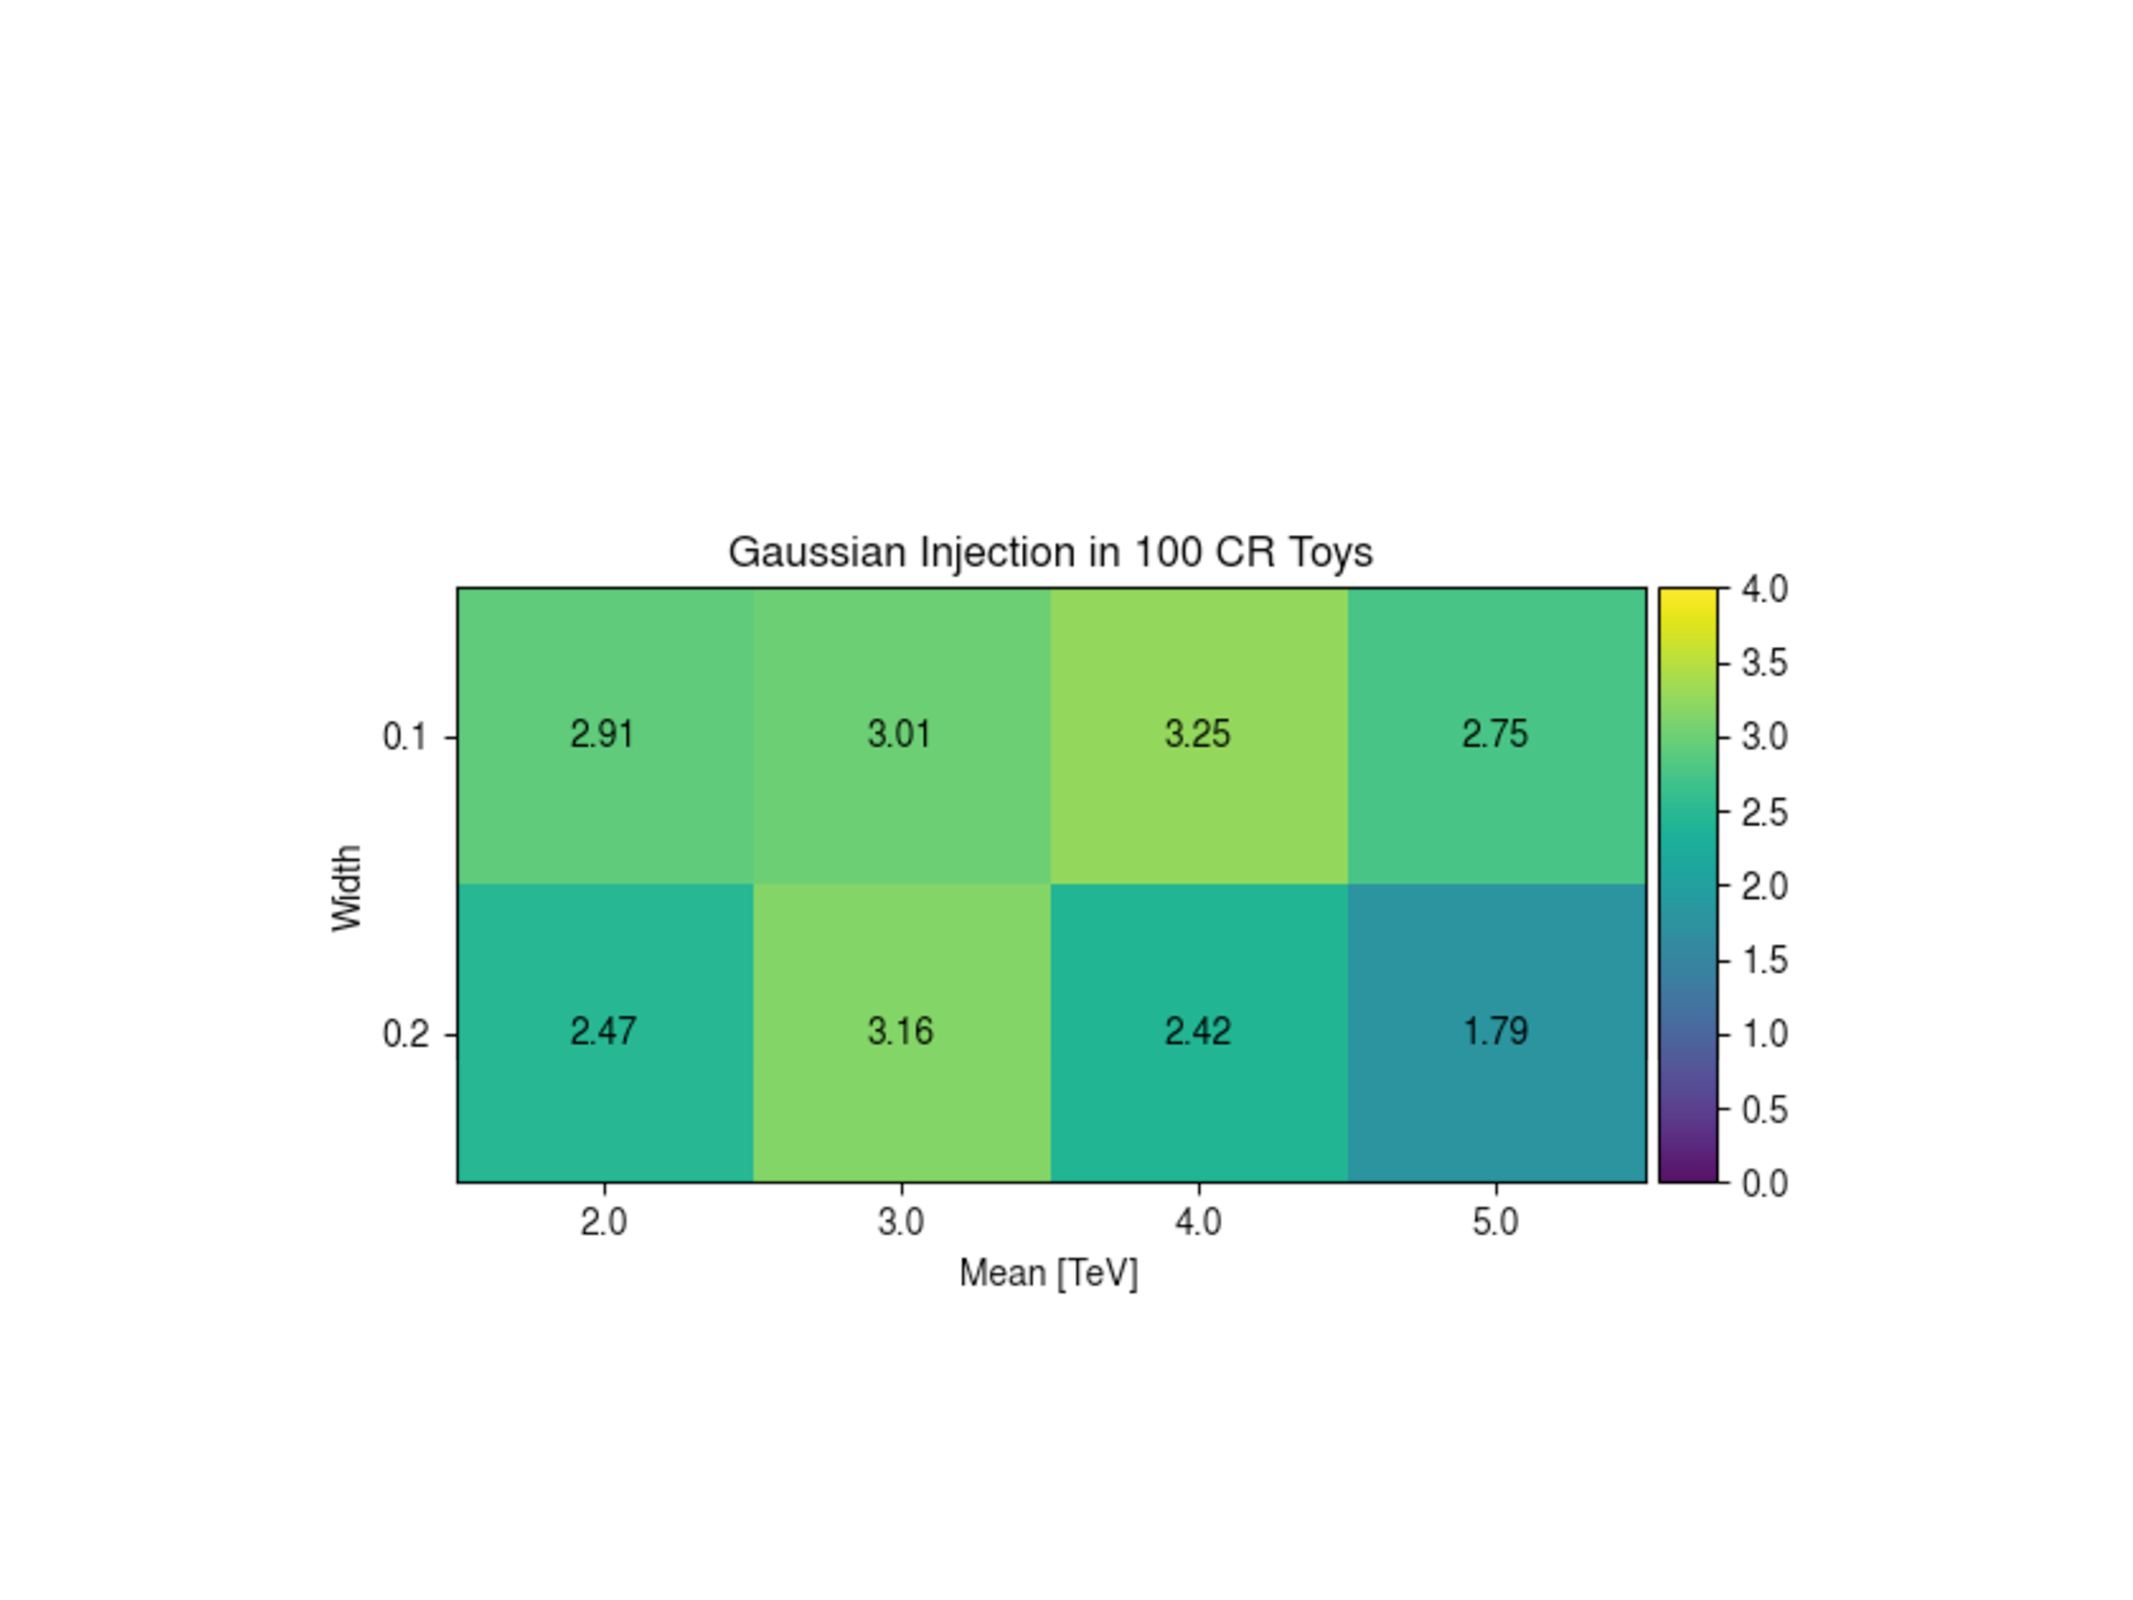
\includegraphics[width=0.65\textwidth]{figures/stats/siginj_bh_localsig.pdf}
   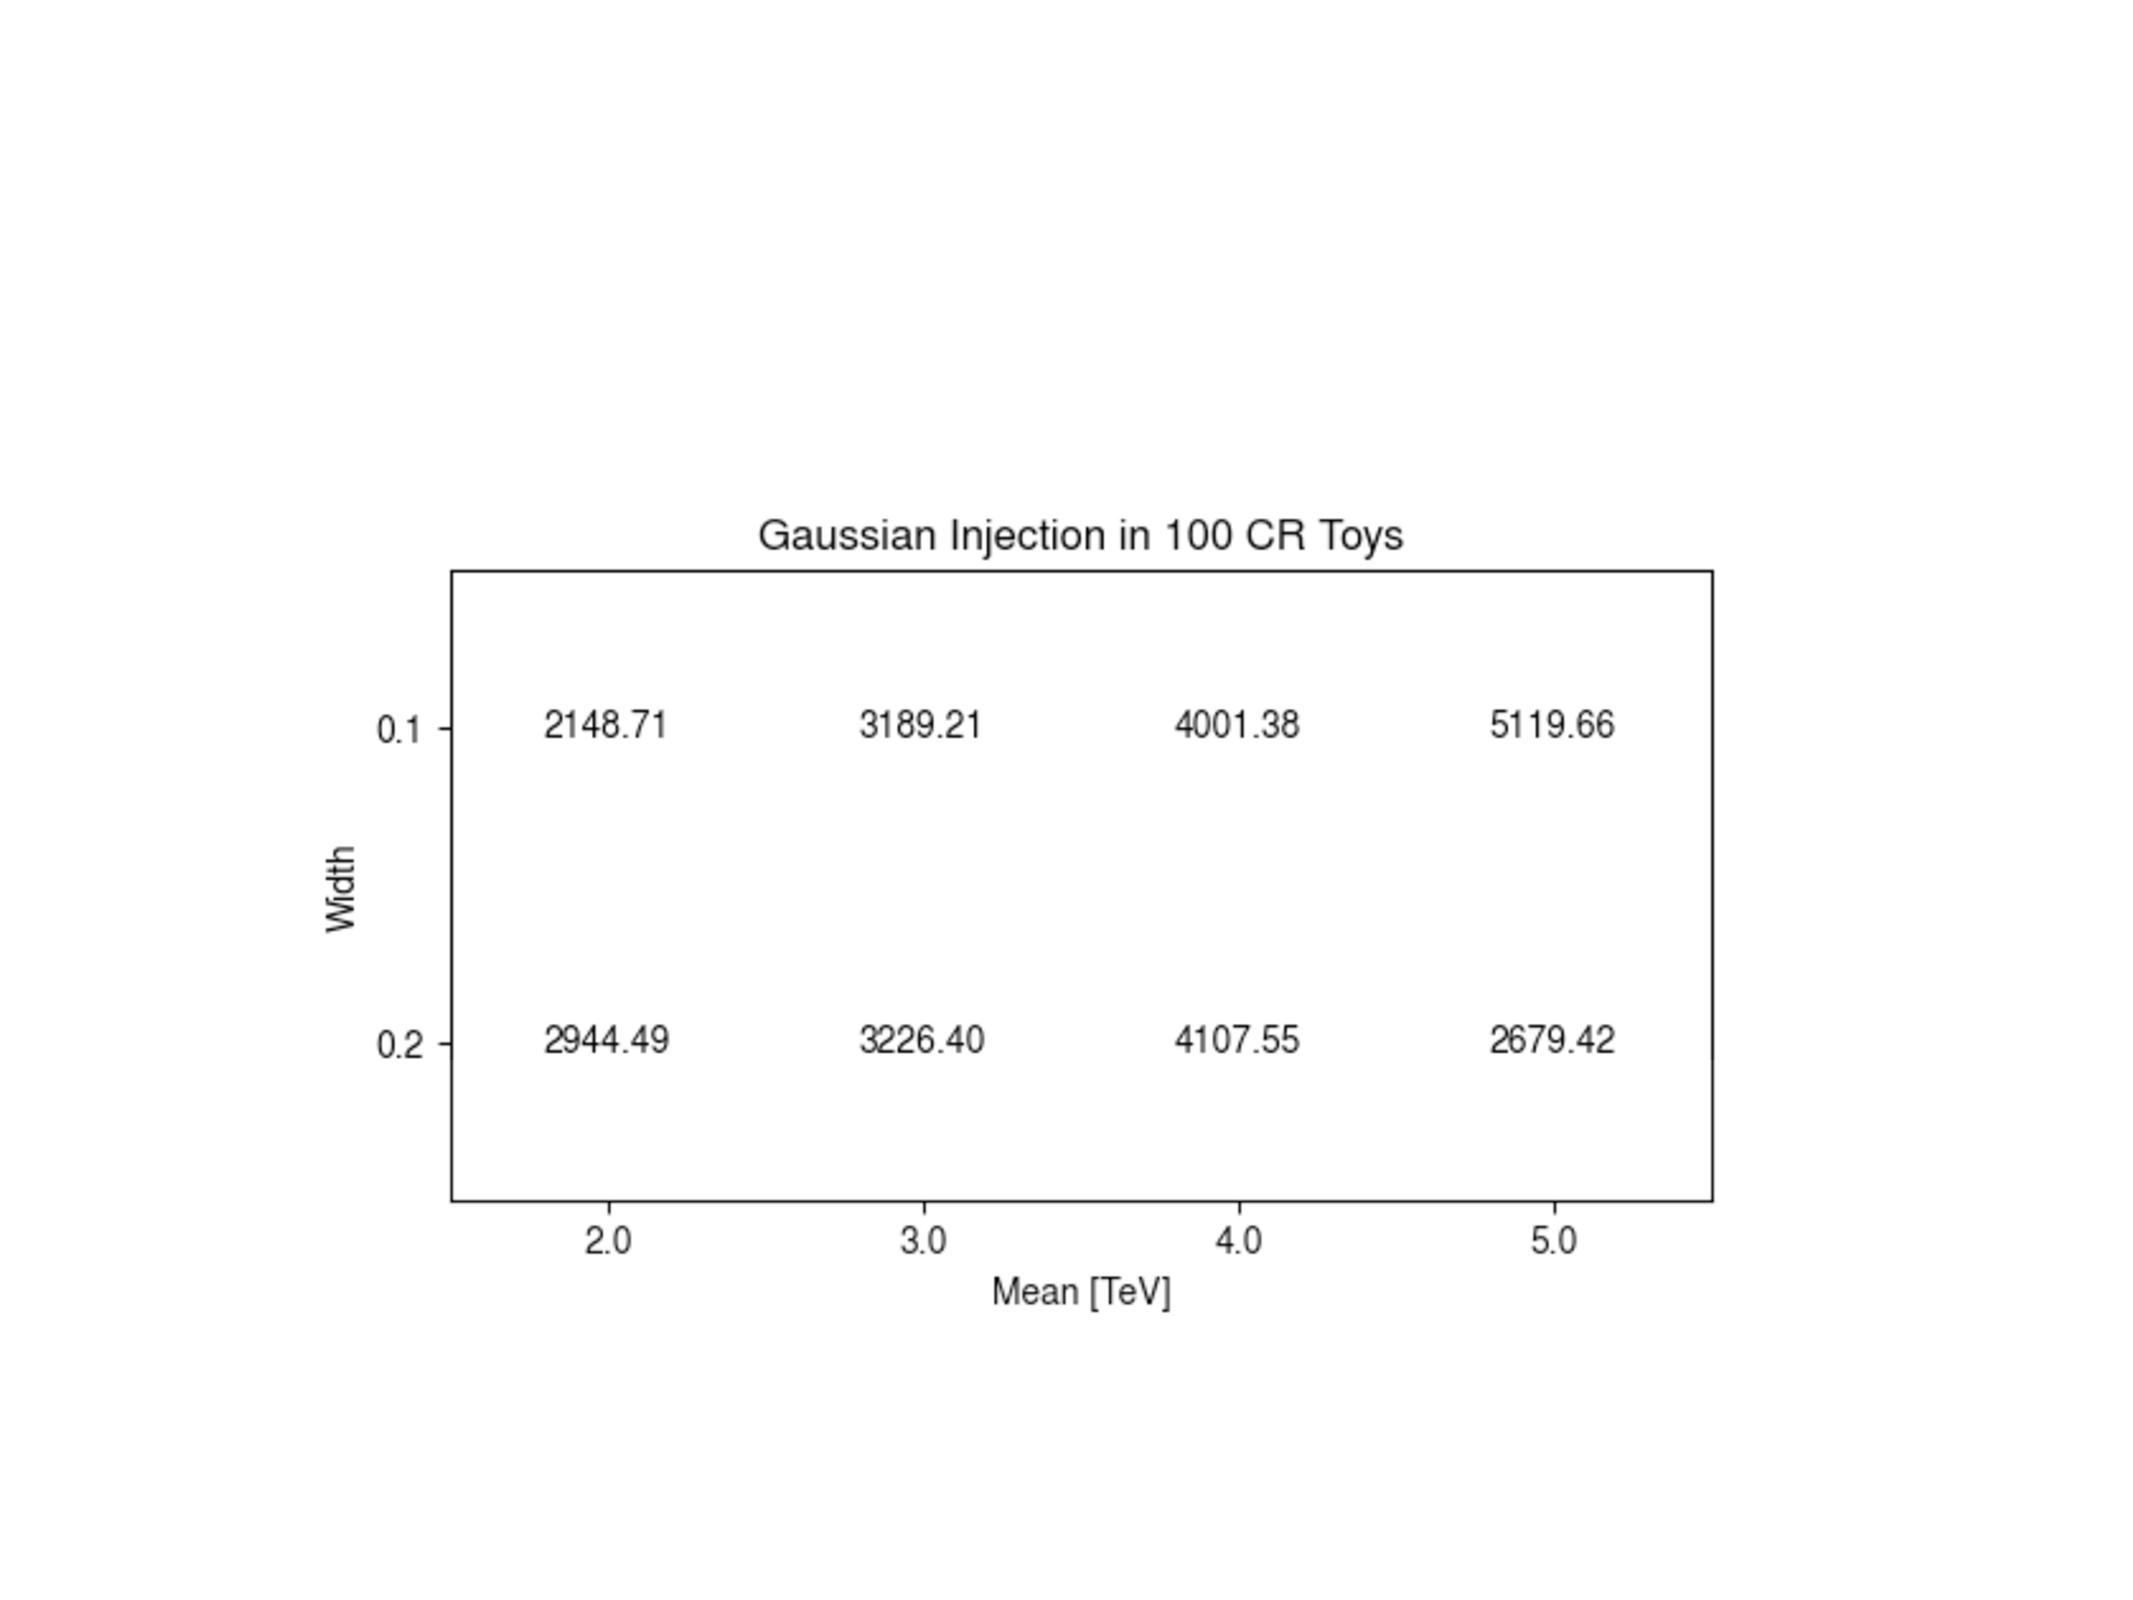
\includegraphics[width=0.65\textwidth]{figures/stats/siginj_bh_bumploc.pdf}
    \caption{Response of the BumpHunter framework to signal injection of $5\sigma$ significance to the model-dependent polynomial fit framework. The local significance (top) and bump location (bottom) are shown.
    \label{fig:siginj_bh}}
\end{figure}

\begin{figure}[!htbp]
\centering
   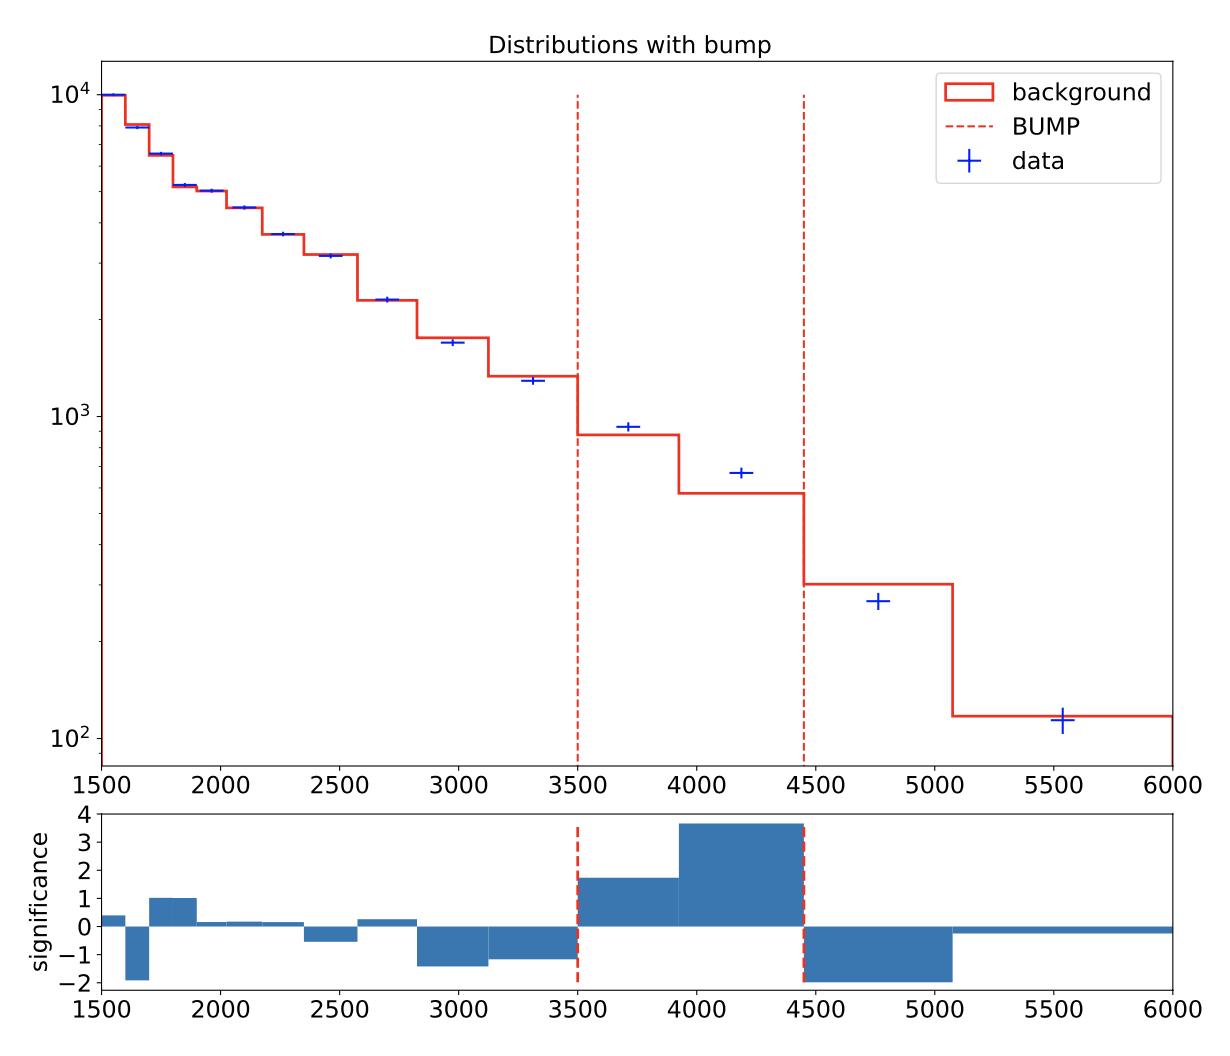
\includegraphics[width=0.5\textwidth]{figures/stats/bh_bump_example}
    \caption{Example BH response to gaussian signal injection at 4000 GeV with width of 10\%. 
    \label{fig:bh_bump_example}}
\end{figure}

%The BH significance can be slightly enhanced by repeating the polynomial fit after blinding the the most significant bump.
%This serves to ``flatten" the fit, allowing the bump to be more significant compared to the the background distribution. 
%This process is illustrated in Figure~\ref{fig:bh_masked}. 
%This strategy has the potential impact of enhancing non-signal deviations in the fit as well.
%Therefore, both BH results are considered together.

%\begin{figure}[!htbp]
%\centering
%   \includegraphics[width=0.95\textwidth]{figures/stats/bh_mask_before.pdf}
%   \includegraphics[width=0.95\textwidth]{figures/stats/bh_mask_after.pdf}
%    \caption{Improvement of the BH response after masking the region []redoing the polynomial background fit
%    \label{fig:siginj_bh}}
%\end{figure}

